\section{~Governing equations} \label{chapt:eq}
\newcounters

\vssub
\subsection{~Introduction} \label{sec:intro}
\vssub

Waves or spectral wave components in water with limited depth and non-zero
mean currents are generally described using several phase and amplitude
parameters. Phase parameters are the wavenumber vector {\bk}, the wavenumber
$k$, the direction $\theta$ and several frequencies. If effects of mean
currents on waves are to be considered, a distinction is made between the
relative or intrinsic (radian) frequency $\sigma$ $(= 2 \pi f_r)$, which is
observed in a frame of reference moving with the mean current, and the
absolute (radian) frequency $\omega$ $(= 2 \pi f_a)$, which is observed in a
fixed frame of reference.  The direction $\theta$ is by definition
perpendicular to the crest of the wave (or spectral component), and equals the
direction of {\bk}. Equations given here follow the geometrical optics approximation, 
which is exact in the limit when scales of variation of depths and currents are
 much larger than those of an individual wave\footnote{Even with a factor 5 change in wave height over half a wavelength, 
 the geometrical optics approximation can provide reasonable results as was shown over submarine canyons \citep{art:Mea07}}. 
 Diffraction, scattering and interference effects that are neglected by this approximation can be 
 added a posteriori as source terms in the wave action equation. Under this approximation of slowly varying 
 current and depth, the quasi-uniform
(linear) wave theory then can be applied locally, giving the following
dispersion relation and Doppler-type equation to interrelate the phase
parameters

%-----------------------------------%
% dispersion and Doppler equations  %
%-----------------------------------%
% eq:disp
% eq:doppler

\begin{equation}
\sigma ^2 = g k \tanh kd \: ,
\label{eq:disp}
\end{equation}
\begin{equation}
\omega = \sigma + {\bk} \cdot {\bf U} \: ,
\label{eq:doppler}
\end{equation}

\noindent 
where $d$ is the mean water depth and {\bf U} is the (depth- and time-
averaged over the scales of individual waves) current velocity. The assumption
of slowly varying depths and currents implies a large-scale bathymetry, for
which wave diffraction can generally be ignored. The usual definition of {\bk}
and $\omega$ from the phase function of a wave or wave component implies that
the number of wave crests is conserved \citep[see, e.g.,][]{bk:Phi77,bk:Mei83}

%-----------------------------%
% conservation of wave crests %
%-----------------------------%
% eq:wnconv

\begin{equation}
\frac{\partial {\bk}}{\partial t} + \nabla \omega = 0 \: .
\label{eq:wnconv}
\end{equation}

%\noindent

From Eqs.~(\ref{eq:disp}) through (\ref{eq:wnconv}) the rates of change of the
phase parameters can be calculated \citep[e.g.,][equations not reproduced
here]{rep:Chr82,bk:Mei83,tol:JPO90}.

%For monochromatic waves, the amplitude is described as the amplitude, the wave
%height, or the wave energy. 
For irregular wind waves, the (random) variance of
the sea surface is described using the surface elevation variance density spectrum $F$ . In the wave
modeling community this is usually called the  `energy spectrum'. This spectrum
$F$ is a function of all independent phase parameters, i.e.,
$F({\bk},\sigma,\omega)$, and furthermore varies in space and time at scales
larger than those of individual waves, e.g., $F({\bk},\sigma,\omega
;\bx,t)$. However, for waves shorter than 3 times the dominant wind sea frequency \citep{Leckler&al.2015}, 
the energy is very close to the linear dispersion relation so that
Eqs.~(\ref{eq:disp}) and (\ref{eq:doppler}) interrelate {\bk}, $\sigma$ and
$\omega$. Consequently only two independent phase parameters exist, and the
local and instantaneous spectrum becomes two-dimensional. The effect of non-linear contributions of 
bound waves can be added in \ws\ as post-processing, following the method of \cite{art:Jan09}.

Within \ws\ the
basic spectrum is the wavenumber-direction spectrum $F(k,\theta)$, which has
been selected because of its invariance characteristics with respect to
physics of wave growth and decay for variable water depths. The output of \ws,
however, consists of the more traditional frequency-direction spectrum
$F(f_r,\theta)$. The different spectra can be calculated from $F(k,\theta)$
using straightforward Jacobian transformations

%--------------------------------------------%
% Jacobian transformation and group velocity %
%--------------------------------------------%
% eq:jac_fr
% eq:jac_fa
% eq:cg

\begin{equation}
F(f_r,\theta) = \frac{\partial k}{\partial f_r} F(k,\theta) =
\frac{2\pi}{c_g} F(k,\theta) \: ,
\label{eq:jac_fr}
\end{equation}
\begin{equation}
F(f_a,\theta) = \frac{\partial k}{\partial f_a} F(k,\theta) =
\frac{2\pi}{c_g}
\left ( 1 + \frac{{\bk}\cdot{\bf U}}{k c_g}\right )^{-1}
F(k,\theta) \: ,
\label{eq:jac_fa}
\end{equation}
\begin{equation}
c_g = \frac{\partial \sigma}{\partial k} = n \frac{\sigma}{k}
\; , \;
n = \frac{1}{2} + \frac{kd}{\sinh 2kd} \; ,
\label{eq:cg}
\end{equation}

\noindent 
where $c_g$ is the group velocity.  From any of these spectra
one-dimensional spectra can be generated by integration over directions,
whereas integration over the entire spectrum by definition gives the total
variance $E$ (in the wave modeling community usually denoted as the wave
energy).

In cases without currents, the variance (energy) of a wave packet is a
conserved quantity. In cases with currents the energy or variance of a
spectral component is no longer conserved, due to the work done by current on
the mean momentum transfer of waves \citep{art:LHS61,art:LHS62}. In a general
sense, however, wave action $A \equiv E/\sigma$ is conserved
\citep[e.g.,][]{art:Whi65,art:BG68}. This makes the wave action density
spectrum $N(k,\theta) \equiv F(k,\theta)/\sigma$ the spectrum of choice within
the model. Wave propagation then is described by

%--------------------------------------%
% Most general action balance equation %
%--------------------------------------%
% eq:balance0

\begin{equation}
\frac{D N}{D t} = \frac{S}{\sigma} \: ,
\label{eq:balance0}
\end{equation}

\noindent 
where $D/Dt$ represents the total derivative (moving with a wave component)
and $S$ represents the net effect of sources and sinks for the spectrum
$F$. Because the left side of Eq.~(\ref{eq:balance0}) generally considers
linear propagation without scattering, effects of nonlinear wave propagation
(i.e., wave-wave interactions) and partial wave reflections arise in
$S$. Propagation and source terms will be discussed separately in the
following sections.

\vssub
\subsection{~Propagation}
\vssub

In a numerical model, an Eulerian form of the balance equation
(\ref{eq:balance0}) is needed. This balance equation can either be written in
the form of a transport equation (with velocities outside the derivatives), or
in a conservation form (with velocities inside the derivatives). The former
form is valid for the vector wavenumber spectrum $N(\bk;\bx,t)$ only, whereas
valid equations of the latter form can be derived for arbitrary spectral
formulations, as long as the corresponding Jacobian transformation as
described above is well behaved \citep[e.g.,][]{tol:GAOS98b}. Furthermore, the
conservation equation conserves total wave energy/action, unlike the transport
equation. This is an important feature of an equation when applied in a
numerical model. The balance equation for the spectrum $N(k,\theta;\bx,t)$ as
used in \ws\ is given as (for convenience of notation, the spectrum is
henceforth denoted simply as $N$):

%----------------------------------%
% Plain-grid propagation equations %
%----------------------------------%
% eq:bal_plane
% eq:x_dot
% eq:k_dot
% eq:theta_dot

\begin{equation}
\frac{\partial N}{\partial t} + \nabla_x \cdot {\bf\dot{x}}N +
\frac{\partial}{\partial k} \dot{k}N +
\frac{\partial}{\partial \theta} \dot{\theta}N =
\frac{S}{\sigma} \: , \label{eq:bal_plane}
\end{equation}
\begin{equation}
{\bf \dot{x}} = {\bf c}_g + {\bf U} \: , \label{eq:x_dot}
\end{equation}
\begin{equation}
\dot{k} = - \frac{\partial \sigma}{\partial d}
\frac{\partial d}{\partial s} - {\bk} \cdot
\frac{\partial {\bf U}}{\partial s} \: , \label{eq:k_dot}
\end{equation}
\begin{equation}
\dot{\theta} = - \frac{1}{k} \left [
\frac{\partial \sigma}{\partial d} \frac{\partial d}{\partial m}
+ {\bk} \cdot \frac{\partial {\bf U}}{\partial m}
\right ] \: , \label{eq:theta_dot}
\end{equation}

\noindent
where ${\bf c}_g = (c_g \sin \theta, c_g \cos \theta$, $s$ is a coordinate in the
direction $\theta$ and $m$ is a coordinate perpendicular to $s$.
Equation~(\ref{eq:bal_plane}) is valid for Cartesian coordinates. For large-scale
applications, this equation is usually transferred to spherical coordinates,
defined by longitude $\lambda$ and latitude $\phi$, but maintaining the
definition of the local variance \citep[i.e., per unit surface, as
in][]{art:WAM88}

%---------------------------------%
% Spherical propagation equations %
%---------------------------------%
% eq:bal_sphere
% eq:phi_dot
% eq:lambda_dot
% eq:theta_g_dot

\begin{equation}
\frac{\partial N}{\partial t} +
\frac{1}{\cos \phi} \frac{\partial}{\partial \phi} \dot{\phi}
    N \cos \theta +
\frac{\partial}{\partial \lambda} \dot{\lambda}N +
\frac{\partial}{\partial k} \dot{k} N +
\frac{\partial}{\partial \theta} \dot{\theta}_g N
= \frac{S}{\sigma} \: ,\label{eq:bal_sphere}
\end{equation}
\begin{equation}
\dot{\phi} = \frac{c_g \cos \theta + U_\phi}{R}
\: , \label{eq:phi_dot}
\end{equation}
\begin{equation}
\dot{\lambda} =  \frac{c_g \sin \theta + U_\lambda}{R \cos \phi}
\: , \label{eq:lambda_dot}
\end{equation}
\begin{equation}
\dot{\theta}_g = \dot{\theta} -
\frac{c_g \tan \phi \cos \theta}{R}
\: , \label{eq:theta_g_dot}
\end{equation}

\noindent
where $R$ is the radius of the earth and $U_\phi$ and $U_\lambda$ are current
components. Equation~(\ref{eq:theta_g_dot}) includes a correction term for
propagation along great circles, using a Cartesian definition of $\theta$
where $\theta = 0$ corresponds to waves traveling from west to east. \ws\ can
be run using either Cartesian or Spherical coordinates. Note that unresolved obstacles
such as islands can be included in the equations. In \ws\ this is done at the
level of the numerical scheme, as is discussed in section~\ref{sub:num_obst}. Also, depth variations 
at the scale of the wavelength can be introduced by a scattering source term described in 
 section~\ref{sec:BS1}. 
 
 Finally, both Cartesian  and spherical coordinates can be discretized in many ways, using quadrangles (rectangular, curvilinear or SMC grids) and triangles. 
That aspect is treated in chapter~\ref{chapt:num}.

\vssub
\subsection{~Non-ice source term integration} \label{sub:source}
\vssub

The source terms not involving ice are accounted for by solving

%---------------------%
% Step : Source terms %
%---------------------%
% eq:step_source

\begin{equation}
\frac{\p N}{\p t} = \cS_{no~ice} \: . \label{eq:step_source}
\end{equation}

\noindent 
As in \wam, a semi-implicit integration scheme is used. In this scheme the
discrete change of action density $\Delta N$ becomes \citep{art:WAM88}

% eq:implicit_st

\begin{equation}
\Delta N(k,\theta) = \frac{\cS(k,\theta)}{1- \epsilon D(k,\theta)\Delta t}
\: , \label{eq:implicit_st} \end{equation}

\noindent 
where $D$ represents the diagonal terms of the derivative of $\cS$ with
respect to $N$ \citep[Eqs. 4.1 through 4.10]{art:WAM88}, and where $\epsilon$
defines the offset of the scheme. Originally, $\epsilon = 0.5$ was implemented
to obtain a second-order accurate scheme. Presently, $\epsilon = 1$ is used because it is more appropriate for the large time steps in the equilibrium range of
the spectrum \citep{pro:HA98,art:HA01} and it results in much smoother
integration of the spectrum. The change of $\epsilon$ has little impact on
mean wave parameters, but makes the dynamical time stepping as described below
more economical.

The semi-implicit scheme is applied in the framework of a dynamic
time-stepping scheme \citep{tol:JPO92}. In this scheme, integration over the
global time step $\Delta t_g$ can be performed in several dynamic time steps
$\Delta t_d$, depending on the net source term $\cS$, a maximum change of
action density $\Delta N_m$ and the remaining time in the interval $\Delta
t_g$. For the $n^{\rm th}$ dynamic time step in the integration over the
interval $\Delta t_g$, $\Delta t_d^n$ is calculated in three steps as

% ------ Dynamic s.t. int. scheme ------- %
% eq:st_d_1
% eq:st_d_2a
% eq:st_d_2b
% eq:st_d_3

\begin{equation}
\Delta t_d^n = 
\min_{f<f_{hf}} \left [ \frac{\Delta N_m}{|\cS|}
\left ( 1 + \epsilon D \frac{\Delta N_m}{|\cS|} \right ) ^{-1}
\right ] \: , \label{eq:st_d_1}
\end{equation} \begin{equation}
\Delta t_d^n = \max \: \left [ \: \Delta t_d^n \: , \: 
\Delta t_{d,\min} \right ] \: , \label{eq:st_d_2a}
\end{equation} \begin{equation}
\Delta t_d^n = \min \: \left [ \: \Delta t_d^n \: , \: 
\Delta t_g - \sum_{i=1}^{n-1} \Delta t_d^i
 \: \right ] \: , \label{eq:st_d_2b}
\end{equation}

\noindent
where $\Delta t_{\min}$ is a user-defined minimum time step, which is added to
avoid excessively small time steps. The corresponding new spectrum $N^n$
becomes

\begin{equation}
N^n = \max\: \left [ \: 0 \: , \: N^{n-1} + 
\left ( \frac{\cS \Delta t_d}{1 - \epsilon D \Delta t_d} \right )
\: \right ] \: . \label{eq:st_d_3}
\end{equation}


The maximum change of action density $\Delta N_m$ is determined from a
parametric change of action density $\Delta N_p$ and a filtered relative
change $\Delta N_r$

% eq:st_d_4
% eq:st_d_5
% eq:st_d_6
% eq:st_d_7

\begin{equation}
\Delta N_m (k,\theta) = \min \: \left [ \:
\Delta N_p (k,\theta) \: , \: \Delta N_r (k,\theta) 
\: \right ] \: , \label{eq:st_d_4}
\end{equation} \begin{equation}
\Delta N_p (k,\theta) = X_p \: \frac{\alpha}{\pi} \:
\frac{(2\pi)^4}{g^2} \: \frac{1}{\sigma k^3}
\: , \label{eq:st_d_5}
\end{equation} \begin{equation}
\Delta N_r (k,\theta) = X_r \; \max \: \left [ \: 
N(k,\theta) \: , \: N_f \: \right ] \: , \label{eq:st_d_6}
\end{equation} \begin{equation}
N_f = \max \: \left [ \: \Delta N_p (k_{\max},\theta) \: , 
\: X_f \: \max_{\forall k,\theta} \left \{ N(k,\theta) \right \}
\: \right ] \: , \label{eq:st_d_7} \end{equation}

\noindent 
where $X_p$, $X_r$ and $X_f$ are user-defined constants (see
Table~\ref{tab:st_d_p}), $\alpha$ is a {\sc pm} spectrum energy level (set to $\alpha =
0.62\times 10^{-4}$) and $k_{\max}$ is the maximum discrete wavenumber. The
parametric spectral shape in (\ref{eq:st_d_5}) corresponds in deep water to
the well-known high-frequency shape of the one-dimensional frequency spectrum
$F(f) \propto f^{-5}$. The link between the filter level and the maximum
parametric change in (\ref{eq:st_d_7}) is used to assure that the dynamic time
step remains reasonably large in cases with extremely small wave energies. A
final safeguard for stability of integration is provided by limiting the
discrete change of action density to the maximum parametric change
(\ref{eq:st_d_5}) in conditions where Eq.~(\ref{eq:st_d_2a}) dictates $\Delta
t_d^n$. In this case Eq.~(\ref{eq:st_d_2a}) becomes a limiter as in the WAM
model. Impacts of limiters are discussed in detail in for instance
\cite{art:HJ99,art:HJ01}, \cite{art:HA01} and \cite{tol:GAOS02}.

% tab:st_d_p

\begin{table} 
\begin{center} \begin{tabular}{|l|c|c|c|c|} \hline \hline
                 & $X_p$     & $X_r$             & $X_f$ &
$\Delta t_{d,\min}$      \\ \hline
\wam\ equivalent & $\frac{\pi}{24}10^{-3}\Delta t$
 & $\infty (\geq 1)$ & --    & $\Delta t_g$  \\ 
 suggested       & 0.1-0.2  & 0.1-0.2 & 0.05 & $\approx 0.1 \Delta t_g$ \\  
default setting  &  0.15    &   0.10  & 0.05 & -- \\ \hline \hline
\end{tabular} \end{center}
\caption{User-defined parameters in the source term integration
 scheme}
\label{tab:st_d_p} \botline \end{table}

The dynamic time step is calculated for each grid point separately, adding
additional computational effort only for grid points in which the spectrum is
subject to rapid change. The source terms are re-calculated for every dynamic
time step.

It is possible to compile \ws\ without using a linear growth term. In such a
case, waves can only grow if some energy is present in the spectrum. In
small-scale applications with persistent low wind speeds, wave energy might
disappear completely from part of the model. To assure that wave growth can
occur when the wind increases, a so-called seeding option is available in \ws\
(selected during compilation). If the seeding option is selected, the energy
level at the seeding frequency $\sigma_{\rm seed} = \min(\sigma_{\max}, 2\pi
f_{hf})$ is required to at least contain a minimum action density

% ------ Spectral seeding ------- %
% eq:seed

\begin{eqnarray}
N_{\min}(k_{seed},\theta) & = & 
        6.25 \times 10^{-4} \frac{1}{k_{\rm seed}^3 \: \sigma_{\rm seed}}
        \max \left [ \: 0. \: , \: \cos^2 ( \theta - \theta_w ) \right ]
                             \nonumber \\ & & \hspace{5mm}
        \min \left [ \: 1 \: , \: \max \left ( \: 0 \: , \: 
        \frac{|u_{10}|}{X_{\rm seed} g \sigma_{\rm seed}^{-1}}-1 
\: \right ) \: \right ] \: , \label{eq:seed} \end{eqnarray}

\noindent
where $g \sigma_{\rm seed}^{-1}$ approximates the equilibrium wind speed for
the highest discrete spectral frequency. This minimum action distribution is
aligned with the wind direction, goes to zero for low wind speeds, and is
proportional to the integration limiter (\ref{eq:st_d_5}) for large wind
speeds. $X_{\rm seed} \geq 1$ is a user-defined parameter to shift seeding to
higher frequencies. Seeding starts if the wind speed reaches $X_{\rm seed}$
times the equilibrium wind speed for the highest discrete frequency, and
reaches its full strength for twice as high wind speeds. The default model
settings include the seeding algorithm, with $X_{\rm seed} = 1$.

In model version 3.11, surf-zone physics parameterizations have been
introduced. Such physics, particularly depth-induced breaking, operate on much
smaller time scales than deep water and limited-depth physics outside the surf
zone. To assure reasonable behavior for larger time steps, an additional
optional limiter has been adopted from the SWAN model, which can be used instead of 
modeling surf-breaking explicitly.  This limiter is similar to the Miche
style maximum wave height in the depth-limited wave breaking source term of
Eq.~(\ref{eq:BJ78_Miche}). In this limiter, the maximum wave energy $E_m$ is
computed as

% ------ Surf zone limiter ------ %
% eq:MLIM

\begin{equation}
E_m = \frac{1}{16} [ \gamma_{lim}  \tanh ( \bar{k} d ) / \bar{k} ] ^2
\:\:\: , \label{eq:MLIM} 
\end{equation}

\noindent
where $\gamma_{lim}$ is a factor comparable to $\gamma_M$ in
Eq.~(\ref{eq:BJ78_Miche}), with the caveat that $\gamma_M$ is representative
for an individual wave, whereas $\gamma_{lim}$ is representative for the
significant wave height. For monochromatic waves, the original expression by
\cite{art:Miche44} would correspond to $\gamma_{lim} = 0.94$ and replacing
$H_s$ by the height $H$ of the waves. Here this idea is applied to random
waves.  In shallow water, this limits $H_s$ to be less than $\gamma_{lim} d$.
If the total spectral energy $E$ is larger than the maximum energy $E_m$, the
limiter is applied by simply rescaling the spectrum by the factor $E/E_m$,
loosely following the argumentation from \cite{art:EB96} and used
in \para\ref{sec:DB1}.  

This limiter can be switched on or off in the
compilation of the model, and $\gamma_{lim}$ can be adjusted by the user. The
default is set to $\gamma_{lim} = 1.6$ because $H_{rms}$ values close to $d$
have indeed been recorded and thus taking a ratio $H_s/H_{rms}$ of 1.4, using
1.6 allows this large steepness to be exceeded by some margin.  Note that this
limiter should be used as a `safety valve' only, and hence that it should be
less strict than the breaking criterion in the surf-breaking or whitecapping
source terms, if these source terms are modeled explicitly.

Also, this limiter does not guarantee that all parts of the spectrum are
realistic. Indeed, the use of a mean wavenumber, as in the Komen et
al. dissipation, makes it possible to have unrealistically steep short waves
in the presence of swell. A future extension of this limiter could be to limit
the steepness with a partial spectral integration in frequencies, to make sure
that waves of all scales are indeed not too steep.

\vssub
\subsection{~Ice source terms integration} \label{sub:icesource}
\vssub

Because the attenuation and scattering in the ice can be very strong (although they are linear), it is convenient 
to perform a separate integration of the ice terms $S_{\mathrm{ice}}=S_{\mathrm{id}}+S_{\mathrm{is}}$. This combines 
a dissipation term 
\begin{equation}
S_{\mathrm{id}}/\sigma  = \beta_{\mathrm{id}} N ,
\end{equation}
 and a scattering term 
which is of the form 
\begin{equation}
 \frac{S_{\mathrm{is}}(k,\theta)}{\sigma} =  \int_0^{2\pi}\beta_{\mathrm{is}} [N(k,\theta')-N(k,\theta)] d\theta'  ,
 \end{equation}
 in which the scattering coefficient $\beta_{\mathrm{is}}$ is a priori a function of the difference in direction between 
 incident $\theta'$ and scattered $\theta$ directions, as well as the shape of ice floes. In general 
  the directional spectrum $N(k,.)$ is a vector with {\F NTH} (number of directions) components, 
and the source term is a vector of the same size  given by the matrix product $S/\sigma = M N(k,.)$ where  
$M$ is a positive symmetric square {\F NTH} by {\F NTH} matrix with components given from the $\beta_{\mathrm{id}}$ values.
The matrix $M$ is easily diagonalized as 
\begin{equation}
 M  =  V D V^T  ,
 \end{equation}
 where $D$ is a diagonal matrix containing all eigenvalues and $V$ is the array of eigenvectors, 
 and $V^T$ is its transpose. As a result the split wave action equation for ice source terms 
 \begin{equation}
\frac{\p}{\p t} \frac{N}{c_g}   = \frac{S_{\mathrm{id}}}{\sigma c_g} ,
 \end{equation}
 can be rewritten for the action $N_i$ of each eigenvector $V_i$ with eigenvalue $\lambda_i$ as 
  \begin{equation}
\frac{\p}{\p t} \frac{N_i}{c_g}   = \frac{\beta_{\mathrm{id}} + \lambda_i}{\sigma c_g} N_i ,
 \end{equation}
 which has the following exact solution 
   \begin{equation}
 {N_i}(t+\Delta t_g)   = N_i(t) \exp \left[ (\beta_{\mathrm{id}} + \lambda_i) +\Delta t_g\right].
 \end{equation}
 
 In all cases the eigenvector corresponding to an isotropic spectrum has an eigenvalue $\lambda=\beta_{\mathrm{id}}$. 
 In the case of an isotropic back-scatter, the other eigenvalues are all equal to $(\beta_{\mathrm{id}} + \beta_{\mathrm{is}})$. 
 This decomposition over the two eigenspaces simplifies the solution to 
%---------------------%
% Step : Source terms %
%---------------------%
% eq:exact_st_ice
\begin{equation}
 N(t+\Delta t_g) = \exp(\beta_{\mathrm{id}} \Delta t_g) \overline{N}(t)  + \exp \left[\left(\beta_{\mathrm{id}} + \beta_{\mathrm{is}}\right) \Delta t_g\right] \left[N(t)-\overline{N}(t)\right]
, \label{eq:exact_st_ice} \end{equation}
where $\overline{N}$ is the average over all directions. As a result, for a spatially homogeneous field, 
the spectrum exponentially tends to isotropy over a time scale $1/(\beta_{\mathrm{id}})$.

\vsssub
\subsubsection{~$S_{nl}$: Discrete Interaction Approximation (\dia)} \label{sec:NL1}
\vsssub

\opthead{NL1}{\wam\ model}{H. L. Tolman}

\noindent
Nonlinear wave-wave interactions can be modeled using the discrete interaction
approximation \citep[\dia,][]{art:Hea85b}. This parameterization was
originally developed for the spectrum $F(f_r ,\theta)$. To assure the
conservative nature of $S_{nl}$ for this spectrum (which can be considered as
the "final product" of the model), this source term is calculated for
$F(f_r,\theta)$ instead of $N(k,\theta)$, using the conversion
(\ref{eq:jac_fr}).

Resonant nonlinear interactions occur between four wave components
(quadruplets) with wavenumber vector $\bk_1$ through $\bk_4$. In the \dia, it
is assumed that $\bk_1 = \bk_2$. Resonance conditions then require that
%--------------------------%
% Resonance conditions DIA %
%--------------------------%
% eq:resonance
\begin{equation} \left .
\begin{array}{ccc}
  \bk_1 + \bk_2 & = & \bk_3 + \bk_4          \\
  \sigma_2  & = & \sigma_1                   \\
  \sigma_3  & = & (1+\lambda_{nl})\sigma_1   \\
  \sigma_4  & = & (1-\lambda_{nl})\sigma_1
\end{array} \:\:\: \right \rbrace \:\:\: , \label{eq:resonance}
\end{equation}
where $\lambda_{nl}$ is a constant. For these quadruplets, the contribution
$\delta S_{nl}$ to the interaction for each discrete $(f_r,\theta)$
combination of the spectrum corresponding to $\bk_1$ is calculated as
%----------------------------%
% Nonlinear interactions DIA %
%----------------------------%
% eq:snl_dia
\begin{eqnarray}
\left ( \begin{array}{c}
  \delta S_{nl,1} \\ \delta S_{nl,3} \\ \delta S_{nl,4}
\end{array} \right ) & = & D
\left ( \begin{array}{r} -2 \\ 1 \\ 1 \end{array} \right )
C g^{-4} f_{r,1}^{11} \times \nonumber \\
& & \left [ F_1^2
\left ( \frac{F_3}{(1+\lambda_{nl})^4} +
        \frac{F_4}{(1-\lambda_{nl})^4} \right ) -
\frac{2 F_1 F_3 F_4}{(1-\lambda_{nl}^2)^4}
\right ] \: , \label{eq:snl_dia}
\end{eqnarray}
where $F_1 = F(f_{r,1} ,\theta_1 )$ etc. and $\delta S_{nl,1} = \delta
S_{nl}(f_{r,1} ,\theta_1 )$ etc., $C$ is a proportionality constant. The
nonlinear interactions are calculated by considering a limited number of
combinations $(\lambda_{nl},C)$. In practice, only one combination is
used. Default values for different source term packages are presented in
Table~\ref{tab:snl_par}.


% tab:snl_par

\begin{table} \begin{center}
 \begin{tabular}{|l|c|c|} \hline
                    & $\lambda_{nl}$ &     $C$      \\ \hline
ST6                 &      0.25      & $3.00 \; 10^7$  \\ \hline
\wam-3              &      0.25      & $2.78 \; 10^7$  \\ \hline
ST4 (Ardhuin et al.)&      0.25      & $2.50 \; 10^7$  \\ \hline
Tolman and Chalikov &      0.25      & $1.00 \; 10^7$  \\ \hline
\end{tabular} \end{center}
\caption{Default constants in \dia\ for input-dissipation packages.}
\label{tab:snl_par} \botline \end{table}

This source term is developed for deep water, using the appropriate dispersion
relation in the resonance conditions. For shallow water the expression is
scaled by the factor $D$ (still using the deep-water dispersion relation,
however)

%------------------%
% Depth factor DIA %
%------------------%
% eq:snl_shal

\begin{equation}
D = 1 + \frac{c_1}{\bar{k}d} \left [ 1 - c_2 \bar{k} d
\right ] e^{-c_3 \bar{k} d} \: . \label{eq:snl_shal}
\end{equation}

\noindent
Recommended (default) values for the constants are $c_1=5.5$, $c_2=5/6$ and
$c_3=1.25$ \citep{art:Hea85a}. The overbar notation denotes straightforward
averaging over the spectrum. For an arbitrary parameter $z$ the spectral average
is given as

%--------------------------%
% Definition spectral mean %
%--------------------------%
% eq:zbar
% eq:etot

\begin{equation}
\bar{z} = E^{-1} \int_{0}^{2\pi} \int_{0}^{\infty}
z F(f_r,\theta) \; d f_r \; d\theta \: , \label{eq:zbar}
\end{equation}
\begin{equation}
E = \int_{0}^{2\pi} \int_{0}^{\infty}
F(f_r,\theta) \; d f_r \; d\theta \: . \label{eq:etot}
\end{equation}

\noindent
For numerical reasons, however, the mean relative depth is estimated as

%------------%
% kd for DIA %
%------------%
% eq:kd_num
% eq:k_hat

\begin{equation}
\bar{k} d = 0.75 \hat{k} d \: , \label{eq:kd_num}
\end{equation}

\noindent
where $\hat{k}$ is defined as

\begin{equation}
\hat{k} = \left ( \overline{1/\sqrt{}k} \right )^{-2} \: .
\label{eq:k_hat}
\end{equation}

\noindent
The shallow water correction of Eq.~(\ref{eq:snl_shal}) is valid for
intermediate depths only. For this reason the mean relative depth
$\bar{k}d$ is not allowed to become smaller than 0.5 (as in \wam). All
above constants can be reset by the user in the input files of the
model (see \para\ref{sub:ww3grid}).


\vsssub
\subsubsection{~$S_{nl}$: Full Boltzmann Integral (WRT)} \label{sec:NL2}
\vsssub

\opthead{NL2}{Exact-NL model}{G. Ph. van Vledder}

\noindent
The second method for calculating the nonlinear interactions in \ws\ is the
so-called Webb-Resio-Tracy method (\xnl), which is based on the original work
on the six-dimensional Boltzmann integral formulation of
\cite{art:Has62,art:Has63a,art:Has63b}, and additional considerations by
\cite{art:Web78}, \cite{rep:TR82} and \cite{art:RP91}.

The Boltzmann integral describes the rate of change of action density of a
particular wavenumber due to resonant interactions between pairs of four
wavenumbers. To interact, these wavenumbers must satisfy the following
resonance conditions

%--------------------------%
% Resonance conditions WRT %
%--------------------------%
% eq:resonance_2

\begin{equation} \left .
\begin{array}{ccc}
  \bk_1 + \bk_2 & = & \bk_3 + \bk_4          \\
  \sigma_1 + \sigma_2  & = & \sigma_3 + \sigma_4
\end{array} \:\:\: \right \rbrace \:\:\: , \label{eq:resonance_2}
\end{equation}

\noindent
which is a more general version of the resonance conditions
(\ref{eq:resonance}). The rate of change of action density $N_1 $ at
wavenumber $\bk_1$ due to all quadruplet interactions involving
$\bk_1$ is given by

\begin{eqnarray}
\frac{{\p N_1 }}{{\p t}} & = & \int\!\!\int\!\!\int G\left( \bk_1
,\bk_2 ,\bk_3 ,\bk_4 \right ) \: \delta \left( \bk_1  + \bk_2  - \bk_3
- \bk_4 \right)
\: \delta \left( {\sigma _1  + \sigma _2  - \sigma _3  - \sigma _4 }
\right) \nonumber \\  & &
\hspace{7mm}\times \:\:\: \left[ {N_1 N_3 \left( {N_4  - N_2 } \right)
+ N_2 N_4 \left(
{N_3  - N_1 } \right)} \right] \: d\bk_2 \: d\bk_3 \: d\bk_4 \:\:\: ,
\label{eq:HKE}
\end{eqnarray}

\noindent
where the action density $N$ is defined in terms of the wavenumber
vector $\bk$, $N = N(\bk)$. The term $G$ is a complicated coupling
coefficients for which expressions have been given by \cite{art:HH80}.
In the \xnl\ method a number of transformations are
made to remove the delta functions. A key element in the \xnl\ method
is to consider the integration space for each ($\bk_1 ,\bk_3 $)
combination \citep[see][]{art:RP91}

\begin{equation}
{{\partial N_1 } \over {\partial t}} = 2\int T\left( {\bk_1 ,\bk_3 }
\right) \: d\bk_3  \:\:\: ,
\end{equation}

\noindent
in which the function $T$ is given by

\begin{eqnarray}
T \left( \bk_1 ,\bk_3 \right) & = & \int\!\!\int
G\left( \bk_1 ,\bk_2, \bk_3 ,\bk_4 \right) \: \delta \left( \bk_1  +
\bk_2  - \bk_3  - \bk_4 \right) \nonumber \\
& \times & \delta \left( {\sigma _1  + \sigma _2  - \sigma _3  -
\sigma _4 }
\right) \: \theta \left ( \bk_1 , \bk_3 , \bk_4 \right )
\nonumber \\
& \times & \left [ N_1 N_3 \left ( N_4 - N_2 \right ) + N_2 N_4 \left
(
N_3  - N_1 \right ) \right ] \: d\bk_2 \: d\bk_4 \:\:\: ,
\label{eq:WRT_T}
\end{eqnarray}

\noindent
in which

\begin{equation}
\theta \left( {\bk_1 ,\bk_3 ,\bk_4 } \right) = \left\{ {\begin{array}{*{20}c}
   1 & {\rm{when}} & {\left| {\bk_1  - \bk_3 } \right| \leq \left| {\bk_1  - \bk_4 } \right|}  \\
   0 & {\rm{when}} & {\left| {\bk_1  - \bk_3 } \right| > \left| {\bk_1  - \bk_4 } \right|}  \\
 \end{array} } \right.
\end{equation}

The delta functions in Eq. (\ref{eq:WRT_T}) determine a region in wavenumber
space along which the integration should be carried out.  The function
$\theta$ determines a section of the integral which is not defined due to the
assumption that $\bk_1$ is closer to $\bk_3$ than $\bk_2$. The crux of the
Webb method consists of using a local coordinate system along a so-named
locus, that is, the path in $\bk$ space given by the resonance conditions for
a given combination of $\bk_1$ and $\bk_3$. To that end the $(k_{x},k_{y})$
coordinate system is replaced by a $(s,n)$ coordinate system, where $s$ ($n$)
is the tangential (normal) direction along the locus. After some
transformations, the transfer integral can then be written as a closed line
integral along the closed locus

\begin{eqnarray}
T \left( \bk_1 ,\bk_3 \right) & = & \oint G \:
\left | \frac{\p W(s,n)}{\p n}\right | ^{-1}
\: \theta ( \bk_1 , \bk_3 , \bk_4 ) \nonumber \\
& \times & \left [ N_1 N_3 \left ( N_4 - N_2 \right ) + N_2 N_4 \left
(
N_3  - N_1 \right ) \right ] \: d s  \:\:\: , \label{eq:WRT_T2}
\end{eqnarray}

\noindent
in which $G$ is the coupling coefficient and $\left| {\partial W/\partial n}
\right|$ is the gradient term of a function representing the resonance
conditions \citep[see][]{pro:vVl00}. Numerically, the Boltzmann integral is
computed as the finite sum of many line integrals $T$ for all discrete
combinations of $\bk_1$ and $\bk_3$. The line integral (\ref{eq:WRT_T2}) is
solved by dividing the locus in typically 30 pieces, such that the discretized
version is given as:

\begin{equation}
T\left( {\bk_1 ,\bk_3 } \right) \approx \sum_{i=1}^{n_s } G(s_i)
W(s_i) P(s_i) \: \Delta s_i \:\:\: ,
\end{equation}

\noindent
in which $P(s_i)$ is the product term for a given point on the locus,
$n_s$ is the number of segments, and $s_i$ is the discrete coordinate
along the locus. Finally, the rate of change for a given wavenumber
$\bk_1 $ is given by

\begin{equation}
\frac{\p N(\bk_1)}{\p t} \approx \sum_{i_{k3}  = 1}^{n_k }
{\sum_{i_{\theta 3}  = 1}^{n_\theta  } k_3 T(\bk_1,\bk_3) \: \Delta
k_{i_{k3}} \: \Delta \theta_{i_{\theta 3} } }, \label{eq:WRT_numT}
\end{equation}

\noindent
where $n_k$ and $n_\theta$ are the discrete number of wavenumbers and
directions in the computational grid, respectively. Note that although the
spectrum is defined in terms of the vector wavenumber $\bk$, the computational
grid in a wave model is more conveniently defined in terms of the absolute
wavenumber and wave direction ($k,\theta$) to assure directional isotropy of
the calculations. Taking all wavenumbers $\bk_1 $ into account produces the
complete source term due to nonlinear quadruplet wave-wave
interactions. Details of the efficient computation of a locus for a given
combination of the wavenumbers $\bk_1 $ and $\bk_3 $ can be found in
\cite{pro:vVl00,rep:vVl02a,rep:vVl02b}.

It should be noted that these exact interaction calculations are extremely
expensive, typically requiring $10^3$ to $10^4$ times more computational
effort than the \dia. Presently, these calculations can therefore only be made
for highly-idealized test cases involving a limited spatial grid.

The nonlinear interactions according to the \xnl\ method have been implemented
in \ws\ using the portable subroutines developed by \cite{rep:vVl02b}.  In
this implementation, the computational grid of the \xnl\ method is taken
identical to the discrete spectral grid of \ws.  In addition, the \xnl\
routines inherit the power of the parametric spectral tail as in the
\dia. Choosing a higher resolution than the computational grid of \ws\ for
computing the nonlinear interactions is possible in theory, but this does not
improve the results and is therefore not implemented.

Because nonlinear quadruplet wave-wave interactions at high frequencies are
important, it is recommended to choose the maximum frequency of the wave model
about five times the peak frequency of the spectra that are expected to occur
in a wave model run. Note that this is important as the spectral grid
determines the range of integration in Eq.~(\ref{eq:WRT_numT}). The
recommended number of frequencies is about 40, with a frequency increment
factor 1.07. The recommended directional resolution for computing the
nonlinear interactions is about $10^\circ$. For specific purposes other
resolutions may be used, and some testing with other resolutions may be
needed.

An important feature of most algorithms for the evaluation of the Boltzmann
integral is that the integration space can be pre-computed.  This is also the
case for the subroutine version of the \xnl\ method used in \ws. In the
initialization phase of the wave model the integration space, consisting of
the discretized paths of all loci, together with the interaction coefficients
and gradient terms, are computed and stored in a binary data file. For each
water depth such a data file is generated and stored in the current
directory. The names of these data files consist of a keyword, ``quad",
followed by the keyword ``{\it{xxxx}}", with {\it xxxx} the water depth in
meters, or 9999 for deep water.  The extension of the binary data file is
``bqf" (Binary Quadruplet File, BQF). If a BQF file exists, the program checks if
this BQF file has been generated with the proper spectral grid. If this is not
the case, the existing BQF file is overwritten with the correct BQF
file. During a wave model run with various depths, the optimal BQF is used, by
looking at the nearest water depths for which a valid BQF file has been
generated. In addition, the result is rescaled using the ratio of the depth
scaling factors (\ref{eq:snl_shal}) for the target depth and the depth
corresponding to the BQF file.

\vsssub
\subsubsection{~$S_{nl}$: Generalized Multiple \dia\  (\gmd)} \label{sec:NL3}
\vsssub

\opthead{NL3}{\ws}{H. L. Tolman}

\noindent
The \gmd\ has been developed as an extension to the \dia. Its development is
documented in a set of Technical notes \citep{tol:MMAB03a, tol:MMAB05a, tol:MMAB08b,
tol:MMAB10d}, reports \citep{tol:Oahu04a, tol:Hal09a, tol:Kona11b}, and papers
\citep{tol:OMOD04, tol:OMOD13d}. As part of the development of the \gmd, a
holistic genetic optimization technique was developed \citep{tol:OMOD13e}. A
package to perform this optimization within \ws\ was first provided by
\cite{tol:MMAB10e}. The most recent version of this package is version
\genever\ \citep{\generef}.

The \gmd\ expands on the \dia\ in three ways. First, the definition of the
representative quadruplets is expanded. Second, the equations are developed
for arbitrary depths, including the description of strong interactions in
extremely shallow water \citep[e.g.,][]{art:Web78}. Third, multiple
representative quadruplets are used.

The \gmd\ allows for arbitrary configurations of the representative
quadruplet, by expanding on the resonance conditions (\ref{eq:resonance}) as

\begin{equation} \left .
\begin{array}{ccc}
  \sigma_1    & = & a_1 \: \sigma_r \\
  \sigma_2    & = & a_2 \: \sigma_r \\
  \sigma_3    & = & a_3 \: \sigma_r \\
  \sigma_4    & = & a_4 \: \sigma_r \\
  \theta_{12} & = & \theta_1 \pm \theta_{12}   \
\end{array} \:\:\: \right \rbrace \:\:\: , \label{eq:gmd_res}
\end{equation}

\begin{table}
\caption{One, two, or three parameter definitions of the representative
         quadruplet in the \gmd. $\bk_d$ or ($\sigma_d, \theta_d$) represents
         the discrete spectral grid point for which the discrete interaction
         contributions are evaluated. All quadruplets are aligned with the
         discrete directions by taking $\bk_1 + \bk_2 // \bk_d$.}
  \label{tab:gmd_quad_def}
\vspace{\baselineskip}
\begin{center}
\begin{tabular}{ccccccc} \hline
 parameters  & $a_1$ & $a_2$ & $a_3$  & $a_4$ & $\theta_{12}$ &
 $\sigma_r$  \\ \hline
$(\lambda)$
    &    1    &    1    & $1+\lambda$  & $1-\lambda$ &    0  & $\sigma_d$ \\
$(\lambda, \mu)$
    & $1+\mu$ & $1-\mu$ & $1+\lambda$ & $1-\lambda$  &
                                   implied\textsuperscript{*}& $\sigma_d$ \\
$(\lambda, \mu, \theta_{12})$
    & $1+\mu$ & $1-\mu$ & $1+\lambda$ & $1-\lambda$  & free  &
                                                 $\frac{\sigma_d}{1+\mu}$ \\
\hline
\end{tabular}
\end{center}
\hspace{55mm} \textsuperscript{*}~assuming $\bk_1 + \bk_2 = \bk_3 + \bk_4 =
2\bk_d$ 
\vspace{\baselineskip}
\botline
\end{table}

\noindent 
where $a_1 + a_2 = a_3 + a_4$ to satisfy the general resonance conditions
(\ref{eq:resonance_2}), $\sigma_r$ is a reference frequency, and $\theta_{12}$
is the angular gap between the wavenumbers $\bk_1$ and $\bk_2$. The latter
parameter can either be implicit to the quadruplet definition, or can be an
explicitly tunable parameter. With this, a one- ($\lambda$), two- ($\lambda,
\mu$) or three-parameter ($\lambda, \mu, \theta_{12}$) quadruplet definition
have been constructed as outlined in Table~\ref{tab:gmd_quad_def}. Note that,
unlike in the \dia, all quadruplets are evaluated for the actual water depth
and frequency.

In the \gmd, the discrete interactions are computed for arbitrary depths.
Somewhat surprisingly, interactions computed for the $F(f, \theta)$ spectrum
and converted to the native \ws\ spectrum $N(k, \theta)$ using a Jacobian
transformation proved more easily optimizable than computing the interaction
contributions for the latter spectrum directly. Furthermore, a two-component
scaling function was introduced with a `deep' scaling function for the
traditionally represented weak interactions in intermediate to deep water, and
a `shallow' scaling function representing strong interactions in extremely
shallow water. With these modifications, the discrete interaction
contributions (\ref{eq:snl_dia}) of the \dia\ become
\begin{eqnarray}
\left ( \begin{array}{c}
  \delta S_{nl,1} \\ \delta S_{nl,2} \\ \delta S_{nl,3} \\ \delta S_{nl,4} 
\end{array} \right )  & = &  
\left ( \begin{array}{r} -1 \\  -1 \\ 1 \\ 1 \end{array} \right )
  \left ( \frac{1}{n_{q,d}} C_{\rm{deep}} B_{\rm{deep}} + 
          \frac{1}{n_{q,s}} C_{\rm{shal}} B_{\rm{shal}} \right ) \times \nonumber \\
 &  & \hspace{20mm} \left [ \:\:\:\:
                    \frac{c_{g,1}F_1}{k_1 \sigma_1} 
                    \frac{c_{g,2}F_2}{k_2 \sigma_2} \left ( 
                    \frac{c_{g,3}F_3}{k_3 \sigma_3} +
                    \frac{c_{g,4}F_4}{k_4 \sigma_4} \right )
                                                         \right . \nonumber \\
 &  &  \hspace{20mm} \left . - \:\:
                    \frac{c_{g,3}F_3}{k_3 \sigma_3} 
                    \frac{c_{g,4}F_4}{k_4 \sigma_4} \left ( 
                    \frac{c_{g,1}F_1}{k_1 \sigma_1} + 
                    \frac{c_{g,2}F_2}{k_2 \sigma_2} \right ) \:\:\:\:
                                                    \right ] \:\:\:
, \label{eq:gmd_dsnl} 
\end{eqnarray}

\noindent
where $B_{\rm{deep}}$ and $B_{\rm{shal}}$ are the deep and shallow water
scaling functions

\begin{equation}
B_{\rm{deep}} = \frac{k^{4+m} \sigma^{13-2m} }{(2\pi)^{11} \:
                 g^{4-m} \: c_g^2 } \:\:\: , \label{eq:gmd_B_deep}
\end{equation}

\begin{equation}
B_{\rm{shal}} = \frac{g^2 \: k^{11}}{(2\pi)^{11} \: c_g} (kd)^n
\:\:\: , \label{eq:gmd_B_shal}
\end{equation}

\noindent
with $m$ and $n$ as tunable parameters, $C_{\rm{deep}}$ and $C_{\rm{shal}}$
in Eq.~(\ref{eq:gmd_dsnl}) are the corresponding deep and shallow water tunable proportionality
constants, and $n_{q,d}$ and $n_{q,s}$ are the number of representative
quadruplets with deep and shallow water scaling, respectively, representing
the feature of the \gmd\ that multiple representative quadruplets can be used.

In the namelists {\F snl3} and {\F anl3} the user defines the number of
quadruplets, and per quadruplet $\lambda$, $\mu$, $\theta_{12}$,
$C_{\rm{deep}}$ and $C_{\rm{shal}}$. Values of $m$ and $n$ are defined once,
and used for all quadruplets. Finally relative depth below which deep water
scaling is not used and above which shallow water scaling is not used are
defined. Examples of some of the \gmd\ configurations from \cite{tol:MMAB10d}
are included in the example input file {\file ww3\_grid.inp}
in \para\ref{sub:ww3grid}. The default setting is to reproduce the traditional
\dia.

Note that the \gmd\ is significantly more complex that the \dia\ formulation,
and requires evaluation of the quadruplet layout for every spectral frequency
(compared to a single layout used for the \dia). For effective computation,
quadruplet layouts are pre-computed and stored in memory for a set of
nondimensional depths. Even with these and other optimizations, the \gmd\ is
roughly twice as expensive to compute for a single representative quadruplet
than the \dia\ when using the one-parameter quadruplet layout. Using the two-
or three-parameter quadruplet layout, the \gmd\ has four rather than two
quadruplet realizations, making the \gmd\ per quadruplet four times as
expensive as the traditional \dia. Using multiple representative quadruplets
is linearly additive in computational costs. For more in depth assessment of
computational costs of a model including the \gmd, see \cite{tol:MMAB10d} and
\cite{tol:OMOD13d}.

\vsssub
\subsubsection[~$S_{nl}$: Two-Scale Approximation (TSA)]{~$S_{nl}$: The Two-Scale Approximation (TSA) and the  Full Boltzmann Integral (FBI) \label{sec:NL4}}
\vsssub

\opthead{NL4 with INDTSA=1 for TSA or 0 for FBI}{ Full Boltzmann Integral }{B. Toulany, W. Perrie, D. Resio \& M. Casey}


\noindent
The Boltzmann integral describes the rate of change of action density of a particular wavenumber due to resonant interactions among four wavenumbers. The wavenumbers must satisfy a resonance:
\begin{equation}
{\bf k}_1 +{\bf k}_2 = {\bf k}_3+{\bf k}_4. 
\end{equation}

The Two-Scale Approximation (TSA) for calculating the nonlinear interactions that is implemented in  \ws\ is based on papers by \cite{art:Resio2008} (hereafter RP08), \cite{art:Perrie2009}, \cite{art:Resio2011} and \cite{art:Perrie2013}. A description of TSA with respect to the Boltzmann integral is similar to the description for the WRT method. Here, we focus on the TSA derivation and the differences with the WRT method.

Starting from RP08 Eq. (2), the integral of the transfer rate from wavenumber ${\bf k}_3$ to wavenumber ${\bf k}_1$, denoted $T({\bf k}_1,{\bf k}_3 )$, satisfies: 
\begin{equation}
\frac{\partial n({\bf k}_1)}{\partial t} = \int \int T ({\bf k}_1,{\bf k}_3 ) d {\bf k}_3 \label{eq:nl4_2}
\end{equation}    
which can be re-written (as in RP08) as: 
\begin{eqnarray}
T({\bf k}_1,{\bf k}_3 ) &=& 2 \oint [n_1 n_3 (n_4-n_2) +n_2n_4(n_3-n_1)] C({\bf k}_1,{\bf k}_2,{\bf k}_3,{\bf k}_4)\nonumber \\
&& \vartheta (|{\bf k}_1-{\bf k}_4|-|{\bf k}_1-{\bf k}_3|) \left|\frac{\partial W}{\partial \eta}\right|^{-1} ds \nonumber\\
& \equiv & 2 \oint N^3 C \vartheta \left|\frac{\partial W}{\partial \eta}\right|^{-1} ds \label{eq:nl4_3}
\end{eqnarray}
as a line integral on contour $s$ and where the function $W$ is given by 
\begin{equation}
W = \omega_1+\omega_2-\omega_3-\omega_4
\end{equation}
where $\vartheta$ is the Heaviside function and ${\bf k}_2={\bf k}_2(s,{\bf k}_1,{\bf k}_3)$. Here, $n_i$ is the action density at ${\bf k}_i$ and function $W$ is given by $W = \omega_1+\omega_2-\omega_3-\omega_4$ requiring that the interactions conserve energy on $s$, which is the locus of points satisfying $W=0$ and $\eta$ is the local orthogonal to the locus $s$. Note that Eq.(\ref{eq:nl4_3}) is similar to Eq. (\ref{eq:WRT_T2}) of WRT in section  \ref{sec:NL2} with coupling coefficient $C$ equal to the WRT coupling coefficient $G$ divided by 2.

\paragraph{TSA and FBI}

For FBI, as well as for WRT, we numerically compute the discretized form of Eq.(\ref{eq:nl4_3}) as a finite sum of many line integrals (around locus $s$) of $T({\bf k}_1,{\bf k}_3 )$ for all discrete  combinations of ${\bf k}_1$ and ${\bf k}_3$. The line integral is determined by dividing the locus into a finite number of segments, each with the length $ds$. A complete `exact' computation is expensive, requiring $10^3-10^4$ times DIA’s run time. 

The methodology for TSA is to decompose a directional spectrum into a \textit{parametric} (\textit{broadscale}) spectrum and a (\textit{local-scale}) nonparametric \textit{residual} component. The residual component allows the decomposition to retain the same number of degrees of freedom as the original spectrum, a prerequisite for the nonlinear transfer source term in 3G models. As explained in the cited literature, this decomposition leads to a representation of the nonlinear wave-wave interactions in terms of the \textit{broadscale} interactions, \textit{local-scale} interactions, and the \textit{cross terms}: the interactions between the broadscale and local-scale components of the spectrum. This method allows the broadscale interactions and certain portions of the local-scale interactions to be \textit{pre-computed}. TSA's accuracy is dependent on the accuracy of the parameterization used to represent the broadscale component.

We begin by decomposing a given action density spectrum $n_i$ into the \textit{parametric} broadscale term $\hat{n}_i$ and a \textit{residual} local-scale (or `\textit{perturbation}-scale') term $n'_i$. The broadscale term $\hat{n}_i$ is assumed to have a JONSWAP-type form, depending on only a few parameters, 
\begin{equation}
		n'_i=n_i-\hat{n}_i
\end{equation}			
TSA's accuracy depends on $\hat{n}_i$, in that if the number of degrees of freedom used for $\hat{n}_i$ approaches the number of degrees of freedom in a given wave spectrum $n_i$, the local-scale $n'_i$ becomes quite small, and thus, TSA is very accurate.  However, it is time-consuming to set up large multi-dimensional sets of pre-computed matrices for $\hat{n}_i$. Therefore an optimal TSA formulation must minimize the number of parameters needed for $\hat{n}_i$.  However, even for complicated multi-peaked spectra $n_i$, a small set of parameters can be used to let $\hat{n}_i$ capture \textit{most} of the spectra so that the residual $n'_i$, can be small (RP08; \cite{art:Perrie2009}). 
 
RP08 describe the partitioning of $n_i$ so that the transfer integral $T$ in Eq. (\ref{eq:nl4_3}) consists of the sum of \textit{broadscale} terms $\hat{n}_i$, denoted $B$, \textit{local-scale} terms $n'_i$, denoted $L$, and \textit{cross-scale terms} of $\hat{n}_i$ and $n'_i$, denoted $X$. Thus the nonlinear transfer term can be represented as,   
\begin{equation}
S_{nl}(f,\theta) = B+L+X \label{eq:nl4_6}
\end{equation}
where $B$ depends on JONSWAP-type parameters $x_i$ and can be pre-computed, 
\begin{equation}
S_{nl}(f,\theta)_{broadscale} = B(f,\theta,x_1,\ldots,x_n). \label{eq:nl4_7}
\end{equation}
TSA needs to find accurate efficient approximations for $L+X$. If all terms in Eq. (\ref{eq:nl4_6}) are computed as in FBI, this might result in an $8\times$ increase in the computations, compared to $B$ in Eq. (\ref{eq:nl4_6}). While this approach can provide a means to examine the general problem of bimodal wave spectra, for example in mixed seas and swells, by subtracting the interactions for a single spectral region from the interactions for the sum of the two spectral regions, it does not provide the same insight as the use of the \textit{split} density function, where the cross-interaction terms can be examined algebraically. 


In any case, to simplify Eq. (\ref{eq:nl4_6}), terms involving  $n'_2$ and $n'_4$  are neglected assuming that these local-scale terms are deviations about the broadscale terms, $\hat{n}_2$ and $\hat{n}_4$, which are supposed to capture most of the spectra, whereas $n'_2$ and $n'_4$, with their positive/negative differences and products tend to cancel. TSA's ability to match the FBI (or WRT) results for test spectra is used to justify the approach. Moreover, the broadscale terms $\hat{n}_2$ and $\hat{n}_4$, tend to have much longer lengths along locus $s$ and therefore should contribute more to the net transfer integral. Thus, RP08 show that 
\begin{equation}
S_{nl}(k_1) = B+L+X=B + \int\int \oint N^3_* C\left| \frac{\partial W}{\partial n} \right|^{-1} ds k_3 d\theta_3dk_3, \label{eq:nl4_8}
\end{equation}                   
where $N^3_*$ is what's left from all the cross terms, after neglecting terms involving  $n'_2$ and $n'_4$,    
\begin{equation}
N^3_*=\hat{n}_2 \hat{n}_4 (n'_3-n'_1)+n'_1 n'_3(\hat{n}_4-\hat{n}_2)+\hat{n}_1n'_3(\hat{n}_4-\hat{n}_2)+n'_1\hat{n}_3(\hat{n}_4-\hat{n}_2),.
\end{equation}
and they use known scaling relations, with specific parameterizations, for example for $f^{-4}$ or $f^{-5}$ based spectra. To implement this formulation, we generally fit each peak separately. 


It should be noted that to speed up the computation, a pre-computed set of multi-dimensional arrays, for example the grid geometry arrays and the gradient array, which are functions of spectral parameters, number of segments on the locus and depth, are generated and saved in a file with filename `\textbf{grd\_dfrq\_nrng\_nang\_npts\_ndep.dat}', for example, `grd\-\_1.1025\-\_35\-\_36\-\_30\-\_37\-.dat', etc.

The flow chart for TSA's main subroutine W3SNL4 in w3snl4md.ftn is as follows:
{\footnotesize 
\begin{verbatim}
           /
          |
          |*** It's called from:
          |    -----------------
          |    (1) W3SRCE in w3srcemd.ftn; to calc. & integrate source
          |        term at single pt
          |    (2) GXEXPO in gx_outp.ftn;  to perform point output
          |    (3) W3EXPO in ww3_outp.ftn; to perform point output
          |    (4) W3EXNC in ww3_ounp.ftn; to perform point output
          |*** It can also be called from:
          |    (5) W3IOGR in w3iogrmd.ftn; to perform I/O of "mod_def.ww3"
          |
W3SNL4 -->| 
          |
          |*** It calls:
          |    ---------
          |               /
          |              |
          |              |*** It's called from:
          |              |    -----------------
          |              |    W3SNL4 in w3snl4md.ftn; main TSA subr.
          |              |*** It can also be called from: subr W3IOGR
          |              |    W3IOGR in w3iogrmd.ftn; I/O of mod_def.ww3
          |              |
          |              |*** It calls:
          |              |    ---------
          |              |--> wkfnc (function)
          |              |--> cgfnc (function)
          |(1)           |
          |--> INSNL4 -->|                 /
          |              |                |--> shloxr (uses func wkfnc)
          |              |--> gridsetr -->|--> shlocr
          |              |                |--> cplshr
          |              |                 \
          |(2)            \
          |--> optsa2
          |
          |                 /
          |(3)             |    if (ialt=2)
          |--> snlr_tsa -->|--> interp2
          |                |
          |                 \
          |
          |
          |                 /
          |(4)             |    if (ialt=2)
          |--> snlr_fbi -->|--> interp2
          |                |
          |                 \
          |
           \ 
\end{verbatim}
 }

\vsssub
\subsubsection{~$S_{nl}$: Nonlinear Filter} \label{sec:NLS}
\vsssub

\opthead{NLS}{\ws}{H. L. Tolman}

\noindent
When the \dia\ of Eqs.~(\ref{eq:resonance}) and (\ref{eq:snl_dia}) is applied
with a quadruplet where $\lambda_{nl}$ is small enough so that the resulting
quadruplet is {\em not} resolved by the discrete spectral grid, then the
resulting numerical form of the \dia\ corresponds to a simple diffusion
tensor. If this tensor is filtered so that it is applied to the high-frequency
tail of the spectrum only, then a conservative filter results, which retains
all conservation properties of the nonlinear interactions \citep{tol:MMAB08b,
tol:OMOD11}. This filter can be used as a part of a parameterization of
nonlinear interactions.  For instance, it was shown to be effective in
removing high-frequency spectral noise in some \gmd\ configurations in Figs.~5
and 6 of \cite{tol:OMOD11}. Since it is essential that the quadruplet is not
resolved by the spectral grid, the free parameter of the filter defining the
quadruplet is the relative offset of quadruplets 3 and 4 in the discrete
frequency grid ($\alpha_{34}$, $0 < \alpha_{34} < 1$), from which
$\lambda_{nl}$ is computed as

%----------------------------%
% Nonlinear filter           %
%----------------------------%
% eq:nls_a34

\begin{equation}
\lambda_{nl} = \alpha_{34} (X_{\sigma}-1) , \label{eq:nls_a34}
\end{equation}

\noindent 
where $X_{\sigma}$ is the increment factor for the discrete frequency grid, typically $X_{\sigma}=1.1$
[Eq.~(\ref{eq:sigma_grid})]. Using the native spectral description of \ws, the
change in spectral density $\delta N_i$ at quadruplet component $i$, is
written in the form of a discrete diffusion equation as \citep[page
294]{tol:OMOD11}

% eq:nls_dist
% eq:nls_S

\begin{equation}
\left ( \begin{array}{l} \delta N_3 \\ \delta N_1 \\ \delta N_4 
\end{array} \right ) = 
N_1 \: \left ( \begin{array}{c} 0 \\ 1 \\ 0 \end{array} \right ) +
N_1 \:  \frac{S \Delta t}{N_1}
\left ( \begin{array}{r} 1 \\ -2 \\ 1 \end{array} \right )
 , \label{eq:nls_dist}
\end{equation}
with
\begin{equation}
S = \frac{C_{nlf} \: k^4 \sigma^{12} }{(2\pi)^9 \: g^4 \: c_g }
\left [ \frac{N_1^2}{k_1^2}  \left ( \frac{N_3}{k_3}+\frac{N_4}{k_4} \right ) 
               - 2 \frac{N_1}{k_1} \frac{N_3}{k_3} \frac{N_4}{k_4} \right ]
, \label{eq:nls_S}
\end{equation}

\noindent 
where $C_{nlf}$ is the proportionality constant of the \dia\ used in the
filter.  The \dia\ results in changes $S$ for two mirror-image quadruplets
($S_a$ and $S_b$). A \js\ style filter ($\Phi$) is applied to localize the
smoother at higher frequencies only, with

% eq:nls_filter

\begin{equation}
\Phi(f) = \exp \left [ -c_1 \left ( \frac{f}{c_2 f_p} \right ) ^ {-c_3}
               \right ] ,
\label{eq:nls_filter}
\end{equation}

\noindent
where $c_1$ through $c_3$ are tunable parameters.  The latter three parameters
need to be chosen such that $\Phi(f_p) \approx 0$, $\Phi(f > 3f_p) \approx 1$
and that $\Phi \approx 0.5$ for frequencies moderately larger than $f_p$. This
can be achieved by setting
\begin{equation}
c_1 = 1.25, \:\:\:  \:\:\: c_2 = 1.50, \:\:\:  \:\:\: c_3 = 6.00. 
\label{eq:nls_f_parms}
\end{equation}

 
Accounting for the redistribution of the changes $S_{a,b}$ over the
neighboring discrete spectral grids points, the effective nondimensional
strengths ($\tilde{S}_{a,b}$) of the interactions for both quadruplets become

\begin{equation}
\tilde{S}_a = \Phi(f) M_1 S_a \Delta t / N_1
, \:\:\:
\tilde{S}_b = \Phi(f) M_1 S_b \Delta t / N_1
, \label{eq:nls_tilde_s}
\end{equation}

\noindent 
where $N_1$ is the action density at the center component of the quadruplet,
and $M_1$ is a factor accounting for the redistribution of the contribution
over the discrete spectral grid \citep[for details, see][]{tol:OMOD11}. To
convert this \dia\ into a stable diffusive filter, $|\tilde{S}_{a,b}|$ should
be limited to $\tilde{S}_{\max} \approx 0.5$ \citep[e.g.,][]{bk:Fle88}. The
maximum change is distributed over the two quadruplets using

\begin{equation}
\tilde{S}_{m,a} = 
   \frac{|\tilde{S}_a|\tilde{S}_{\max}}{|\tilde{S}_a|+|\tilde{S}_b|}
 , \:\:\:
\tilde{S}_{m,b} = 
   \frac{|\tilde{S}_b|\tilde{S}_{\max}}{|\tilde{S}_a|+|\tilde{S}_b|}
 ,
\label{eq:nls_limit_2D}
\end{equation}

\noindent
and the normalized changes $\tilde{S}_a$ and $\tilde{S}_b$ are limited as

\begin{equation}
- \tilde{S}_{m,a} \leq \tilde{S}_a \leq \tilde{S}_{m,a}, \:\:\:
- \tilde{S}_{m,b} \leq \tilde{S}_b \leq \tilde{S}_{m,b}.
\label{eq:nls_limit}
\end{equation}

\noindent 
With this, the free parameters of the conservative nonlinear filter are
$\alpha_{34}$ in Eq.~(\ref{eq:nls_a34}), $C_{nlf}$ in Eq.~(\ref{eq:nls_S}),
$\tilde{S}_{\max}$ in Eq.~(\ref{eq:nls_limit_2D}), and $c_1$ through $c_3$ in
Eq.~(\ref{eq:nls_filter}). All these parameters can de adjusted by the user
through the namelist {\F snls} in {\file ww3\_grid.inp} (parameters {\F a34} ,
{\F fhfc}, {\F dnm}, {\F fc1}, {\F fc2} and {\F fc3}, respectively).  Note
that this filter is applied in addition to a parameterization of $S_{nl}$, but
does not replace it. Hence, it is used on concert with a full parameterization
of $S_{nl}$, described in the preceding sections.

\vsssub
\subsubsection{~$S_{in} + S_{ds}$: \wam\ cycle 3} \label{sec:ST1}
\vsssub

\opthead{ST1}{\wam\  model}{H. L. Tolman}

\noindent
The input and dissipation source terms of \wam\ cycles 1 through 3 are based
on \cite{art:Sea81} and \cite{art:KHH84} \citep[see also][]{art:WAM88}. The
input source term is given as

%-------------%
% WAM-3 input %
%-------------%
% eq:Snyder
% eq:Wu

\begin{equation}
\cS_{in}(k,\theta) = C_{in} \frac{\rho_a}{\rho_w} \max
\left [ 0 , \left (
\frac{28 \, u_\ast}{c} \cos ( \theta - \theta_w ) - 1
\right ) \right ]
\: \sigma \: N(k,\theta) \; , \label{eq:Snyder}
\end{equation}
\begin{equation}
u_\ast = u_{10} \sqrt{(0.8 + 0.065u_{10})10^{-3}}
\: , \label{eq:Wu}
\end{equation}

\noindent
where $C_{in}$ is a constant $(C_{in} = 0.25)$, $\rho_a$ $(\rho_w)$ is the
density of air (water), $u_\ast$ is the wind friction velocity
\citep{art:Cha55,art:Wu82}, $c$ is the phase velocity $\sigma/k$, $u_{10}$ is
the wind speed at 10~m above the mean sea level and $\theta_w$ is the mean
wind direction. The corresponding dissipation term is given as

%-------------------%
% WAM-3 dissipation %
%-------------------%
% eq:Snyder_ds
% eq:sigma_hat
% eq:alpha_hat

\begin{equation}
\cS_{ds}(k,\theta) = C_{ds} \, \hat{\sigma} \, \frac{k}{\hat{k}}
\left ( \frac{\hat{\alpha}}{\hat{\alpha}_{PM}} \right ) ^2
N(k,\theta) \; , \label{eq:Snyder_ds}
\end{equation}
\begin{equation}
\hat{\sigma} = \left ( \overline{\sigma^{-1}} \right) ^{-1} \: ,
\label{eq:sigma_hat}
\end{equation}
\begin{equation}
\hat{\alpha} = E \, \hat{k}^2 \,g^{-2} \: ,
\label{eq:alpha_hat}
\end{equation}

\noindent
where $C_{ds}$ is a constant $(C_{ds} = -2.36 \: 10^{-5})$,
$\hat{\alpha}_{PM}$ is the value of $\hat{\alpha}$ for a {\sc pm} spectrum
$(\hat{\alpha}_{PM} = 3.02\:10^{-3})$ and where $\hat{k}$ is given by
Eq.~(\ref{eq:k_hat}).

The parametric tail [Eqs.~(\ref{eq:tail_E_f}) and (\ref{eq:tail_N_k})]
corresponding to these source terms is given by\footnote{~originally, \wam\
used $m = 5$, present setting used for consistent limit behavior
\cite[e.g.,][]{tol:JPO92}.} $m = 4.5$ and by

%------------%
% WAM-3 tail %
%------------%
% eq:tail_WAM3
% eq:f_PM

\begin{equation}
f_{hf} = \max \left [ \: 2.5 \, \hat{f}_r \: , \: 4 \,
f_{PM} \: \right ] \: ,
\label{eq:tail_WAM3}
\end{equation}
\begin{equation}
f_{PM} = \frac{g}{28 \, u_\ast} \: ,
\label{eq:f_PM}
\end{equation}

\noindent
where $f_{PM}$ is the \cite{art:PM64} frequency, estimated from the wind
friction velocity $u_\ast$. The shape and attachment point of this tail is
hardcoded to the present model. The tunable parameters $C_{in}$, $C_{ds}$ and
$\alpha_{PM}$ are preset to their default values, but can be redefined by the
user in the input files of the model. Alternative $f_{PM}$ and $\alpha_{PM}$ 
values proposed by \cite{art:AlET03} may also be used.


\vsssub
\subsubsection{~$S_{in} + S_{ds}$:  Tolman and Chalikov 1996} \label{sec:ST2}
\vsssub

\opthead{ST2}{\ws}{H. L. Tolman}

\noindent 
The source term package of \cite{tol:JPO96} consists of the input source term
of \cite{art:CB93} and \cite{art:Cha95}, and two dissipation constituents. The
input source term is given as

%----------------------------%
% Chalikov an Belevich input %
%----------------------------%
% eq:CB93_gen

\begin{equation}
\cS_{in}(k,\theta) = \sigma \, \beta \, N(k,\theta)
\: , \label{eq:CB93_gen} \end{equation}

\noindent
where $\beta$ is a nondimensional wind-wave interaction parameter, which is
approximated as

% eq:CB93_beta

\begin{equation}
10^4 \beta = \left \{
\begin{array}{ccrcl}
-a_1\toa^2 -a_2          &,&             & \toa & < -1     \\
a_3\toa(a_4\toa-a_5)-a_6 &,&         -1 \leq & \toa & <\Omega_1/2 \\
(a_4\toa-a_5)\toa        &,& \Omega_1/2 \leq & \toa & <\Omega_1   \\
a_7\toa-a_8              &,&   \Omega_1 \leq & \toa & <\Omega_2   \\
a_9(\toa-1)^2+a_{10}     &,&   \Omega_2 \leq & \toa &
\end{array} \right . \label{eq:CB93_beta}
\end{equation}

\noindent
where

% eq:CB93_oma

\begin{equation}
\toa= \frac{\sigma \; u_{\lambda}}{g} \cos(\theta-\theta_w)
\label{eq:CB93_oma} \end{equation}

\noindent
is the non-dimensional frequency of a spectral component, $\theta_w$ is the
wind direction and $u_{\lambda}$ is the wind velocity at a height equal to the
`apparent' wave length

% eq:CB93_lam

\begin{equation}
\lambda_a = \frac{ 2 \pi }{ k | \cos(\theta-\theta_w) | }
\: . \label{eq:CB93_lam} \end{equation}

\noindent
The parameters $a_1-a_{10}$ and $\Om_1,\Om_2$ in Eq.~(\ref{eq:CB93_beta})
depend on the drag coefficient $\CL$ at the height $z=\lambda_a$:

% eq:omapar        Approximation parameters

\begin{equation} \begin{array}{lcl}
\Om_1=1.075+75\CL  &\Om_2=& 1.2+300\CL                     \\
a_1=0.25+395\CL,    &a_3 =& (a_0-a_2-a_1)/(a_0+a_4+a_5)    \\
a_2=0.35+150\CL,    &a_5 =& a_4\Om_1                       \\
a_4=0.30+300\CL,    &a_6 =& a_0(1-a_3)                     \\
a_9=0.35+240\CL,    &a_7 =&
                     (a_9(\Om_2-1)^2+a_{10})/(\Om_2-\Om_1) \\
a_{10}=-0.05+470\CL,&a_8 =& a_7\Om_1                       \\
                    &a_0 =& 0.25 a_5^2/a_4
\end{array} \label{eq:omapar} \end{equation}

\noindent
The wave model takes the wind $u_r$ at a given reference height $z_r$ as its
input, so that $u_\lambda$ and $\CL$ need to be derived as part of the
parameterization. Excluding a thin surface layer adjusting to the water
surface, the mean wind profile is close to logarithmic

% eq:u_z

\begin{equation}
u_z = \frac{v_\ast}{\kappa} \ln \left ( \frac{z}{z_0} \right )
\: , \label{eq:u_z}
\end{equation}

\noindent
where $\kappa = 0.4 $ is the Von K\`{a}rm\`{a}n constant, and $z_0$ is the
roughness parameter. This equation can be rewritten in terms of the drag
coefficient $C_r$ at the reference height $z_r$ as \citep{art:Cha95}

% eq:C95C
% eq:C95R
% eq:C95Ca

\begin{equation}
C_r = \kappa^2 \left [ R - \ln(C) \right ] ^2
\: , \label{eq:C95C} \end{equation} where \begin{equation}
R = \ln \left ( \frac{z_r g}{\chi \sqrt{\alpha} u_r^2} \right )
\: , \label{eq:C95R} \end{equation}

\noindent
where $\chi = 0.2$ is a constant, and where $\alpha$ is the conventional
nondimensional energy level at high frequencies. An accurate explicit
approximation to these implicit relations is given as

\begin{equation}
C_r = 10^{-3} \left ( 0.021 + \frac{10.4}{R^{1.23}+1.85} \right )
\: . \label{eq:C95Ca} \end{equation}


The estimation of the drag coefficient thus requires an estimate of the
high-frequency energy level $\alpha$, which could be estimated directly from
the wave model. However, the corresponding part of the spectrum is generally
not well resolved, tends to be noisy, and is tainted by errors in several
source terms. Therefore, $\alpha$ is estimated parametrically as
\citep{art:Jan89}

% eq:alpha_J89

\begin{equation}
\alpha = 0.57 \left ( \frac{u_\ast}{c_p} \right )^{3/2}
\: . \label{eq:alpha_J89} \end{equation}

\noindent
As the latter equation depends on the drag coefficient, Eqs.~(\ref{eq:C95R})
through (\ref{eq:alpha_J89}) formally need to be solved iteratively. Such
iterations are performed during the model initialization, but are not
necessary during the actual model run, as $u_\ast$ generally changes
slowly. Note that Eq.~(\ref{eq:alpha_J89}) can be considered as an internal
relation to the parameterization of $C_r$, and can therefore deviate from
actual model behavior without loss of generality. In \cite{tol:JPO96}, $C_r$
is therefore expressed directly in terms of $c_p$.

Using the definition of the drag coefficient and Eq.~(\ref{eq:u_z}) the
roughness parameter $z_0$ becomes

% eq:z0

\begin{equation}
z_0 = z_r \; \exp \left ( - \kappa C_r^{-1/2} \right )
\; , \label{eq:z0} \end{equation}

\noindent
and the wind velocity and drag coefficient at height $\lambda$ become

% eq:ul
% eq:Cl

\begin{equation}
u_{\lambda} = u_r \frac{ln(\lambda_a/z_0)}{ln(z_r/z_0)},
\label{eq:ul} \end{equation} \begin{equation}
C_{\lambda} = C_r \left ( \frac{u_a}{u_\lambda}
\right ) ^2 ,\label{eq:Cl}
\end{equation}

\noindent
Finally, Eq.~(\ref{eq:alpha_J89}) requires an estimate for the peak frequency
$f_p$. To obtain a consistent estimate of the peak frequency of actively
generated waves, even in complex multimodal spectra, this frequency is
estimated from the equivalent peak frequency of the positive part of the input
source term \citep[see][]{tol:JPO96}

% eq:fp_ir

\begin{equation}
f_{p,i} =
\frac { \int \int \: f^{-2} \: c_g^{-1} \:
\max \: [ \: 0 \:,\: \cS_{wind}(k,\theta) \: ] \: d f \: d\theta }
{ \int \int \: f^{-3} \: c_g^{-1} \:
\max \: [ \: 0 \:,\: \cS_{wind}(k,\theta) \: ] \: d f \: d\theta }
\: , \label{eq:fp_ir}
\end{equation}

\noindent
from which the actual peak frequency is estimated as (the tilde identifies
nondimensional parameter based on $u_\ast$ and $g$)

% eq:fp_fpi

\begin{equation}
\tilde{f}_p \: = \: 3.6 \: 10^{-4} \: + \: 0.92 \tilde{f}_{p,i}
\: - \: 6.3 \: 10^{-10} \: \tilde{f}_{p,i}^{-3}
\:\: . \label{eq:fp_fpi} \end{equation}

\noindent
All constants in the above equations are defined within the model. The user
only defines the reference wind height $z_r$.

During testing of a global implementation of \ws\ including this source term
\citep{tol:OMB02a}, it was found that its swell dissipation due to opposing or
weak winds was severely overestimated. To correct this deficiency, a filtered
input source term is defined as

% eq:swellf         Input source term (modified)

\begin{equation}
\cS_{i,m} = \left \{ \begin{array}{ccccc}
    \cS_i         & \mbox{for} & \beta \geq 0 & \mbox{or}  & f > 0.8 f_p \\
  X_s \cS_i       & \mbox{for} & \beta < 0    & \mbox{and} & f < 0.6 f_p \\
{\cal{X}}_s \cS_i & \mbox{for} & \beta < 0    & \mbox{and} & 0.6 f_p < f < 0.8 f_p
\end{array} \right . \: , \label{eq:swellf} \end{equation}

\noindent
where $f$ is the frequency, $f_p$ is the peak frequency of the wind sea as
computed from the input source term, $\cS_i$ is the input source term
(\ref{eq:CB93_gen}), and $0 < X_s < 1$ is a reduction factor for $\cS_i$,
which is applied to swell with negative $\beta$ only (defined by the
user). ${\cal{X}}_s$ represents a linear reduction of $X_s$ with $f_p$
providing a smooth transition between the original and reduced input.

The drag coefficient that follows from Eq.~(\ref{eq:alpha_J89}) becomes
unrealistically high for hurricane strength wind speeds, leading to
unrealistically high wave growth rates. To alleviate this, the drag
coefficient at the reference height $C_r$ can be capped with a maximum allowed
drag coefficient $C_{r,max}$, either as a simple hard limit

\begin{equation}
C_r = \min ( C_r , C_{r,max}) \:\:\: , \label{eq:Cd_cap_1}
\end{equation}

\noindent
or with a smooth transition

\begin{equation}
C_r = C_{r,max} \tanh ( C_r / C_{r,max} ) \:\:\: . \label{eq:Cd_cap_2}
\end{equation}

\noindent
Selection of the capped drag coefficient occurs at the compile stage of the
code. The cap level and cap type can be set by the user. Defaults settings are
$C_{r,max} = 2.5 \:10^{-3}$ and Eq.~(\ref{eq:Cd_cap_1}).



The corresponding dissipation source term consists of two constituents.  The
(dominant) low-frequency constituent is based on an analogy with energy
dissipation due to turbulence,

%-------------------------------%
% TC, low frequency dissipation %
%-------------------------------%
% eq:TCdl
% eq:h
% eq:phi

\begin{equation}
\cS_{ds,l}(k,\theta) = -2 \: u_{\ast} \: h \: k^2 \phi
\: N(k,\theta) \: , \label{eq:TCdl}
\end{equation} \begin{equation}
h = 4\left(\int_{0}^{2\pi} \int_{f_h}^{\infty} \: F(f,\theta) \:
d f \: d\theta \right)^{1/2} \: . \label{eq:h} \end{equation} \begin{equation}
\phi = b_0 + b_1 \tilde{f}_{p,i}  + b_2 \tilde{f}_{p,i} ^{- b_3}
\: . \label{eq:phi} \end{equation}

\noindent
where $h$ is a mixing scale determined from the high-frequency energy content
of the wave field and where $\phi$ is an empirical function accounting for the
development stage of the wave field. The linear part of Eq.~(\ref{eq:phi})
describes dissipation for growing waves. The nonlinear term has been added to
allow for some control over fully grown conditions by defining a minimum value
for $\phi$ ($\phi_{\min}$) for a minimum value of $f_{p,i}$
($f_{p,i,\min}$). If $\phi_{\min}$ is below the linear curve, $b_2$ and $b_3$
are given as

% eq:b_21
% eq:b_31

\begin{equation}
b_2 = \tilde{f}_{p,i,\min}^{b_3} \: \left ( \phi_{\min} - b_0
- b_1 \tilde{f}_{p,i,\min} \right ) \: , \label{eq:b_21}
\end{equation} \begin{equation}
b_3 = 8 \: . \label{eq:b_31}
\end{equation}

\noindent
If $\phi_{\min}$ is above the linear curve, $b_2$ and $b_3$ are given as

% eq:f_a           Auxiliary frequency
% eq:b_22          Equation b_2 above
% eq:b_32          Equation b_3 above

\begin{equation}
\tilde{f}_a = \frac{\phi_{\min} - b_0}{b_1} \:\:\: , \:\:\:
\tilde{f}_b = \max \: \left \{ \: \tilde{f}_a - 0.0025 \: , \:
\tilde{f}_{p,i,\min} \: \right \} \:\:\: , \label{eq:f_a}
\end{equation} \begin{equation}
b_2 = \tilde{f}_b^{b_3} \left [ \phi_{\min} - b_0 -
b_1 \tilde{f}_b \right ] \: , \label{eq:b_22}
\end{equation} \begin{equation}
b_3 = \frac{b_1 \tilde{f}_b}{\phi_{\min} -b_0 -b_1 \tilde{f}_b}
\: . \label{eq:b_32}
\end{equation}

\noindent
The above estimate of $b_3$ results in $\partial \phi / \partial
\tilde{f}_{p,i} = 0$ for $\tilde{f}_{p,i} = \tilde{f}_b$. For $\tilde{f}_{p,i}
< \tilde{f}_b$, $\phi$ is kept constant ($\phi = \phi_{\min}$).


The empirical high-frequency dissipation is defined as

%--------------------------------%
% TC, high frequency dissipation %
%--------------------------------%
% eq:TCdh

\begin{equation}
\cS_{ds,h}(k,\theta) = - a_0 \left ( \frac{u_\ast}{g} \right ) ^2  f^3 \:
\alpha_n^B \: N(k,\theta) \:\:\: , \label{eq:TCdh}
\end{equation} \begin{displaymath}
B = a_1 \left( \frac{ f u_\ast}{g} \right ) ^{-a_2}
\:\:\: , \end{displaymath} \begin{equation}
\alpha_n = \frac{\sigma^6}{c_g \: g^2 \alpha_r} \int_0^{2\pi} N(k,\theta) \: d\theta
\:\:\: , \label{eq:alpha_n} \end{equation}

\noindent
where $\alpha_n$ is Phillips' nondimensional high-frequency energy level
normalized with $\alpha_r$, and where $a_0$ through $a_2$ and $\alpha_r$ are
empirical constants. This parameterization implies that $m = 5$ in the
parametric tail, which has been preset in the model. Note that in the model
Eq.~(\ref{eq:alpha_n}) is solved assuming a deep water dispersion relation, in
which case $\alpha_n$ is evaluated as

\begin{equation}
\alpha_n = \frac{2 \: k^3}{\alpha_r}  F(k)
\:\:\: . \label{eq:alpha_n_mod} \end{equation}

\noindent
The two constituents of the dissipation source term are combined using a
simple linear combination, defined by the frequencies $f_1$ and $f_2$.

%-----------------------%
% TC, total dissipation %
%-----------------------%
% eq:TCdtot
% eq:filt_A        Dissipation filter function

\begin{equation}
\cS_{ds}(k,\theta) = {\cal{A}} \cS_{ds,l} +
\left ( 1 - {\cal{A}} \right ) \cS_{ds,h}
\: , \label{eq:TCdtot} \end{equation} \begin{equation}
{\cal A} = \left \{ \begin{array}{ccrclc}
  1  & \;{\rm for}\; &          &\!\!\!f& \!\!\! < f_l & ,\\
\frac{ f-f_2}{f_1-f_2}
     & \;{\rm for}\; & f_1 \leq &\!\!\!f& \!\!\! < f_2 & ,\\
  0  & \;{\rm for}\; & f_2 \leq &\!\!\!f&              & .
\end{array} \right . \label{eq:filt_A} \end{equation}

\noindent
To enhance the smoothness of the model behavior for frequencies near the
parametric cut-off $f_{hf}$, a similar transition zone is used between the
prognostic spectrum and the parametric high-frequency tail as in
Eq.~(\ref{eq:tail_N_k})

% eq:smtail

\begin{equation}
N(k_i,\theta) = \left ( 1 - {\cal{B}} \right ) N(k_{i},\theta) +
{\cal{B}} N(k_{i-1},\theta) \left ( \frac{f_i}{f_{i-1}}\right ) ^{-m-2}
\: , \label{eq:smtail}
\end{equation}

\noindent
where $i$ is a discrete wavenumber counter, and $\cal{B}$ is defined
similarly to $\cal{A}$, ranging from 0 to 1 between $f_2$ and $f_{hf}$.

The frequencies defining the transitions and the length scale $h$ are
predefined in the model as

% eq:TC_f

\begin{equation} \left . \begin{array}{lll}
  f_{hf} & = & 3.00 \: f_{p,i}  \\
  f_1 & = & 1.75 \: f_{p,i}  \\
  f_2 & = & 2.50 \: f_{p,i}  \\
  f_h & = & 2.00 \: f_{p,i}
\end{array} \:\:\: \right \rbrace \:\:\: . \label{eq:TC_f} \end{equation}

\noindent
Furthermore, $f_{p,i,\min} = 0.009$ and $\alpha_r = 0.002$ are preset in the
model. All other tunable parameters have to be provided by the user. Suggested
and default values are given in Table~\ref{tab:TC_par}.

% tab:TC_par

\begin{table} \begin{center}
\begin{tabular}{|l|c|c|c|c|c|c|} \hline \hline
Tuned to :  & $a_0$ &      $a_1$       & $a_2$ &
            $b_0$           & $b_1$  & $\phi_{\min} $\\ \hline
KC stable   &  4.8  & $1.7 \: 10^{-4}$ &  2.0  &
 $ \:\:\:\: 0.3 \: 10^{-3}$ &  0.47  &  0.003  \\
KC unstable &  4.5  & $2.3 \: 10^{-3}$ &  1.5  &
 $     -5.8 \: 10^{-3}$     &  0.60  &  0.003  \\ \hline \hline
\end{tabular} \end{center}
\caption{Suggested constants in the source term package of Tolman and
         Chalikov. KC denotes \cite{art:KC92,ibk:KC94}. First line represents
         default model settings.}
\label{tab:TC_par} \botline \end{table}

Test results of these source terms in a global model implementation
\citep{tol:OMB02a} suggested that (i) the model tuned in the classical way to
fetch-limited growth for stable conditions underestimates deep-ocean wave
growth (a deficiency apparently shared by the WAM model) and that (ii) effects
of stability on the growth rate of waves \citep{art:KC92,ibk:KC94} should be
included explicitly in the parameterization of the source terms.  Ideally,
both problems would be dealt with by theoretical investigation of the source
terms. Alternatively, the wind speed $u$ can be replaced by an effective wind
speed $u_e$. In \cite{tol:OMB02a} the following effective wind speed is used :

% eq:scor         Stability correction
% eq:c1
% eq:c2
% eq:stab         Stability parameter

\begin{equation}
\frac{u_e}{u} = \left ( \frac{c_o}{1 + C_1 + C_2} \right )^{1/2}
\: , \label{eq:scor} \end{equation} \begin{equation}
C_1 = c_1 \tanh \left [ \max ( 0 , f_1 \{ \ST - \ST_o \} ) \right ]
\: , \label{eq:c1} \end{equation} \begin{equation}
C_2 = c_2 \tanh \left [ \max ( 0 , f_2 \{ \ST - \ST_o \} ) \right ]
\: , \label{eq:c2} \end{equation} \begin{equation}
\ST = \frac{h g}{u_h^2} \: \frac{T_a - T_s}{T_0}
\: , \label{eq:stab} \end{equation}

\noindent
where $\ST$ is a bulk stability parameter, and $T_a$, $T_s$ and $T_0$ are the
air, sea and reference temperature, respectively. Furthermore, $f_1 \leq 0$,
$c_1$ and $c_2$ have opposite signs and $f_2 = f_1 c_1 / c_2$. Following
\cite{tol:OMB02a}, default settings of $c_0 = 1.4$, $c_1 = -0.1$, $c_2 = 0.1$,
$f_1 = -150$ and $\ST_o = -0.01$ in combination with the tuning to stable
stratification wave growth data (`KC stable' parameter values in
Table~\ref{tab:TC_par}) are used. Note that this effective wind speed was
derived for winds at 10~m height. The wind correction can be switched off by
the user during compilation of the model, and default parameter settings can
be redefined by the user in the program input files. This stability correction
is activated with the {\code STAB2} switch. The air-sea temperature differences
need to be provided by the user, e.g. using {\file ww3\_prep}.

\vsssub
\subsubsection{~$S_{in} + S_{ds}$: \wam\ cycle 4 (ECWAM)} \label{sec:ST3}
\vsssub

\opthead{ST3}{\wam\ model}{F. Ardhuin}

\noindent 
The wind-wave interaction source terms described here are based on the wave
growth theory of \cite{art:Miles57}, modified by \cite{art:Jan82}. The
pressure-slope correlations that give rise to part of the wave generation are
parameterized following \cite{art:Jan91}. 
%A wave dissipation term due to shear
%stresses variations in phase with the orbital velocity is added for the swell
%part of the spectrum, based on the swell decay observations of
%\cite{art:ACC09}.

This parameterization was further extended by \cite{rep:AB02} to take into
account a stronger gustiness in unstable atmospheric conditions. This effect is
included in the present parameterization and is activated with the optional
{\code STAB3} switch. The formula used in {\code STAB3} is not described herein. 
For that, the reader is referred to \cite{rep:AB02}. If {\code STAB3} is used, the air-sea 
temperature differences should be provided by the user, e.g. using {\file ww3\_prep}.

Efforts have been made to make the present implementation as
close as possible to the one in the ECWAM model \citep{rep:Bea05}, in
particular the stress lookup tables were verified to be identical. 
Later modifications include the addition of a negative part in the wind input 
to represent swell dissipation.

The source term reads \citep{bk:Jan04}
\begin{equation}
\cS_{in}(k,\theta) =
\frac{\rho_a}{\rho_w}\frac{\beta_{\mathrm{max}}}{\kappa^2}{\mathrm e}^{Z}Z^4
\left(\frac{u_\star}{C}+z_\alpha\right)^2 \cos^{p_{in}}(\theta - \theta_u) \sigma N
\left(k,\theta\right) + S_{out}(k,\theta),\label{eq:SinWAM4}
\end{equation}

\noindent where $\rho_a$ and $\rho_w$ are the air and water densities,
$\beta_{\mathrm{max}}$ is a non-dimensional growth parameter (constant),
$\kappa$ is von K\'{a}rm\'{a}n' constant, and $p_{in}$ is a constant that
controls the directional distribution of $\cS_{in}$. In the present
implementation the air/water density ratio ${\rho_a}/{\rho_w}$ is constant. We
define $Z=\log(\mu)$ where $\mu$ is given by \cite{art:Jan91}  Eq.~(16), and
corrected for intermediate water depths, so that

\begin{equation}
Z=\log(k z_1)+\kappa/\left[\cos\left(\theta - \theta_u\right)
\left(u_\star/C + z_\alpha \right)\right],
\end{equation}

\noindent
where $z_1$ is a roughness length modified by the wave-supported stress
$\tau_w$, and $z_\alpha$ is a wave age tuning parameter\footnote{Although this
tuning parameter $z_\alpha$ is not well described in WAM-Cycle4 documentation,
it has an important effect on wave growth. Essentially it shifts the wave age
of the long waves, which typically increases the growth, and even generates
waves that travel faster than the wind. This accounts for some gustiness in
the wind and should possibly be resolution-dependent. For reference, this
parameter was not properly set in early versions of the SWAN model, as
discovered by R. Lalbeharry.}.  The roughness $z_1$ is defined as,

\begin{eqnarray}
U_{10}&=&\frac{u_\star}{\kappa} \log\left(\frac{z_u}{z_1}\right) \\
z_1&=&\alpha_0 \frac{\tau}{ \sqrt{1-\tau_w/\tau}},
\end{eqnarray}

\noindent
where $\tau=u_\star^2$, and $z_u$ is the height at which the wind is
specified. These two equations provide an implicit functional dependence of
$u_\star$ on $U_{10}$ and $\tau_w/\tau$. This relationship is then tabulated
\citep{art:Jan91, rep:Bea07}.

An important part of the parameterization is the calculation of the
wave-supported stress $\tau_w$,

\begin{equation}
\tau_w=\left|\int_0^{k_{\max}} \int_0^{2 \pi} \frac{\cS_{in}(k',\theta)}{C}
\left(\cos \theta, \sin \theta \right)  {\mathrm d} k' \mathrm d \theta +
\tau_{\mathrm{hf}}(u_\star,\alpha) \left(\cos \theta_u, \sin \theta_u \right)
\right|,\label{eq:tauwint}
\end{equation}

\noindent
which includes the resolved part of the spectrum, up to $k_{\max}$, as well as
the stress supported by shorter waves, $\tau_{\mathrm{hf}}$. Assuming a
$f^{-X}$ diagnostic tail beyond the highest frequency, $\tau_{\mathrm{hf}}$ is
given by

\begin{eqnarray}
\tau_{\mathrm{hf}}(u_\star,\alpha)&= &\frac{u_{\star}^2}{g^2}
\frac{\sigma_{\max}^X 2 \pi \sigma }{2 \pi C_g(k_{\max})} \int_0^{2 \pi} N
\left(k_{\max},\theta \right)
\max\left\{0,\cos\left(\theta-\theta_u\right)\right\}^3 d \theta \nonumber \\
& & \times \frac{\beta_{\mathrm{max}}}{\kappa^2}
\int_{\sigma_{\max}}^{0.05*g/u_\star} \frac{{\mathrm
e}^{Z_{\mathrm{hf}}}Z_{\mathrm{hf}}^4}{\sigma^{X-4}} {\mathrm d} \sigma
\label{eq:tauhfint}
\end{eqnarray}

\noindent
where the second integral is a function of $u_\star$ and the Charnock
coefficient $\alpha$ only, which is easily tabulated. In practice the
calculation is coded with $X=5$, and the variable $Z_{\mathrm{hf}}$ is defined
by,

\begin{equation}
Z_{\mathrm{hf}}(\sigma)=\log(k z_1)+\min\left\{\kappa/\left(u_\star/C +
z_\alpha \right),20\right\}.
\end{equation}

\noindent
This parameterization is sensitive to the spectral level at $k_{\max}$.
A higher spectral level will lead to a larger value of $u_\star$ and thus
positive feedback on the wind input via $z_1$. This sensitivity is exacerbated
by the sensitivity of the high-frequency spectral level to the presence of
swell via the dissipation term.

\begin{table}[htb]
\begin{center}
\begin{tabular}{|l|c|c|c|c|c|} \hline \hline
Par.         &  WWATCH var.           & namelist & WAM4 & BJA   & Bidlot 2012 \\
\hline
  $z_u$ &  ZWND                       & SIN3 & 10.0    & 10.0   & 10.0   \\
  $\alpha_0$ &  ALPHA0                & SIN3 & 0.01    & 0.0095 &  0.0095 \\
  $\beta_{\mathrm{max}}$ & BETAMAX    & SIN3 & 1.2     & 1.2    & 1.2  \\
  $p_{\mathrm{in}}$ &  SINTHP         & SIN3 & 2       & 2      & 2  \\
  $z_\alpha$ &  ZALP                  & SIN3 & 0.0110  & 0.0110 &  0.0080 \\
  $s_1$ &  SWELLF                     & SIN3 & 0.0     & 0.0    & 1.0   \\
\hline
\end{tabular} \end{center}
\caption{Parameter values for WAM4, BJA and the 2012 update in the ECWAM model. Source term
  parameterizations that can be reset via the {\F SIN3} and {\F SDS3} namelist. BJA is
  generally better than WAM4. The default parameters in ST3 corresponds to BJA. Please
  note that the names of the variables only apply to the namelists. In the source
  term module the names are slightly different, with a doubled first letter, in
  order to differentiate the variables from the pointers to these variables.} \label{tab:WAM4_parSIN}
\botline
\end{table}

\begin{table}[htb] 
\begin{center}
\begin{tabular}{|l|c|c|c|c|c|} \hline \hline
Par.                               &  WWATCH var.         & namelist & WAM4 & BJA   & Bidlot 2012 \\
\hline
  $C_{\mathrm{ds}}$                 &  SDSC1          & SDS3 & -4.5 & -2.1& -1.33       \\
  $p$                               &  WNMEANP        & SDS3 & -0.5 & 0.5 &  0.5        \\
  $p_{\mathrm{tail}}$               &  WNMEANPTAIL    & SDS3 & -0.5 & 0.5 &  0.5        \\
  $\delta_1$                        &  SDSDELTA1      & SDS3 & 0.5  & 0.4 &  0.5        \\
  $\delta_2$                        &  SDSDELTA2      & SDS3 & 0.5  & 0.6 &  0.5 \\
  \hline \hline
\end{tabular} \end{center}
\caption{Parameter values for WAM4, BJA and the update by \cite{pro:Bid12}. Source term
parameterizations that can be reset via the {\F SDS3} namelist. BJA is generally
better than WAM4. Please note that the
names of the variables only apply to the namelists. In the source term module
the names are slightly different, with a doubled first letter, in order to
differentiate the variables from the pointers to these variables.} \label{tab:WAM4_parSDS}
\botline
\end{table}


A linear damping of swells was introduced in the operational ECWAM model in September 2009. It takes 
the form given by \cite{bk:Jan04} 

\begin{equation}
S_{out}(k,\theta)= 2 s_1  \kappa \frac{\rho_a }{\rho_w} \left(\frac{u_\star}{C}\right)^2 
\left[\cos \left(\theta - \theta_u\right) - \frac{\kappa C}{u_\star \log(k z_0)}\right]
\end{equation}

\noindent where $s_1$ is set to 1 when this damping is used and 0 otherwise. For $s_1=0$ 
the parameterization is the WAM4 or BJA parameterization (see Table \ref{tab:WAM4_parSIN}). 

Due to the increase in high-frequency input compared to WAM3, the dissipation
function was adapted by Janssen (1994) from the WAM3 dissipation, and later
reshaped by \cite{rep:Bea05}. That later modification is referred to as "BJA" for Bidlot, 
Janssen and Abdallah. A more recent modification, strongly improved the model results for 
Pacific swells, at the price of an underestimation of the highest sea states. This 
corresponds to the ECMWF WAM model contained in the IFS version CY38R1 \citep{pro:Bid12}. Note that these parameters were optimized for use of neutral winds from the 
operational ECMWF analysis. Using these with other wind products may require a re-tuning of these coefficients. For example, with NCEP or CFSRR winds, the value of BETAMAX 
should probably be reduced or ZWND increased. 


The generic form of the WAM4 dissipation term is,

\begin{equation}
S_{ds}\left(k,\theta\right)^{\mathrm{WAM}} = C_{ds} \overline{\alpha}^2
 \overline{\sigma} \left[\delta_1 \frac{k}{\overline{k}} + \delta_2
\left(\frac{k}{\overline{k}}\right)^2\right]\label{eq:SdsWAM4}
N\left(k,\theta\right)
\end{equation}

\noindent
where $C_{ds}$ is a non-dimensional constant $\delta_1$ and $\delta_2$ are
weight parameters,

\begin{equation}
\overline{k}=\left[\frac{\int k^p N\left(k,\theta\right) {\mathrm d}
\theta}{\int N\left(k,\theta\right) {\mathrm d} \theta}\right]^{1/p}
\end{equation}

\noindent
with $p$ a constant power. Similarly, the mean frequency is defined as

\begin{equation}
\overline{\sigma}=\left[\frac{\int \sigma^p N\left(k,\theta\right) {\mathrm d}
\theta}{ \int N\left(k,\theta\right) {\mathrm d} \theta}\right]^{1/p},
\end{equation}

\noindent
so that the mean steepness is $\overline{\alpha}=E \overline{k}^2$.

The mean frequency also occurs in the definition of the maximum frequency of
prognostic integration of the source terms. Since the definition of that
frequency may be different from that of the source term it is defined with
another exponent $p_{\mathrm{tail}}$.

Unfortunately these parameterizations are sensitive to swell. An increase in
swell height typically reduces dissipation at the windsea peak because the mean wavenumber $\overline{k}$ and 
thus the mean steepness $\overline{\alpha}$ are reduced. For $p< 2$, as in the WAM-Cycle 4 and BJA
parameterizations, this sensitivity is much larger and opposite to the expected effect of
short wave modulation by long waves.

The source term code was generalized to
allow the use of WAM4, BJA or others ECWAM parameterization, via a simple change of
the parameters in the namelists {\F SIN3} and {\F SDS3}, see Tables \ref{tab:WAM4_parSIN} and \ref{tab:WAM4_parSDS}. At present, the default values of the namelist
parameters correspond to BJA \citep{rep:Bea05}.


\vsssub
\subsubsection{~$S_{\mathrm{in}} + S_{\mathrm{ds}}$: Ardhuin et al. 2010 ...} \label{sec:ST4}
\vsssub

\opthead{ST4}{\ws}{F. Ardhuin}

\noindent 
This family of parameterizations uses a positive part of the wind input taken
from WAM cycle 4 with an ad hoc reduction of $u_\star$, implemented in
order to allow a balance with a saturation-based dissipation that uses different options for 
a cumulative term.  This correction
also reduces the drag coefficient at high winds. This is done by reducing the
wind input for high frequencies and high winds.
Many different adjustments can be made by changing the namelist parameters. A few successful combinations 
are given by tables \ref{tab:ST4_parSIN} and \ref{tab:ST4_parSDS}, with results described by \citep{art:RA13,art:SAG16}. 
Further calibration to any particular wind field should be done for best performance. Guidance for this is given by \cite{Stopa2018}. 
We also note that the particular 
set of parameters T400 corresponds to setting IPHYS=1 in the ECWAM code cycle 45R2, with a few differences 
related to the fact that precomputed stress tables have now been removed from ECWAM. 


The reduction of $u_\star$ in
eq. (\ref{eq:SinWAM4}) is obtained by replacing it with $u_\star '(k)$ defined for each
frequency as

\begin{equation}
\left(u_\star '\right)^2=\left|u_\star^2 \left(\cos \theta_u, \sin
\theta_u \right) - \left|s_u\right| \int_0^k \int_0^{2 \pi}
\frac{S_{in}\left(k',\theta \right)}{C}  \left(\cos \theta, \sin
\theta \right)  {\mathrm d} k' \mathrm d
\theta,\label{ustarp}\right|
\end{equation}

\noindent 
where the sheltering coefficient $\left|s_u\right|\sim 1$ can be used to tune
the stresses at high winds, which would be largely overestimated for
$s_u=0$. For $s_u > 0$ this sheltering is also applied within the diagnostic
tail in eq. (\ref{eq:tauhfint}), which requires the estimation of a
3-dimensional look-up table for the high frequency stress, the third parameter
being the energy level of the tail.

The {\code STAB3} switch, described above for use with {\code ST3}, may also be used with {\code ST4}. If {\code STAB3} is used, the air-sea  temperature differences should be provided by the user, e.g. using {\file ww3\_prep}.

The swell dissipation parameterization of \cite{art:ACC09} is activated by
setting $s_1$ to a non-zero integer value, and is given by a combination of
the viscous boundary layer value,

\begin{equation}
\cS_{\mathrm{out,vis}}\left(k,\theta\right) = - s_5 \frac{\rho_a}{\rho_w}\left\{ 2 k \sqrt{2
\nu \sigma}\right\}  N \left(k,\theta\right) , \label{eq:Dore}
\end{equation}

\noindent
with the turbulent boundary layer expression 
\begin{equation}
\cS_{\mathrm{out,tur}} \left(k,\theta\right) = - \frac{\rho_a}{\rho_w}\left\{  16 f_e
\sigma^2 u_{\mathrm{orb},s} / g \right\}
 N\left(k,\theta\right),  \label{eq:swell_turb}
\end{equation}

\noindent
giving the full term 
\begin{equation}
\cS_{\mathrm{out}} \left(k,\theta\right) = r_{vis} \cS_{\mathrm{out,vis}}\left(k,\theta\right)  + 
 r_{tur} \cS_{\mathrm{out,tur}}\left(k,\theta\right),  
 \label{eq:swell_comb}
\end{equation}

\noindent
where the two weights $ r_{\mathrm{vis}} $ and $r_{\mathrm{tur}}$ are defined from 
a modified  air-sea boundary layer significant Reynolds number $\mathrm{Re} = 2
u_{\mathrm{orb},s} H_s / \nu_{a}$ 

\begin{eqnarray}
 r_{\mathrm{vis}} &=& 0.5 (1- \tanh((\mathrm{Re}-\mathrm{Re}_{c})/s_7), \\
 r_{\mathrm{tur}}&=& 0.5 (1+ \tanh((\mathrm{Re}-\mathrm{Re}_{c})/s_7) .
\end{eqnarray}
The significant surface orbital velocity is defined by
\begin{equation} u_{\mathrm{orb},s} = 2 \left [  \int \!\!\!\! \int
      \sigma^3 \: N(k,\theta) \: dk d\theta \right ] ^{1/2}
      \: . \label{eq:ub_orbs} \end{equation}

\noindent 
The first equation (\ref{eq:Dore}) is the linear viscous decay by
\cite{art:Dore78}, with $\nu_a$ the air viscosity and $s_5$ is an $O(1)$
tuning parameter. A few tests have indicated that a threshold Re$_{c}=2 \times
10^5 \times (4~\mathrm{m}/H_s)^{(1-s_6)}$ provides reasonable result with
$s_6=0$, although it may also be a function of the wind speed, and we have no
explanation for the dependence on $H_s$.  With $s_6=1$, a constant threshold
close to $2 \times 10^5$ provides similar -- but less accurate -- results.


\begin{landscape}
\begin{table} 
\begin{center} 
\begin{tabular}{|l|c|c|c|c|c|c|c|c|} \hline \hline
Par.         &  WWATCH var.       & namelist & T471    & T471f       & T400/$I_{\mathrm{phys}}=1$    & T405          & T500         & T601     \\
\hline
  $z_u$ &  ZWND                       & SIN4 & 10.0    & 10.0        & 10.0           & 10.0          & 10.0         & 10.0        \\
  $\alpha_0$ &  ALPHA0                & SIN4 & 0.0095  & 0.0095      & \textbf{0.0062}& 0.0095        &  0.0095      & 0.0095      \\
  $\beta_{\mathrm{max}}$ & BETAMAX    & SIN4 & 1.43    &\textbf{1.33}&\textbf{1.42}   & \textbf{1.55} &\textbf{1.52} & \textbf{2.0}\\
  $p_{\mathrm{in}}$ &  SINTHP         & SIN4 & 2       & 2           & 2              & 2             &  2           & \textbf{1}  \\
  $z_\alpha$ &  ZALP                  & SIN4 & 0.006   & 0.006       & 0.008          & 0.006         &0.006         & 0.006       \\
  $s_u$ &  TAUWSHELTER                & SIN4 & 0.3     & 0.3         & \textbf{0.25}  & \textbf{0.0}  &\textbf{1.0}  & \textbf{0.5}\\
  $s_1$ &  SWELLF                     & SIN4 & 0.66    & 0.66        & 0.66           & 0.8           &  0.8         & 0.66        \\
  $s_2$ &  SWELLF2                    & SIN4 & -0.018  & -0.018      &-0.018          & -0.018        &  -0.018      &  -0.018     \\
  $s_3$ &  SWELLF3                    & SIN4 &  0.022  &  0.022      & 0.022          &\textbf{0.015} &\textbf{0.015}&  0.022      \\
  $\mathrm{Re}_c$ &  SWELLF4          & SIN4 &$1.5\X^5$& $1.5\X^5$   & $1.5\X^5$      &$\mathbf{10^5}$&$\mathbf{10^5}$&  $1.5\X^5$ \\
  $s_5$ &  SWELLF5                    & SIN4 & 1.2     & 1.2         & 1.2            & 1.2           &  1.2         & 1.2         \\
  $s_6$ &  SWELLF6                    & SIN4 & 0.      & 0.          & \textbf{1.0}   & 0.            & 0.           & 0.          \\
  $s_7$ &  SWELLF7                    & SIN4 &3.6$\X^5$&3.6$\X^5$    & 3.6$\X^5$      &\textbf{0.0}   &\textbf{0.0}  & 3.6$\X^5$   \\
  $z_r$ &  Z0RAT                      & SIN4 & 0.04    & 0.04        & 0.04           & 0.04          &  0.04        &   0.04      \\
  $z_{0,\max}$ &  Z0MAX               & SIN4 & 1.002   & 1.002       & 1.002          &\textbf{0.002} &  1.002       &  1.002      \\
\hline
\end{tabular}  

 \end{center}
\caption{Parameter values for T471, T471f, T400, T405, T500, and T601 source 
term parameterizations that can be reset via the {\F SIN4} namelist. 
Please note that the names of the variables only apply to the namelists. In the
source term module the names are slightly different, with a doubled first
letter, in order to differentiate the variables from the pointers to these
variables, and the SWELLFx are combined in one array SSWELLF. Values highlighted in bold are
different from the default values set by ww3\_grid.} \label{tab:ST4_parSIN}
\end{table}
\end{landscape}

TEST471 generally provides the best results at global scale when using ECMWF winds,
with the only serious problem being a low bias for $H_s > 8$~m.  TEST451f
corresponds to a retuning for CSFR wind reanalysis from NCEP/NCAR
\citep{art:CFSRR10}, and has almost no bias all the way to $H_s =
15$~m. Simulations and papers prepared before March 2012, used slightly
different values, {\it e.g.} TEST441 and TEST441f can be recovered by setting SWELLF7 to 0, and 
TEST471 also used $s_u=1$ and a few other adjustements (see manual of version 4.18).
TEST405 is slightly superior for short fetches, and TEST500 is intermediate in
terms of quality but it also includes depth-induced breaking in the same
formulation, and thus may be more appropriate for depth-limited conditions.


Eq. (\ref{eq:swell_turb}) is a parameterization for the
nonlinear turbulent decay. When comparing model results to observations, it
was found that the model tended to underestimate large swells and overestimate
small swells, with regional biases. This defect is likely due, in part, to
errors in the generation or non-linear evolution of theses swells. However, it
was chosen to adjust $f_e$ as a function of the wind speed and direction,

\begin{equation}
f_e = s_1 f_{e,GM} + \left[\left|s_3\right| + s_2 \cos
(\theta-\theta_u)\right]u_\star / u_{\mathrm{orb}},\label{fevar}
\end{equation}

\noindent 
where $f_{e,GM}$ is the friction factor given by Grant and Madsen's
(1979)\nocite{art:GM79} theory for rough oscillatory boundary layers without a
mean flow, using a roughness length adjusted to $r_z$ times the roughness for
the wind $z_1$. The coefficient $s_1$ is an $O(1)$ tuning parameter, and the
coefficients $s_2$ and $s_3$ are two other adjustable parameters for the
effect of the wind on the oscillatory air-sea boundary layer. When $s_2 < 0$,
wind opposing swells are more dissipated than following swells. Further, if
$s_3 > 0$, $\cS_{out}$ is applied to the entire spectrum and not just the
swell.

The dissipation term is parameterized from the wave spectrum saturation, following the general ideas of \cite{art:Phi85}, 
which were initially explored in a numerical modeling framework by \cite{art:AB03}. However, using a saturation parameterization 
only makes sense when the spectrum is smooth. In general, going from the spectral space to the physical space requires 
integrating the saturation over a finite spectral band in wavenumber and direction to compute the breaking probability 
and then deconvolve this integral to obtain a spectral dissipation rate. Because such operations would be too time consuming we have 
implemented two approaches. One uses on integration over directions only \citep{art:Aea10}, while the other uses an integration  over frequency 
bands \citep{Filipot&Ardhuin2012}. These are activated by different namelist parameters, see e.g. T471 for the first approach and T500 for the second.

Because the directional wave spectra were too narrow when using a
saturation spectrum integrated over the full circle \citep{art:AL06},
\citep{art:Aea10} restricted over a sector of half-width $\Delta_\theta$,
\begin{equation}
B'\left(k,\theta\right)=
\int_{\theta-\Delta_\theta}^{\theta+\Delta_\theta} \sigma k^3 cos^{\mathrm{sB}}\left(\theta-
\theta^{\prime}\right) N(k,\theta^{\prime}) \mathrm d
\theta^{\prime} \label{defBofkprime}.
\end{equation}
As a result, a sea state with two systems of same energy but opposite
direction will typically produce less dissipation than a sea state with all
the energy radiated in the same direction.

Based on recent analysis by \cite{Guimaraes2018} and \cite{Peureux&al.2019}, this saturation is enhanced by a factor that represents 
the effect of long waves on short waves 
\begin{equation}
1+M_\theta \sqrt{\mathrm{mss}_\theta} + N_\theta \sqrt{\mathrm{nss}_\theta} \label{defFACSAT}.
\end{equation}
where $M_\theta$ is twice the modulation transfer function for short wave steepness, with 
$M_\theta=8$ when following the simplified theory by \cite{art:LHS60} and using the root mean square enhancement of $B$ over a 
long wave cycle. $N_\theta$ is an additional straining factor due to the instability of the wave action envelope of short waves 
propagating in the direction close to that of the long wave \citep{Peureux&al.2019}. The squared slopes $\mathrm{mss}_\theta$ is 
the mean square slope in direction $\theta$, wheras $\mathrm{nss}_\theta$ is a slope of long waves propagating in a narrow window $\pm \delta_\theta$, 
around the short wave direction $\theta$.

We finally define our dissipation term as the sum of the saturation-based term
and a cumulative breaking term $S_{\mathrm{bk,cu}}$,
\begin{eqnarray}
\cS_{ds}(k,\theta)& =&  \sigma
 \frac{C_{\mathrm{ds}}^{\mathrm{sat}}}{B^2_r} \left[ \delta_d
\max\left\{ B\left(k\right) -
B_r,0\right\}^2 \right.
\nonumber \\
  & & +  \left(1-\delta_d \right) \left. \max\left\{B'\left(k,\theta \right)- B_r
 ,0\right\}^2\right]N(k,\theta)  \nonumber \\
 & & + \cS_{\mathrm{bk,cu}}(k,\theta) + \cS_{\mathrm{turb}}(k,\theta) \label{Sds_all}.
\end{eqnarray}
where
\begin{equation}
B\left(k \right)=\max\left\{B'(k,\theta), \theta \in [0,2
\pi[\right\} \label{defBof}.
\end{equation}
The combination of an isotropic part (the term that multiplies $ \delta_d$)
and a direction-dependent part (the term with $1-\delta_d$) was intended to
allow some control of the directional spread in resulting spectra.

The cumulative breaking term $\cS_{\mathrm{bk,cu}}$ represents the smoothing
of the surface by big breakers with celerity $C'$ that wipe out smaller waves
of phase speed $C$. Due to uncertainties in the estimation of this effect in
various observations, we use the theoretical model of
\cite{art:Aea09}. Briefly, the relative velocity of the crests is the norm of
the vector difference, $\Delta_C =\left|\mathbf{C}-\mathbf{C}'\right|$, and
the dissipation rate of short wave is simply the rate of passage of the large
breaker over short waves, i.e. the integral of $\Delta_C \Lambda(\mathbf{C})
d\mathbf{C}$, where $\Lambda (\mathbf{C}) d\mathbf{C}$ is the length of
breaking crests per unit surface that have velocity components between $C_x$
and $C_x+dC_x$, and between $C_y$ and $C_y+dC_y$ \citep{art:Phi85}.  Here
$\Lambda$ is inferred from breaking probabilities. Based on Banner et
al. (2000, figure 6, $b_T=22
\left(\varepsilon-0.055\right)^2$)\nocite{art:BBY00}, and taking their
saturation parameter $\varepsilon$ to be of the order of $1.6
\sqrt{B'(k,\theta)}$, the breaking probability of dominant waves is
approximately
\begin{equation}
P=56.8\left(\max\{\sqrt{B'(k,\theta)}-\sqrt{B'_r},0\}\right)^2.\label{PBanner}
\end{equation}
However, because they used a zero-crossing analysis, for a given wave scale,
there are many times when waves are not counted because the record is
dominated by another scale: in their analysis there is only one wave at any
given time.  This tends to overestimate the breaking probability by a factor
of 2 \citep{art:FAB10}, compared to the present approach in which it is 
considered that several waves (of different scales) may be present at the same place and
time. This effect is corrected simply dividing $P$ by 2.

With this approach the spectral density of crest length (breaking or not) per
unit surface $l(\mathbf{k})$ such that $\int l(\mathbf{k}) \mathrm{d}k_x
\mathrm{d}k_y$, we take
\begin{equation}
l(\mathbf{k})= 1/(2\pi^2 k),
\end{equation}
and the spectral density of breaking crest length per unit surface is
$\Lambda(\mathbf{k})=l(\mathbf{k})P(\mathbf{k})$.  Assuming that any breaking
wave instantly dissipates all the energy of all waves with frequencies higher
than a factor $r_{\mathrm{cu}}$ or more, the cumulative dissipation rate is
simply given by the rate at which these shorter waves are taken over by larger
breaking waves, times the spectral density, namely
\begin{equation}
\cS_{\mathrm{bk,cu}}(k,\theta) = -C_{\mathrm{cu}}  N \left(k,\theta\right) \int_{f' < r_{\mathrm{cu}} f } \Delta_C \Lambda(\mathbf{k'}) \mathrm{d\mathbf{k'}},
\label{Sds_cu1}
\end{equation}
where $r_{\mathrm{cu}}$ defines the maximum ratio of the frequencies of long
waves that will wipe out short waves.  This gives the source term,
\begin{eqnarray}
\cS_{\mathrm{bk,cu}}(k,\theta) &=&  \frac{-14.2 C_{\mathrm{cu}}}{\pi^2}  N \left(k,\theta\right)
 \nonumber \\
& &\int_0^{ r^2_{\mathrm{cu}} k }\int_0^{2\pi}
\max \left\{\sqrt{B(f',\theta')}-\sqrt{B_r},0\right\}^2
\mathrm{d}\theta' \mathrm{d}k'.
\label{Sds_sat_isotropic}
\end{eqnarray}
We shall take $r_{\mathrm{cu}}=0.5$, and $C_{\mathrm{cu}}$ is a tuning
coefficient expected to be of order 1, which also corrects for errors in the
estimation of $l$.


Finally, the wave-turbulence interaction term of \cite{art:TB02} and \cite{art:AJ06},
is given by

\begin{equation}
\cS_{\mathrm{ds}}^{\mathrm{TURB}}\left(k,\theta\right) = - 2
C_{\mathrm{turb}} \sigma \cos(\theta_u - \theta) k \frac{\rho_a
u_\star^2}{g \rho_w}  N\left(k,\theta\right) .
\end{equation}

\noindent
The coefficient $C_{\mathrm{turb}}$ is of order 1 and can be used to adjust for
ocean stratification and wave groupiness.

All relevant source term parameters can be set via the namelists {\F SIN4} and {\F SDS4}
to yield parameterizations TEST441b, TEST405, both described by
\cite{art:Aea10} or TEST500 described by \cite{art:FA12} (see Tables \ref{tab:ST4_parSIN} and \ref{tab:ST4_parSDS}). Please note that the
DIA constant $C$ has been slightly adjusted in TEST441b, $C=2.5\times
10^7$. TEST441f corresponds to a re-tuned wind input formulation when using
NCEP/NCAR winds.

\begin{landscape}
\begin{table} \begin{center} 
\begin{tabular}{|l|c|c|c|c|c|c|c|} \hline \hline
Par.                               &  WWATCH var.  & namelist  & T471        & T400/$I_{\mathrm{phys}}=1$& T405             & T500         & T601   \\
\hline
%  $p$                               &  WNMEANP        & SDS4 & 0.5 & 0.5                   & 0.5 &  0.5    \\
%  $p_{\mathrm{tail}}$               &  WNMEANPTAIL    & SDS4 & 0.5 & 0.5                   & 0.5 &  0.5 \\
  $f_{\mathrm{FM}}$                &  FXFM3        & SDS4      & 2.5         & 2.5                       & 2.5              &\textbf{9.9}  & 5      \\
                                   & SDSC1         & SDS4      & 0           & 0                         & 0                &\textbf{1.0}  & 0      \\
  $C_{\mathrm{ds}}^{\mathrm{sat}}$ & SDSC2         & SDS4      &$-2.2\X^{-5}$&$-2.2\X^{-5}$              &$-2.2\X^{-5}$     &\textbf{0.0}  &$-2.2\X^{-5}$ \\
  $C_{\mathrm{ds}}^{\mathrm{BCK}}$ & SDSBCK        & SDS4      & 0           & 0                         & 0                &\textbf{0.185}& 0      \\
  $C_{\mathrm{ds}}^{\mathrm{HCK}}$ & SDSHCK        & SDS4      & 0           & 0                         & 0                &\textbf{1.5}  & 0      \\
  $\Delta_\theta$                  & SDSDTH        & SDS4      & 80          & 80                        & 80               & 80           &  80    \\
  $\delta_\theta$                  & SDSSTRAINA    & SDS4      & 0           & 0                         & 0                & 0            & \textbf{15}    \\
  $M_\theta$                       & SDSSTRAIN     & SDS4      & 0           & 0                         & 0                & 0            & \textbf{10}     \\
  $N_\theta$                       & SDSSTRAIN2    & SDS4      & 0           & 0                         & 0                & 0            & \textbf{20}     \\
  $B_r$                            & SDSBR         & SDS4      & 0.0009      & 0.0009                    &\textbf{0.00085}  & 0.0009       & 0.0009   \\
  $C_{\mathrm{cu}}$                & SDSCUM        & SDS4      & -0.40344    & \textbf{0.0}              & \textbf{0.0}     &-0.40344      &-0.40344   \\
  ${\mathrm{s_B}}$                 & SDSCOS        &SDS4       & 2.0         &  2.0                      & \textbf{0.0}     & 2.0          & 2.0 \\
   $B_0$                           & SDSC4         & SDS4      & 1.0         & 1.0                       & 1.0              & 1.0          & 1.0    \\
  $p^{\mathrm{sat}}$               & SDSP          & SDS4      & 2.0         & 2.0                       & 2.0              & 2.0          & 2.0  \\
  $C_{\mathrm{turb}}$              & SDSC5         & SDS4      & 0.0         & 0.0                       &  0.0             & 0.0          & \textbf{1.0} \\
  $\delta_d$                       & SDSC6         & SDS4      & 0.3         & 0.3                       &  0.3             & 0.3          &0.3   \\
  $C$                              & NLPROP        & SNL1      & $2.5\X^7$   & $\mathbf{2.7\X^7}$        &$\mathbf{2.7\X^7}$& $2.5\X^7$    & $2.5\X^7$  \\
 \hline \hline
\end{tabular}  \end{center}

\caption{Same as Table \ref{tab:ST4_parSIN}, for the {\F SDS4} and {\F SNL1}
namelists. Bold values are different from the default values set by 
 ww3\_grid.} \label{tab:ST4_parSDS}
%\botline
\end{table}
\end{landscape}

\vsssub
\subsubsection{~$S_{in} + S_{ds}$: Rogers et al. 2012 \& Zieger et al. 2015} \label{sec:ST6}
\vsssub

\opthead{ST6}{AUSWEX, Lake George}{A. Babanin, I. Young, M. Donelan, E. Rogers, S. Zieger, Q. Liu}

\noindent
This version implements observation-based physics for deep-water source/sink terms. These include wind input
source term, and sink terms due to negative wind input, whitecapping
dissipation and wave-turbulence interactions (swell dissipation).
The wind input and whitecapping dissipation source terms are based on
measurements taken at Lake George, Australia; wave-turbulence dissipation
on laboratory experiments and field observations of swell decay; negative
input on laboratory testing. Constraint is imposed on the total wind
energy input through the wind stress, known independently.

\paragraph{Wind input.} Apart from first direct field measurements
of the wind input under strong wind forcing,  the Lake George experiment
revealed a number of new physical features for wind-wave exchange,
previously not accounted for:
(i) full air-flow separation that leads to a relative reduction of
wind input for conditions of strong winds/steep waves;
(ii) dependence of the wave growth rate on wave steepness,
which signifies nonlinear behavior of the wind-input source function;
(iii) enhancement of input in the presence of wave breaking
\citep{art:Dea06,art:Bea07} (the last feature was not implemented in here).
Following \citet{art:RBW12}, this input source term is formulated as
\begin{eqnarray}
\cS_{in}(k,\theta) & = & \frac{\rho_a}{\rho_w}\, \sigma\,\gamma(k,\theta)\,N(k,\theta)  ,
\label{eq:ST601} \\ \gamma(k,\theta) &=& G\,\sqrt{B_n}\,W  ,
\label{eq:ST602} \\
G                &=& 2.8-\Bigl (1+\tanh (10\sqrt{B_n}W-11) \Bigr)  ,
\label{eq:ST603} \\
B_n              &=& A(k)\,N(k)\sigma\,k^3  ,
\label{eq:ST604} \\
W                &=& \left (\frac{U_s}{c}\,-\,1 \right )^2  .
\label{eq:ST605}
\end{eqnarray}

\noindent
In (\ref{eq:ST601})$-$(\ref{eq:ST605}) $\rho_a$ and $\rho_w$ are densities
of air and water, respectively, $U_s$ is the scaling wind speed, $c$ refers to
wave phase speed, $\sigma$ is radian frequency and $k$
is wavenumber. The spectral saturation (\ref{eq:ST604}), introduced
by \citet{art:Phi84}, is a spectral measure of steepness $ak$.  The
omni-directional action density is obtained by integration over all directions:
$N(k)=\int N(k,\theta)d\theta$.\linebreak
The inverse of the directional spectral narrowness $A(k)$ is defined as\linebreak
$A^{-1}(k) =$ $\int_{0}^{2\pi} [{N(k,\theta)}/{N_{\max}(k)}] d\theta$,
where $N_{\max}(k)=\max\bigl \{N(k,\theta)\bigr \}$, for all
directions $\theta\in[0,2\pi]$ \citep{art:BS87}.

\citet{art:Dea06} parameterized the growth rate (\ref{eq:ST602}) in terms
of winds 10\,m above the mean surface. Wave models, however, typically employ friction
velocity $u_\star=\tau/\rho_a$ to assure a consistent fetch law across
different wind speeds \citep[][p. 253]{bk:WAM94}. Therefore, \citet{art:RBW12}
advocated using an approximation
\begin{equation}
U_s = U_{10} \simeq \Upsilon u_{\ast},\ \mathrm{and}\ \Upsilon = 28
\label{eq:Upsilon}
\end{equation}
by following \citet{art:KHH84}.

\begin{eqnarray}
W_1 & = & \mathrm{max}^2 \left \{ 0,\frac{U}{c}\ \cos(\theta-\theta_w)-1
\right \}  , \label{eq:ST606-1} \\
W_2 & = & \mathrm{min}^2 \left \{ 0,\frac{U}{c}\ \cos(\theta-\theta_w)-1
\right \} .\label{eq:ST606-2}
\end{eqnarray}

\noindent
The directional distribution of $W$ is implemented as the sum of favorable
winds (\ref{eq:ST606-1}) and adverse winds (\ref{eq:ST606-2}), so that they
complement one another (i.e. $W=\{W_1\cup W_2$\}, see {\it Negative Input}
later this section):
\begin{equation}\label{eq:ST606}
W=W_1-a_0\,W_2  .
\end{equation}

\paragraph{Wind input constraint.} One important part of the input is the
calculation of the momentum flux from the atmosphere to the ocean,
which must agree with the flux received by the waves. At the surface,
the stress $\vec{\tau}$ can be written as the sum of the viscous and
wave-supported stress: $\vec{\tau} = \vec{\tau}_{v} + \vec{\tau}_{w}$.
The wave-supported stress $ \vec{\tau}_{w}$ is used as the principal
constraint for the wind input and cannot exceed the total stress
$\vec{\tau} \le \vec{\tau}_{tot}$.  Here the total stress is determined
by the flux parameterization: $\vec{\tau}_{tot}=\rho_a u_\star|u_\star|$.
The wave-supported stress $\tau_w$ can be calculated by integration over
the wind-momentum-input function:

\begin{equation}\label{eq:ST609}
   \vec{\tau}_w = \rho_w g \int_{0}^{2\pi} \int_{0}^{k_{max}}
   \frac{S_{in}(k^\prime,\theta)}{c} \Bigl (\cos\theta,\sin\theta \Bigr )
   dk^\prime d\theta  .
\end{equation}

\noindent
Computation of the wave-supported stress (\ref{eq:ST609}) includes the
resolved part of the spectrum up to the highest discrete wavenumber $k_{max}$,
as well as the stress supported by short waves. To account for the latter,
an $f^{-5}$ diagnostic tail is assumed beyond the highest frequency in the
energy density spectrum. In order to satisfy the constraint and in the case
of $\vec{\tau} > \vec{\tau}_{tot}$, a wavenumber dependent factor $L$ is
applied to reduce energy from the high frequency part of the spectrum:
$S_{in}(k^\prime)=L(k^\prime)\,S_{in}(k^\prime)$ with

\begin{equation}\label{eq:ST610}
L(k^\prime) = \min \Bigl \{ 1, \exp \bigl ( \mu\,[1- U/c] \bigr ) \Bigr
\}  .
\end{equation}

\noindent
The reduction (\ref{eq:ST610}) is a function of wind speed and phase speed and
follows an exponential form designed to reduce energy from the discrete part
of the spectrum. The strength of reduction is controlled by coefficient $\mu$,
which has a greater impact at high frequencies and only little impact on the
energy-dominant part of the spectrum. The value of $\mu$ is dynamically
calculated by iteration at each integration time step \citep{art:Tea10}.

The drag coefficient is given by
\begin{equation}\label{eq:ST607}
C_d \times 10^4 = 8.058 + 0.967 U_{10} - 0.016 U_{10}^2 ,
\end{equation}
which was selected and
implemented as switch {\code FLX4}. The parameterization was proposed by
\citet{art:Hwa11} and accounts for saturation, and further decline
for extreme winds, of the sea drag at wind speeds in excess of 30\,m~s$^{-1}$.
To prevent $u_\star$ from dropping to zero at very strong winds
($U_{10}\ge50.33$m~s$^{-1}$) expression (\ref{eq:ST607}) was modified to yield
$u_\star=2.026$m~s $^{-1}$. {\it Important!} In {\code ST6}, bulk adjustment to any
uniform bias in the wind input field is done in terms of the wind stress
parameter $u_\star$ rather than $U_{10}$. In order to achieve that, the
factor in expression $C_d \times 10^4$ on the left hand side of
(\ref{eq:ST607}) was substituted with $C_d \times \mathrm{FAC}$ and added
as the {\F FLX4} namelist parameter {\code CDFAC} (see {\it Bulk Adjustment}
at the end of this section).
The viscous drag coefficient,
\begin{equation}\label{eq:ST608}
  C_v \times 10^3 = 1.1 - 0.05 U_{10} ,
\end{equation}
was parameterized by \citet{art:Tea10} as a function of wind speed using
data from \citet{art:BP98}.

\paragraph{Negative Input.} Apart from the positive input, {\code ST6} also has a
negative input term in order to attenuate the growth of waves in those parts
of the wave spectrum where an adverse component of the wind stress is present
(\ref{eq:ST606-1}--\ref{eq:ST606-2}). The growth rate for adverse winds
is negative \citep{pro:Don99} and is applied after the constraint of
the wave-supported stress $\tau_w$ is met. The value of $a_0$
(in \ref{eq:ST606}) is a tuning parameter in the parameterization of the
input and is adjustable through the {\F SIN6} namelist parameter {\code  SINA0}.


\noindent
\paragraph{Whitecapping Dissipation.} For dissipation due to wave breaking,
the Lake George field study revealed a number of new features: (i) the
threshold behavior of wave breaking \citep{art:BBY01}. The waves do not
break unless they exceed a generic steepness in which case the wave breaking
probability depends on the level of excedence above this threshold steepness.
For waves below the critical threshold, whitecapping dissipation is zero.
(ii) the cumulative dissipative effect due to breaking and dissipation of
short waves affected by longer waves
\citep{pro:Don01,pro:BY05,art:Mea06,art:YB06,art:Bea10},
(iii) nonlinear dissipation function at strong winds
(\citeauthor{art:Mea06}, \citeyear{art:Mea06};\linebreak
 \citeauthor{art:Bea07}, \citeyear{art:Bea07}),
(iv) bimodal distribution of the directional spreading of the dissipation
\citep{art:YB06,art:Bea10} (the last feature was not implemented in {\code ST6}).
Following \citet{art:RBW12}, the whitecapping dissipation term is
implemented as:
\begin{equation}\label{eq:ST620}
  \cS_{ds}(k,\theta) = \Bigl [ T_1(k,\theta) + T_2(k,\theta) \Bigr ]\ N(k,\theta) ,
\end{equation}

\noindent
where $T_1$ is the inherent breaking term, expressed as the traditional function
of the wave spectrum, and $T_2$, expressed as an integral of the wave spectrum below
wavenumber $k$, accounts for the cumulative effect of short-wave breaking or
dissipation due to longer waves at each frequency/wavenumber. The inherent breaking
term $T_1$ is the only breaking-dissipation term if this frequency is at or below
the spectral peak. Once the peak moves below this particular frequency, $T_2$
becomes active and progressively more important as the peak downshifts further.

The threshold spectral density $F_{\mathrm{T}}$ is calculated as
\begin{equation}\label{eq:ST621}
  F_{\mathrm{T}}(k)=\frac{\varepsilon_{\mathrm{T}}}{A(k)\,k^3}  ,
\end{equation}
where $k$ is the wavenumber and with
$\varepsilon_{\mathrm{T}}=0.035^2$ being an empirical constant
\citep{art:Bea07,bk:Bab11}. Let the level of exceedence above the critical
threshold spectral density (at which stage wave breaking is predominant) be
defined as $\Delta(k)=F(k)-F_{\mathrm{T}}(k)$. Furthermore, let
$\mathcal{F}(k)$ be a generic spectral density used for normalization,
then the inherent breaking component can be calculated as
\begin{equation}\label{eq:ST622}
T_1(k)=a_1 A(k)\frac{\sigma}{2\pi} \left [ \frac{\Delta(k)}{\mathcal{F}(k)}
\right ]^{p_1}  .
\end{equation}

\noindent
The cumulative dissipation term is not local in frequency space and is
based on an integral that grows towards higher frequencies, dominating at
smaller scales:

\begin{equation}\label{eq:ST623}
T_2(k)=a_2 \int\limits_0^k A(k) \frac{c_g}{2\pi} \left [
\frac{\Delta(k)}{\mathcal{F}(k)} \right ]^{p_2}\!\!dk .
\end{equation}

\noindent
The dissipation terms (\ref{eq:ST622})$-$(\ref{eq:ST623}) depend on five
parameters: a generic spectral density $\mathcal{F}(k)$ used for
normalization, and four coefficients $a_1$, $a_2$, $p_1$, and $p_2$.  The
coefficients $p_1$ and $p_2$ control the strength of the normalized threshold
spectral density $\Delta(k)/\mathcal{F}(k)$ of the dissipation terms.
Namelist parameter {\code SDSET} changes between the spectral density
$F(k)$ and threshold spectral density $F_{\mathrm{T}}(k)$ for
normalization in (\ref{eq:ST622})--(\ref{eq:ST623}).
According to \citet{art:Bea07} and \citet{art:Bab09}, the directional
narrowness parameter is set to unity $A(k)\approx 1$ in Eqs.
(\ref{eq:ST621})$-$(\ref{eq:ST623}).

% -------------------------------------------------------------------
\begin{table} \begin{center}
\footnotesize
\begin{threeparttable}
\begin{tabular}{|l|c|c|c|c|c|} \hline \hline
Parameter          &  WWATCH var. & namelist &  vers.\,4.18 & vers.\,5.16 & vers.\,6.07 \\
\hline
  $F_{\mathrm{T}}$ &  SDSET       & SDS6     &  T       &  T         & T          \\
  $a_1$            &  SDSA1       & SDS6     & 6.24E-7  & 3.74E-7    & 4.75E-6    \\
  $p_1$            &  SDSP1       & SDS6     &  4       &  4         & 4          \\
  $a_2$            &  SDSA2       & SDS6     & 8.74E-6  & 5.24E-6    & 7.00E-5    \\
  $p_2$            &  SDSP2       & SDS6     &  4       &  4         & 4          \\
\hline
  $\Upsilon$\tnote{\textdagger}       &  SINWS       & SIN6     & n/a      & n/a        & 32.0       \\
  $N_{hf}$\tnote{\textdagger}         &  SINFC       & SIN6     & n/a      & n/a        & 6.0        \\
  $a_0$            &  SINA0       & SIN6     & 0.04     & 0.09       & 0.09       \\
  $b_1$ is constant&  CSTB1       & SWL6     & n/a      &  F         & F          \\
  $b_1$, $B_1$     &  SWLB1       & SWL6     & 0.25E-3  & 0.0032     & 0.0041     \\
  $\mathrm{FAC}$   &  CDFAC       & FLX4     & 1.00E-4  & 1.00E-4    & 1.0\tnote{\textdaggerdbl}        \\
\hline
  $C$              &  NLPROP      & SNL1     & 3.00E7   &  3.00E7    & 3.00E7    \\
 \hline \hline
\end{tabular}
\begin{tablenotes}
	\item[\textdagger] In WW3 version 4.18 and 5.16, $\Upsilon = 28.0$
            and $N_{hf} = 6.0$ were hard-coded in {\code ST6} module.
    \item[\textdaggerdbl] For the CFS winds from 2011 onwards, $\mathrm{CDFAC} \sim 1.0$
            is recommended for global simulations; for the ERA5 reanalysis winds,
            $\mathrm{CDFAC} \sim 1.08$ is suggested \citep{Liu2019, Liu2021}.
\end{tablenotes}
\end{threeparttable} \end{center}
\caption{Summary of calibration parameters for {\code ST6} when it is applied with
         the {\code DIA} nonlinear solver (section~\ref{sec:NL1}). Values tabulated represent default model settings.
         Abbreviation ``n/a'' indicates that the variable is not applicable
         in that release of the code.}
\label{tab:ST601} \botline \end{table}
% -------------------------------------------------------------------

\citet{art:RBW12} calibrated the dissipation terms based on duration-limited
academic tests. Calibration coefficients used in {\code ST6} and listed in
Table~\ref{tab:ST601} differ somewhat from those of \citet{art:RBW12}
mainly due to the fact that the wave-supported stress $\vec{\tau}_w$
is implemented in the form of vector components and the non-breaking swell
dissipation (\ref{eq:ST624}) was previously not accounted for in
\citet{art:RBW12}.

\paragraph{Swell Dissipation.} In the absence of wave breaking,
other mechanisms of wave attenuation are present. Here, they are
referred to as swell dissipation and parameterized in terms of
the interaction of waves with oceanic turbulence \citep{bk:Bab11}.
This mechanism, however, remains active for the wind-generated
waves too. Its contribution across the spectrum is small, if the
spectrum is above the wave-breaking threshold, but it is dominant
at the front face of the spectrum, or even at the peak in case of
the full Pierson-Moscowitz development.

\begin{equation}\label{eq:ST624}
  \cS_{swl}(k,\theta) = -\frac{2}{3}b_1 \sigma\ \sqrt{B_n}\ N(k,\theta).
\end{equation}

\noindent
By making coefficient $b_1$ in Eq. (\ref{eq:ST624}) dependent
on steepness the large gradient in the spatial bias in wave height
can be reduced:

\begin{equation}\label{eq:ST625}
   b_1 = B_1 \, 2\sqrt{E}\,k_p .
\end{equation}

In Eq. (\ref{eq:ST625}), $B_1$ is a scaling coefficient,
$E$  is the total sea surface variance Eq. (\ref{eq:etot}) and $k_p$
is the peak wavenumber.  Eq. (\ref{eq:ST625}) can be
flagged through the {\F SWL6} namelist parameter {\code CSTB1}.The value for the
coefficient $B_1$ in Eq. (\ref{eq:ST625}) and/or $b_1$ in Eq. (\ref{eq:ST624})
is customizable through the {\F SWL6} namelist parameter {\code SWLB1}
(see Table~\ref{tab:ST601}).

\noindent
\paragraph{Updates since vers.\,6.07} Following \citet{art:RBW12}, the
scaling wind speed $U_s = 28u_{\ast}$ (\ref{eq:Upsilon}) were adopted in
vers. 4.18 and vers. 5.16 (Table~\ref{tab:ST601}). Such configurations of {\code ST6} have been proven
skillful for different spatial scales and under different weather
conditions \citep[e.g.][]{art:ZBRY15, liu2017}. \citet[][their Fig. 5]{art:ZBRY15},
however, also suggested {\code ST6} (vers. 4.18 and vers. 5.16) was inclined to
overestimate the energy level of the high-frequency tail of the spectrum,
indicating an inaccurate balance of different source terms in this
specific frequency range.

Rogers (2014, unpublished work) found that using $U_s = 32u_{\ast}$ (i.e.,
$\Upsilon = 32$) could improve model skills in estimating tail level in
the {\code ST6} implementation in SWAN [see also \citet{Rogers2017}]. Following
this, \citet{Liu2019} carried out a thorough recalibration of {\code ST6} with WW3,
and the new set of parameters (i.e., $a_0,\ a_1,\ a_2,\ B_1$) is summarized
in the last column of Table~\ref{tab:ST601}. The updated {\code ST6} package not
only performs well in predicting commonly-used bulk wave parameters (e.g.,
significant wave height and wave period) but also yields a clearly-improved
estimation of high-frequency energy level (in terms of saturation spectrum
and mean square slope). In the duration-limited test, the omnidirectional
frequency spectrum $E(f)$ from the recalibrated {\code ST6} shows a clear transition
behavior from the power law of approximately $f^{-4}$ to the power law of
about $f^{-5}$, comparable to previous field studies \citep{Forristall1981}.

% -------------------------------------------------------------------
\begin{table}[htbp]
	\footnotesize
	\begin{center}
	\begin{tabular}{|l|c|c|c|c|} \hline \hline
            {\code ST6} & $a_0$ & $a_1$ & $a_2$ & $B_1$\\
                        & 0.05 & $4.75 \times 10^{-6}$ & $7.00 \times 10^{-5}$ & $6.00 \times 10^{-3}$  \\
            \hline
            {\code GMD} & $\lambda$ & $\mu$ & $\theta_{12}\ (^{\circ})$ & $C_{deep}$  \\
                        & $0.127$ & $0.000$ & $\ 3.0$ & $4.88 \times 10^7$            \\
		        & $0.127$ & $0.097$ & $21.0$ & $1.26 \times 10^8$             \\
		        & $0.233$ & $0.098$ & $26.5$ & $6.20 \times 10^7$             \\
		        & $0.283$ & $0.237$ & $24.7$ & $2.83 \times 10^7$             \\
		        & $0.355$ & $0.183$ & $-$ & $1.17 \times 10^7$                \\
            \hline \hline
	\end{tabular}
	\end{center}
        \caption{Summary of calibration parameters for {\code ST6} when it is applied with the {\code GMD} nonlinear solver \citep[or specifically, {\code G35};][]{Liu2019}}
	\label{tab:ST602}
	\botline
\end{table}
% -------------------------------------------------------------------

Apart from applying {\code ST6} with the {\code DIA} (section~\ref{sec:NL1}) nonlinear solver, \citet{Liu2019}
also made an attempt to run {\code ST6} with the {\code GMD} parameterization of $S_{nl}$
(section~\ref{sec:NL3}). As a first step, only the {\code GMD} configuration with
5 quadruplets and a three-parameter quadruplet definition
\citep[i.e., {\code G35} in][]{tol:OMOD13d} was adopted. The tunable parameters
of the {\code GMD} which were specifically optimized for the {\code ST6} by using the holistic
genetic optimization technique designed by \citet{tol:OMOD13e}, and the
corresponding tunable parameters of the {\code ST6} are summarized in
Table~\ref{tab:ST602}\footnote{For the fifth quadruplet layout of {\code GMD} shown
in Table~\ref{tab:ST602}, the three-parameter $(\lambda,\ \mu,\ \theta_{12})$
quadruplet definition degrades to a two-parameter $(\lambda,\ \mu)$ form, and
$\theta_{12}$ is implied by the value of $\mu$ \citep{tol:OMOD13d}. Accordingly,
a combination of {\code ST6+GMD} and the conservative nonlinear high-frequency
filter of \citet{tol:OMOD11} [see also section~\ref{sec:NLS}] might be
necessary to stabilize the model integration, particularly for high-resolution
spectral grid (say, $\Delta \theta < 5^{\circ}$).},\footnote{Unlike
Table~\ref{tab:ST601}, here we only show important parameters of {\code ST6} and
{\code GMD}. The reader is refered to {\code bin/README.UoM} for the detailed
set up of namelist variables for this specific model configuration.}.
\citet{Liu2019} demonstrated that in the duration-limited test, the
{\code GMD}-simulated $E(f)$ is in excellent agreement with that from the exact
 solutions of $S_{nl}$ (e.g., {\code WRT}; section~\ref{sec:NL2}) \citep[see also][]{tol:OMOD13d}]. In a 1-yr global
hindcast, the {\code DIA}-based model overestimates the low-frequency wave energy
(wave period $T > 16$ s) by 90\%. Such model errors are reduced significantly
by the {\code GMD} to $\sim$20\%. It is noteworthy that the computational expense
of the {\code GMD} approach presented in Table~\ref{tab:ST602}, however, is about
5 times larger than that of the {\code DIA}.

To flexibly control the high-frequency extent of the prognostic frequency
region, we introduced
\begin{equation}
f_{hf} = N_{hf}/T_{m0, -1}
\end{equation}
in vers.\,6.07, where $f_{hf}$ is the cut-off high-frequency limit
(\ref{eq:tail_E_f}), $T_{m0,-1}$ is the mean wave period defined in
(\ref{eq:Tm0m1}). $N_{hf}$ is set through a namelist parameter SINFC
(Table~\ref{tab:ST601}), and a negative $N_{hf}$ (say, $N_{hf} = -1$)
means \emph{the high-frequency spectral tail evolves freely without any
prescribed slope.}

\noindent
\paragraph{Dominant Wave Breaking Probability}
Following \citet[][their Fig.~12]{art:BBY01}, the dominant wave breaking probability $b_T$ can be estimated from the wave spectrum $F(f, \theta)$ according to the following parametric form
\begin{equation}
b_T = 85.1 \Big[ (\epsilon_p - 0.055) (1 + H_s / d) \Big]^{2.33},
\label{eq:bt}
\end{equation}
where $H_s$ is the significant wave height, $d$ is the water depth, $\epsilon_p$ is the significant steepness of the spectral peak, given by
\begin{equation}
%\left \lbrace
\begin{array}{rcl}
\epsilon_p &=& H_p k_p / 2\\
H_p &=& 4 \Big[\int_{0}^{2\pi} \int_{0.7f_p}^{1.3f_p} F(f, \theta) \mathrm{d}f \mathrm{d}\theta \Big]^{1/2}
\label{eq:steepness}
\end{array}
%\right.
\end{equation}
where $k_p$ and $f_p$ are the peak wavenumber and frequency, respectively. Note that only the contribution from wind seas is considered when we calculate $H_s$, $H_p$ and $f_p$ ($k_p$) from $F(f, \theta)$ (Eqs. \ref{eq:bt} and \ref{eq:steepness}). Following \citet{Janssen1989} and \citet{Bidlot2001}, we consider spectral components as wind seas when
\begin{equation}
\frac{c(k)}{U_{10} \cos (\theta - \theta_u)}  < \beta_w,
\label{eq:beta}
\end{equation}
where $c(k)$ is the phase velocity, $U_{10}$ is the wind speed at 10 m above the sea surface, $\theta_u$ is the wind direction and $\beta_w$ is the constant wind forcing parameter. We implemented $\beta_w$ as a tunable parameter (the {\F MISC} namelist parameter {\code BTBET}), and used $\beta_w=1.2$ by default.

\noindent
\paragraph{Bulk Adjustments.} The source term
{\code ST6} has been calibrated with flux parameterization {\code FLX4}.
Bulk adjustment to the wind filed can be achieved by re-scaling the drag
parameterization {\code FLX4} through the {\F FLX4} namelist parameter {\code
 CDFAC=1.0E-4}\footnote{This was changed to {\code CDFAC=1.0} since vers.\,6.07\ as the magnitude $10^{-4}$ was hard-coded
in {\code FLX4} module. (Table~\ref{tab:ST601})}. This has a similar effect to tuning variable
$\beta_{max}$ in {\code ST4} source term package, equations
(\ref{eq:SinWAM4}) and (\ref{eq:tauhfint}), which is customizable
through namelist parameter {\code BETAMAX} (see section
\ref{sec:ST3}--\ref{sec:ST4}). \citet{pro:Aea11} and \citet{art:RA13}
listed different sets of values that allow us to adjust to different
wind fields. When optimizing the wave model, it is recommended to
only re-tune parameters $a_0$, $b_1$ and $\mathrm{FAC}$. Again, $\mathrm{FAC}$
can potentially eliminate a bias in the wind field, which typically changes
with the selection of the reanalysis product \citep[][see Table~\ref{tab:ST601}]{Liu2021}. This reduction was tested
for extreme wind conditions such as hurricanes \citep{art:ZBRY15}.  In
a global hindcast, the coefficient for the negative input can be used to tune
the bulk of the wave heights in scatter comparisons, whereas the scaling
coefficient for swell dissipation primarily affects large sea states.
When the discrete interaction approximation ({\code DIA}) is used to compute the four-wave
interaction, the default value for the proportionality constant changes to
$C=3.00\times10^7$.

\textrm{\textit{\underline{Limitations of the code:}}} For vers. 4.18 and
vers. 5.16, in cases where the minimum time step for the dynamical source term
integration is much smaller than the overall time step (i.e. less than
1/15th), the model becomes unstable. The issue has been solved since vers.\,6.07.

\vsssub
\subsubsection{~$S_{ln}$: Cavaleri and Malanotte-Rizzoli 1981} \label{sec:LN1}
\vsssub

\opthead{LN1}{Pre-WAM}{H. L. Tolman}

\noindent 
A linear input source term is useful to allow for the consistent spin-up of a
model from quiescent conditions, and to improve initial wave growth
behavior. The parameterization of \cite{art:CMR81} is available in \ws, with a
filter for low-frequency energy as introduced by \cite{tol:JPO92}. The input
term can be expressed as
\begin{equation}
\cS_{lin}(k,\theta) = 80 \left( \frac{\rho_a}{\rho_w} \right ) ^2
  g^{-2}  k^{-1} \max \left [ 0 , u_* \cos (\theta - \theta_w) \right ]^4 \: G
   \:\:\: , \label{eq:CMR81}
\end{equation}

\noindent
where $\rho_a$ and $\rho_w$ are the densities of air and water, respectively,
and where $G$ is the filter function

\begin{equation}
G = \exp \left [ - \left ( \frac{f}{f_{filt}} \right ) ^{-4} \right ]
\:\:\: . \label{eq:GSln}
\end{equation}

\noindent
In \cite {tol:JPO92} the filter frequency $f_{filt}$ was given as the
Pierson-Moskowitz frequency $f_{PM}$, which in turn was estimated as in
Eq.~(\ref{eq:f_PM}).  In the present implementation, the filter can be related
to both $f_{PM}$ and the cut-off frequency of the prognostic part of the
spectrum $f_{hf}$ as defined in Eq.~(\ref{eq:tail_E_f})

\begin{equation}
f_{filt} = \max \left [ \alpha_{PM} f_{PM} , \alpha_{hf} f_{hf} \right ]
\:\:\: ,
\end{equation}

\noindent
where the constants $\alpha_{PM}$ and $\alpha_{hf}$ are user-defined. Default
values of these constants are set to $\alpha_{PM} = 1$ and $\alpha_{hf} =
0.5$.  Addition of the dependency on $f_{hf}$ assures consistent growth
behavior at all fetches, without the possibility of low-frequency linear
growth to dominate at extremely short fetches.


\vsssub
\subsubsection{~$S_{bot}$: \js\ bottom friction} \label{sec:BT1}
\vsssub

\opthead{BT1}{\js\ experiment}{H. L. Tolman}

\noindent 
A simple parameterization of bottom friction is the empirical, linear \js\
parameterization \citep{art:JONSWAP}, as used in the \wam\ model
\citep{art:WAM88}. Using the notation of \cite{tol:JPO91b}, this source term
can be written as

%-------------------------%
% JONSWAP bottom friction %
%-------------------------%
% eq:JONSWAP_bot

\begin{equation}
\cS_{bot}(k,\theta) = 2 \Gamma \: \frac{n-0.5}{gd} \: N(k,\theta)
\: , \label{eq:JONSWAP_bot}
\end{equation}

\noindent
where $\Gamma$ is an empirical constant, which is estimated as $\Gamma =
-0.038\:\mbox m^2 \mbox s ^{-3}$ for swell \citep{art:JONSWAP}, and as $\Gamma
= -0.067\:\mbox m^2 \mbox s^{-3}$ for wind seas \citep{art:BK83}. $n$ is the
ratio of phase velocity to group velocity given by (\ref{eq:cg}). The default
value for $\Gamma = -0.067$ can be redefined by the user by changing the {\F SBT1} namelist parameter {\code GAMMA}.

\vsssub
\subsubsection{~$S_{bot}$: \showex\ bottom friction} \label{sec:BT4}
\vsssub

\opthead{BT4}{Crest model}{F. Ardhuin}

\noindent 
A more realistic parameterization for sandy bottoms is based on the eddy
viscosity model by \cite{art:GM79} and a roughness parameterization that
includes the formation of ripples and transition to sheet flow. The
parameterization of \cite{tol:JPO94}, was adjusted by \cite{art:Aea03a} to
field measurements from the DUCK'94 and SHOWEX experiments on the North
Carolina continental shelf. The parameterization has been adapted to \ws\ by
also including a sub-grid parameterization for the variability of the water
depth, as given by \cite{tol:CE95}. This parameterization is activated by the
switch BT4.

The source term can be written as

%------------------------%
% SHOWEX bottom friction %
%------------------------%
% eq:SHOWEX_bot

\begin{equation}
\cS_{bot}(k,\theta) = - f_e u_b \: \frac{\sigma^2}{2 g \sinh^2(kd)} \: N(k,\theta)
\: , \label{eq:SHOWEX_bot}
\end{equation}

\noindent
where $f_e$ is a dissipation factor that is a function of the r.m.s. bottom orbital 
displacement amplitude $a_b$ and the Nikuradse roughness length $k_N$, and 
$u_b$ is the r.m.s. of the bottom orbital 
velocity.

The present bed roughness parameterization
(\ref{eq:SHOWEX_kr})--(\ref{eq:SHOWEX_krr}) contains seven empirical
coefficients listed in Table \ref{tab:BT4}.

\begin{table} \begin{center}
\begin{tabular}{|l|c|c|c|c|c|} \hline \hline
Par.         &  WWATCH var.           & namelist &  SHOWEX  &  \cite{tol:JPO94} \\
\hline
  $A_1$ &  RIPFAC1                    & BT4 & 0.4     & 1.5    \\
  $A_2$ &  RIPFAC2                    & BT4 & -2.5    & -2.5   \\
  $A_3$ &  RIPFAC3                    & BT4 & 1.2     & 1.2     \\
  $A_4$ &  RIPFAC4                    & BT4 & 0.05    & 0.0     \\
  $\sigma_d$ &  SIGDEPTH              & BT4 & 0.05    & user-defined  \\
  $A_5$ &  BOTROUGHMIN                & BT4 & 0.01    & 0.0     \\
  $A_6$ &  BOTROUGHFAC                & BT4 & 1.00    & 0.0     \\
\hline
\end{tabular} \end{center}
\caption{Parameter values for the SHOWEX bottom friction (default values) and the original 
  parameter values used by \cite{tol:JPO94}. Source term
  parameters can be modified via the BT4 namelist. Please
  note that the name of the variables only apply to the namelists. In the source
  term module the seven variables are contained in the array SBTCX. } \label{tab:BT4}
\botline
\end{table}

The roughness $k_{N}$ is decomposed in a ripple roughness $k_{r}$ and
a sheet flow roughness $k_{s}$,
\begin{eqnarray}
k_{r} &=&a_{b}\times A_{1}\left( \frac{\psi }{\psi _{c}}\right) ^{A_{2}}, \label{eq:SHOWEX_kr}\\
k_{s} &=&0.57\frac{u_{b}^{2.8}}{\left[ g\left( s-1\right) \right] ^{1.4}}%
\frac{a_{b}^{-0.4}}{\left( 2\pi \right) ^{2}}\label{eq:SHOWEX_ks}.
\end{eqnarray}
In Eqs. (\ref{eq:SHOWEX_kr}) and (\ref{eq:SHOWEX_ks}) $A_1$ and $A_2$ are empirical constants, $s$ is the
sediment specific density, $\psi$ is the Shields number determined from $u_b$
and the median sand grain diameter $D_{50}$,
\begin{equation}
\psi =f_{w}^{\prime }u_{b}^{2}/\left[g\left( s-1\right) D_{50}\right],
\end{equation}
with $f_{w}^{\prime }$ the friction factor of sand grains (determined in the
same way as $f_e$ with $D_{50}$ instead of $k_r$ as the bottom roughness), and
$\psi _{c}$ is the critical Shields number for the initiation of sediment
motion under sinusoidal waves on a flat bed.  We use an analytical fit
\citep{bk:Soul97}
\begin{eqnarray}
\psi _{c} &=&\frac{0.3}{1+1.2D_{*}}+0.055\left[ 1-\exp \left(
-0.02D_{*}\right) \right]\label{Soulsby_psic} , \\
D_{*} &=&D_{50}\left[ \frac{g\left( s-1\right) }{\nu ^{2}}\right] ^{1/3},
\end{eqnarray}
where $\nu $ is the kinematic viscosity of water. 

When the wave motion is not strong enough to generate vortex ripples, i.e.
for values of the Shields number less than a threshold $\psi _{{\rm rr}}$,
$k_{N}$ is given by a relic ripple roughness $k_{{\rm rr}}$. The threshold is
\begin{equation}
\psi _{{\rm rr}}=A_{3}\psi _{c}.
\end{equation}
Below this threshold, $k_{N}$ is given by 
\begin{equation}
k_{{\rm rr}}=\max \left\{ A_5 {\rm m,} A_6 D_{50}, A_{4}a_{b}\right\}
{\rm for\ }\psi <\psi _{{\rm rr}}.\label{eq:SHOWEX_krr}
\end{equation}



\vsssub
\subsubsection{~$S_{mud}$: Dissipation by viscous mud (D\&L)} \label{sec:BT8}
\vsssub

\opthead{BT8}{NRL/SWAN}{M. Orzech and E. Rogers}

\noindent
Two formulations for wave damping by viscous fluid mud have been implemented
in \ws\, based on earlier implementations in a SWAN code at NRL.  As with wave
damping by ice (Sect. \ref{sec:ICE1}), both rely on the concept of complex
wave number (Eq. (\ref{eq:waveno})). Both treat the mud layer as a viscous
fluid, and both assume that the mud depth is comparable to its Stokes'
boundary layer thickness. The first formulation (\cite{art:DL78}; hereafter
D\&L) is a numerical solution.  The second formulation (\cite{art:Ng00};
hereafter Ng) is an analytical, asymptotic solution, so calculations tend to
be much faster than with D\&L. For the range of mud characteristics used by
\cite{art:RH09}, which are based on field measurements (and estimates),
the methods produce very similar results.

In each case, the mud-induced dissipation is added to contributions from other
source/sink terms in Eq.~(\ref{eq:bal_plane}).

\begin{equation}\label{eq:dmud1}
  {S_{mud}} = 2  k_i {C_{g,mud}},
\end{equation}

\noindent
where $k_i=imag({k_{mud}})$ and ${C_{g,mud}}$ is the mud-modified wave group
velocity.

The above follows from exponential decay of a single wave train with initial
amplitude $a_0$:
\begin{equation}\label{eq:dmud2}
 a=a_0e^{-k_ix}.
\end{equation}

\noindent
Both methods operate by solving for a modified dispersion relation, where the
wavenumber being solved for, ${k_{mud}}$, is a complex number. The D\&L method
uses an iterative procedure for this dispersion relation. For details, see
Section 2 and Appendix B of \cite{art:DL78}. Descriptions specific to {\code
BT9} (Ng) are given in the following section.

To activate viscous mud effects with the (D\&L) routines, the user specifies
{\code BT8} in the switch parameter file.

In the case where any of the new ice and mud source functions are activated
with the switches {\code IC1}, {\code IC2}, {\code IC3}, {\code BT8}, or
{\code BT9}, {\file ww3\_shel} will anticipate instructions for 8 new fields
(5 for ice, then 3 for mud). These are given prior to the ``water levels''
information. The new fields can also be specified as homogeneous field using
{\file ww3\_shel.inp}. The mud parameters are mud density (kg/m$^3$), mud
thickness (m), and mud viscosity (m$^2$/s), in that order.

The user is referred to the regression tests {\file ww3\_tbt1.1} {\file
ww3\_tbt2.1} for examples of how to use the new mud source functions.

\textrm{\textit{\underline{Limitations of the code}}}: In the case of {\file ww3\_multi}, 
the interface for the necessary mud and ice forcing fields has only been implemented when using 
the namelist type of input file.  In the case of mud, though the ${k_r}$ is calculated, its effect is
not passed back to the main program. The only effect is via ${k_i}$
(dissipation). Full implementation of ${k_r}$, already possible with IC3, and
will be available in a future version of the model.

\textrm{\textit{\underline{Limitations of the physics}}}: 1) Both models
({\code BT8}, {\code BT9}) neglect elasticity in the mud layer. 2)
Non-Newtonian response of the mud (e.g. as a thixotropic fluid) is not
available. 3) Mud thickness should be interpreted not as the total mud
thickness, but rather as the thickness of the fluidized mud layer. This value
is notoriously difficult to determine in practice
(\cite{art:RH09}). Fortunately, since \ws\ supports nonstationary and
non-uniform input for the mud parameters, it is possible to address items (2)
and (3) via coupling with a numerical model of the mud layer: no additional
changes to the \ws\ code are required for this.

\vsssub
\subsubsection{~$S_{mud}$: Dissipation by viscous mud (Ng)} \label{sec:BT9}
\vsssub

\opthead{BT9}{NRL/SWAN}{M. Orzech and E. Rogers}

\noindent
To activate viscous mud effects with the Ng routines, the user specifies
{\code BT9} in the switch parameter file. The Ng method computes $k_i$ as:
\begin{equation}\label{eq:dmud3}
  k_i \approx {D_{mud}} \equiv \frac{\delta_m({B_r'}+{B_i'}){k_1}^2}{sinh2{k_1}{d}+2{k_1}{d}},
\end{equation}
Here, ${\delta_m}$ is the Stokes boundary layer thickness for mud, ${d}$ is
water depth, and ${k_1}$ is leading order term of the real part of the
mud-modified wave number $k_{mud}$, respectively, in a Taylor expansion about
the mud-water interface, and ${D_{mud}}$ is the leading order term in the full
expansion of $k_i$. $B'$ is a complex coefficient affecting the depth profile
of the velocities.  For additional details, see \para\ref{sec:BT8} and
\cite{art:Ng00}.

\vsssub
\subsubsection{~$S_{db}$: Battjes and  Janssen 1978} \label{sec:DB1}
\vsssub

\opthead{DB1 / MLIM}{Pre-WAM}{J. H. G. M. Alves}

\noindent
The implementation in \ws\ of depth-induced breaking algorithms is intended to
extend the applicability of the model to within shallow water environments,
where wave breaking, among other depth-induced transformation processes,
becomes important.

For this reason the approach of \citet[][henceforth denoted as
BJ78]{pro:BJ78}, which is based on the assumption that all waves in a random
field exceeding a threshold height, defined as a function of bottom topography
parameters, will break. For a random wave field, the fraction of waves
satisfying this criterion is determined by a statistical description of
surf-zone wave heights (i.e., a Rayleigh-type distribution, truncated at a
depth-dependent wave-height maximum).

The bulk rate $\delta$ of spectral energy density dissipation of the fraction
of breaking waves, as proposed by BJ78, is estimated using an analogy with
dissipation in turbulent bores as

%-------------------------------%
% Battjes Janssen surf breaking %
%-------------------------------%
% eq:BJ78_base

\begin{equation}
\delta = 0.25 \: Q_b \: f_m \: H_{\max}^2  , \label{eq:BJ78_base}
\end{equation}

\noindent
where $Q_b$ is the fraction of breaking waves in the random field, $f_m$ is
the mean frequency and $H_{\max}$ is the maximum individual height a component
in the random wave field can reach without breaking (conversely, above which
all waves would break). In BJ78 the maximum wave height $H_{\max}$ is defined
using a Miche-type criterion \citep{art:Miche44},

% eq:BJ78_Miche

\begin{equation}
\bar{k} H_{\max} = \gamma_M \tanh ( \bar{k} d )
 , \label{eq:BJ78_Miche}
\end{equation}

\noindent
where $\gamma_M$ is a constant factor. This approach also removes energy in
deep-water waves exceeding a limiting steepness. This can potentially result
in double counting of dissipation in deep-water waves. Alternatively,
$H_{\max}$ can be defined using a McCowan-type criterion, which consists of
simple constant ratio

% eq:BJ78_McC

\begin{equation}
H_{\max} = \gamma \: d  , \label{eq:BJ78_McC}
\end{equation}

\noindent
where $d$ is the local water depth and $\gamma$ is a constant derived from
field and laboratory observation of breaking waves. This approach will
exclusively represent depth-induced breaking.  Although more general breaking
criteria for $H_{\max}$ as a simple function of local depth exist
\citep[e.g.,][]{art:TG83}, it should be noted that the coefficient $\gamma$
refers to the maximum height of an individual breaking wave within the random
field. \cite{art:M1894} calculated the limiting wave-height-to-depth ratio for
a solitary wave propagating on a flat bottom to be 0.78, which is still used
presently as a conservative criteria in engineering applications. The average
value found by \cite{pro:BJ78} was $\gamma = 0.73$. More recent analyses of
waves propagating over reefs by \cite{art:Nel94, art:Nel97} suggest a ratio of
0.55.

The fraction of breaking waves $Q_b$ is determined in terms of a Rayleigh-type
distribution truncated at $H_{\max}$ (i.e., all broken waves have a height
equal to $H_{max}$), which results in the following expression:

% eq:BJ78_Qb

\begin{equation}
\frac{1 - Q_b}{-\ln Q_b} = \left ( \frac{H_{rms}}{H_{\max}} \right ) ^{2}
 , \label{eq:BJ78_Qb}
\end{equation}

\noindent
where $H_{rms}$ is the root-mean-square wave height. In the current
implementation, the implicit equation (\ref{eq:BJ78_Qb}) is solved for $Q_b$
iteratively. With the assumption that the total spectral energy dissipation
$\delta$ is distributed over the entire spectrum so that it does not change
the spectral shape \citep{art:EB96} the following depth-induced breaking
dissipation source function is obtained

% eq:BJ78

\begin{equation}
\cS_{db} (k,\theta) = - \alpha \frac{\delta}{E} F(k,\theta)
       = - 0.25 \: \alpha \: Q_b \: f_m \frac{H_{\max}^2}{E} F(k,\theta)
 , \label{eq:BJ78}
\end{equation}

\noindent
where $E$ is the total spectral energy, and $\alpha = 1.0$ is a tunable
parameter. The user can select between Eqs.~(\ref{eq:BJ78_Miche}) and
(\ref{eq:BJ78_McC}), and adjust $\gamma$ and $\alpha$. Defaults are
Eq.~(\ref{eq:BJ78_McC}), $\gamma = 0.73$ and $\alpha = 1.0$.

\vsssub
\subsubsection{~$S_{tr}$: Triad nonlinear interactions (LTA)} \label{sec:TR1}
\vsssub

\opthead{TR1}{SWAN}{A. Van der Westhuysen}

Nonlinear triad interactions are modelled using the LTA model of 
\cite{rep:Eld96}. This stochastic model is based on the 
Boussinesq-type deterministic equations of \cite{art:MS93}. 
These deterministic equations are ensemble averaged, and the hierarchy 
of spatial evolution equations truncated by a zero-fourth-order-cumulant 
assumption, yielding a set of equations for the spectral and bispectral 
evolution in one-dimension. The bispectrum appearing in the spectral 
evolution equation is split up into a biamplitude and a biphase. The 
biphase corresponding to the self interaction of the peak frequency 
$\sigma_p$ is parameterised as a function of the local Ursell number by

\begin{equation}
   \beta(\sigma_p,\sigma_p) = -\frac{\pi}{2} + \frac{\pi}{2}\tanh\left( \frac{0.2}{Ur} \right),
   \label{eq:biphase}
\end{equation}

\noindent
in which the spectrally based Ursell number $Ur$ is given by

\begin{equation}
   Ur = \frac{g}{8\sqrt{2} \pi^2} \frac{H_s {T_{m01}}^2}{d^2}\  .
   \label{eq:ursell}
\end{equation}


The biamplitude is obtained by spatially integrating the evolution equation
for the bispectrum, by which the biamplitude is rendered a spatially local
function. This result in a expression for the biamplitude which has a
spatially slowly-varying component and a fast-oscillating component, of which
the latter is neglected. Using the derived expressions for the biphase and
biamplitude, the spectral evolution equation (a one-equation model) can be
solved. To reduce the computational cost even further, the complete set of all
interacting triads are represented by only the set of \textit{self sum
  interactions}, that is, triads in which a component of frequency $\sigma$
interacts with a component of the same frequency to exchange energy flux with
a component of frequency $\sigma + \sigma = 2\sigma$. The final expression for
the effect of triad interactions on a component with frequency $\sigma$ is
made up of two contributions---one adding energy flux to $\sigma$ (transferred
flux arriving from $1/2 \sigma$) and one subtracting energy flux from $\sigma$
(transfer going to $2 \sigma$). The expression implemented, adapted for radian
frequencies, reads:

\begin{equation}
   S_{\rm nl3} (\sigma,\theta) = S^-_{\rm nl3} (\sigma,\theta) + S^+_{\rm nl3}
   (\sigma,\theta)  ,
   \label{eq:snl3}
\end{equation}

\noindent
with

\begin{equation}
  S^+_{\rm nl3} (\sigma,\theta) = \max [0,\alpha_{\rm EB} 2 \pi c c_g J^2 |\sin\beta| \left \{ E^2(\sigma/2,\theta) - 
  2 E(\sigma/2,\theta) E(\sigma,\theta) \right \}]  ,
  \label{eq:snl3plu}
\end{equation}

\noindent
and

\begin{equation}
  S^-_{\rm nl3} (\sigma,\theta) = -2 S^+_{\rm nl3} (2\sigma,\theta)\  .
  \label{eq:snl3min}
\end{equation}

\noindent
Because of a Jacobian in the transfer of the energy flux from $\sigma$ to $2
\sigma$, the flux density arriving at $2 \sigma$ is half that leaving $\sigma$
(hence the factor 2 appearing in Eq. (\ref{eq:snl3min})). The interaction
coefficient $J$, describing self interaction in the nonlinearity range $0 \leq
Ur \leq 1$, is given by \citep{art:MS93}:

\begin{equation}
   J = \frac{k^2_{\sigma/2} (gd + 2 c^2_{\sigma/2})}
      {k_\sigma d (gd + \frac{2}{15} gd^3 k^2_\sigma - \frac{2}{5} \sigma^2
        d^2)}\ \:\:\:  .
   \label{eq:intcoef}
\end{equation}

\noindent
The LTA formulation is implemented along each propagation direction of 
the directional spectrum, yielding an isotropic, directionally decoupled 
representation of triad interaction. The value of the proportionality 
coefficient is set at $\alpha_{\rm EB}$ = 0.05. The results produced by 
the LTA are furthermore quite sensitive to the choice of the frequency up 
to which the interactions are calculated, denoted here as $f_{max,EB}$. 
\citep{rep:Eld95} recommends that the interactions be computed 
up to a frequency of 2.5 times the mean frequency ($f_{max,EB} = 
2.5 f_{m01}$).

\vsssub
\subsubsection{~$S_{bs}$: Bottom scattering} \label{sec:BS1}
\vsssub

\opthead{BS1}{CREST model}{ F. Ardhuin}

\noindent
Waves propagating over a sloping bottom are partially reflected.  In the limit
of small variation in water depth $\Delta d$ with respect to the mean water
depth $d$, the reflection coefficient is proportional to the bottom spectrum
\cite{art:Kre49} and leads to a redistribution of wave energy in direction.
This process may be formulated as a source term, which leads to accurate
reflection coefficients when considering the evolution of the spectrum over
scales larger than the bottom auto-correlation length, with reasonable
accuracy up to $\Delta d / d \simeq 0.6$ \citep{art:AM07}. The source term
reads,

\begin{equation}
\cS_{\mathrm{bs}}({\bk}) =
\frac{\pi}{2}\int_{0}^{2 \pi}
 \frac{k'^2 M^2({\bk},\textbf{k}')}{\sigma \sigma' \left(k' C'_g +
{\bk}  \cdot {\bf U}  \right)}
 F^B({\bk}-\textbf{k}')
\left[N(\textbf{k}')- N(\textbf{k})\right] {\mathrm d}
\theta',\label{Sbscat}
\end{equation}

\noindent
with the coupling coefficient

\begin{equation}
M({\bk},{\bk}^\prime)\simeq M_b({\bk},{\bk}^\prime) =\frac{g {\bk}
\cdot {\bk}^\prime}{\cosh(kd)\cosh(k'd)}
\end{equation}

\noindent 
where the effect of bottom-induced current and elevation changes are
neglected, as appropriate for low to moderate current velocity relative to the
intrinsic phase speed, i.e. $U/C < 0.3$. For larger Froude numbers, in
particular in near-blocking conditions, the present implementation is not
expected to be accurate.  In Eq.~(\ref{Sbscat}), $k$ and $k'$ are related by
the resonance condition, $\omega=\omega'$, i.e. $\sigma+{\bk} \cdot {\bf U}
=\sigma' + {\bk}^\prime \cdot {\bf U}$, where ${\bf U}$ is the phase advection
velocity \cite[see, e.g.,][]{tol:WISE07}.

The bottom spectrum $F^B({\bk})$ is specified in the file {\file
bottom\_spectrum.inp}. This spectrum may be determined from multi-beam
bathymetric data.  In the absence of detailed bathymetric data, the sand dune
spectrum may be parameterized based on the work of \cite{art:Hino68}.  Recent
observations generally confirm the earlier data on sand dune spectra
\citep{art:AM07}, with a non-dimensional constant spectrum for large $k$,
i.e. $F^B({\bk}) \sim k^{-4}$.

The bottom spectrum is double-sided for simplicity of calculation
and normalized such that the bottom variance (in square meters) is

\begin{equation}
<d^2> =\int_{-\infty}^{\infty} \int_{-\infty}^{\infty}
F^B(k_x,k_y)  {\mathrm d} k_x  {\mathrm d} k_y.
\end{equation}

\noindent
In the present implementation this bottom spectrum is assumed to be the same
at all grid points.
 
The source term is computed according to different methods depending on the
value of the current. For zero current, the interactions only involves waves
of the same frequency and the interaction is always the same and linear in
terms of the directional spectrum. In this case the interaction is expressed
as a matrix problem. Namely, the directional spectrum $F$ is a vector of {\F NTH} components, 
and the source term is a vector of same size that is obtained by 
the matrix multiplication $S = M F$ with $M$ a square ({\F NTH,NTH}) array. This array is 
a function of the bottom spectrum and the non-dimensional depth $kd$.  This 
scattering matrix is precomputed and diagonalized as a
preprocessing step for a finite number of wavenumber magnitudes
\citep{art:AH02}.  The cost of this preprocessing increases linearly with the
number of discrete wavenumbers.

For non-zero current, the interaction pattern depends on the current magnitude
and direction (magnitude only for an isotropic bottom spectrum), and a precomputation of 
the scattering matrix would increase the overhead cost by at least one order of magnitude. In the
present implementation, the interaction integration with non-zero current is recomputed at every
source term call.

\vsssub
\subsubsection{~$S_{uo}$: Unresolved Obstacles Source Term} \label{sec:UOST}
\vsssub

\opthead{UOST}{\ws}{L. Mentaschi}

Unresolved bathymetric and coastal features, such as cliffs, shoals and small islands, 
are a major source of local error in spectral wave models. 
Their dissipating effects can be accumulated over long distances, and 
neglecting them can compromise the simulation skill on large portions of the domain 
\citep{tol:Waves01a,tol:WaF02,art:Tuomi2014,art:Mentaschi2015a}. 
In \ws\ 
two approaches are available for subscale modelling 
the dissipation due to unresolved obstacles: 
a) a propagation-based approach established for regular grids, described in section 
\ref{sub:num_obst} \citep{tol:OMOD03a, tol:OMOD08a}; and b) the 
Unresolved Obstacles Source Term \citep[UOST,][]{art:Mentaschi2018a,art:Mentaschi2015b}
described here.
In addition to supporting virtually any type of mesh, 
UOST takes into account the directional/spatial layout 
of the unresolved features, which can improve the model skill
with respect to the established approach \citep{art:HMM00,art:Mentaschi2018b}.

UOST relies on the hypothesis that any mesh can be considered as a set of polygons, 
called cells, and that the model estimates the average value of the unknowns 
in each cell. 
Given a cell (let us call it A, figure \ref{fig:UOST}ab) UOST estimates, for each spectral component, 
the effect of a) the unresolved features located in A (Local Dissipation, LD); 
b) the unresolved features located upstream of A, and projecting their shadow on A 
(Shadow Effect, SE). For the estimation of SE, 
an upstream polygon A\textsc{\char13} is defined for each 
cell/spectral component, as the intersection between the joint cells neighboring A 
(cells B, C and D in figure \ref{fig:UOST}ab), and the flux upstream of A. 
For each cell or upstream polygon, and for each spectral component, 
two different transparency coefficients are estimated. 
1) The overall transparency coefficient $\alpha$; and 
2) a layout-dependent transparency $\beta$, defined as the average transparency 
of cell sections starting from the cell upstream side. 

The source term can be expressed as:

\begin{equation}
S_{uo} = S_{ld} + S_{se}\ ,
\end{equation}

\begin{equation}
S_{ld} = - \psi_{ld}(\mathbf{k}) \frac{1 - \beta_l(\mathbf{k})}{\beta_l(\mathbf{k})} \frac{c_g(\mathbf{k})}{\Delta L} N \ ,
\end{equation}

\begin{equation}
S_{se} = - \psi_{se}(\mathbf{k}) \bigg[ \frac{\beta_u(\mathbf{k})}{\alpha_u(\mathbf{k})} - 1 \bigg] \frac{c_g(\mathbf{k})}{\Delta L} N \ ,
\end{equation}

where $S_{ld}$ and $S_{se}$ are the local dissipation and the shadow effect,
$N$ is the spectral density, 
$\mathbf{k}$ is the wave vector, 
$c_g$ is the group velocity, $\Delta L$ is the path length of the spectral component 
in the cell, and the $\psi$ factors model the reduction of the dissipation in presence of
local wave growth. 
The subscripts l and u of $\alpha$ and $\beta$ indicate that these coefficients 
can be referred, respectively, to the cell and to the upstream polygon.
For a more detailed explanation on the theoretical framework of UOST, 
the reader is referred to
\citep{art:Mentaschi2015b, art:Mentaschi2018a}.


\begin{figure} \begin{center}
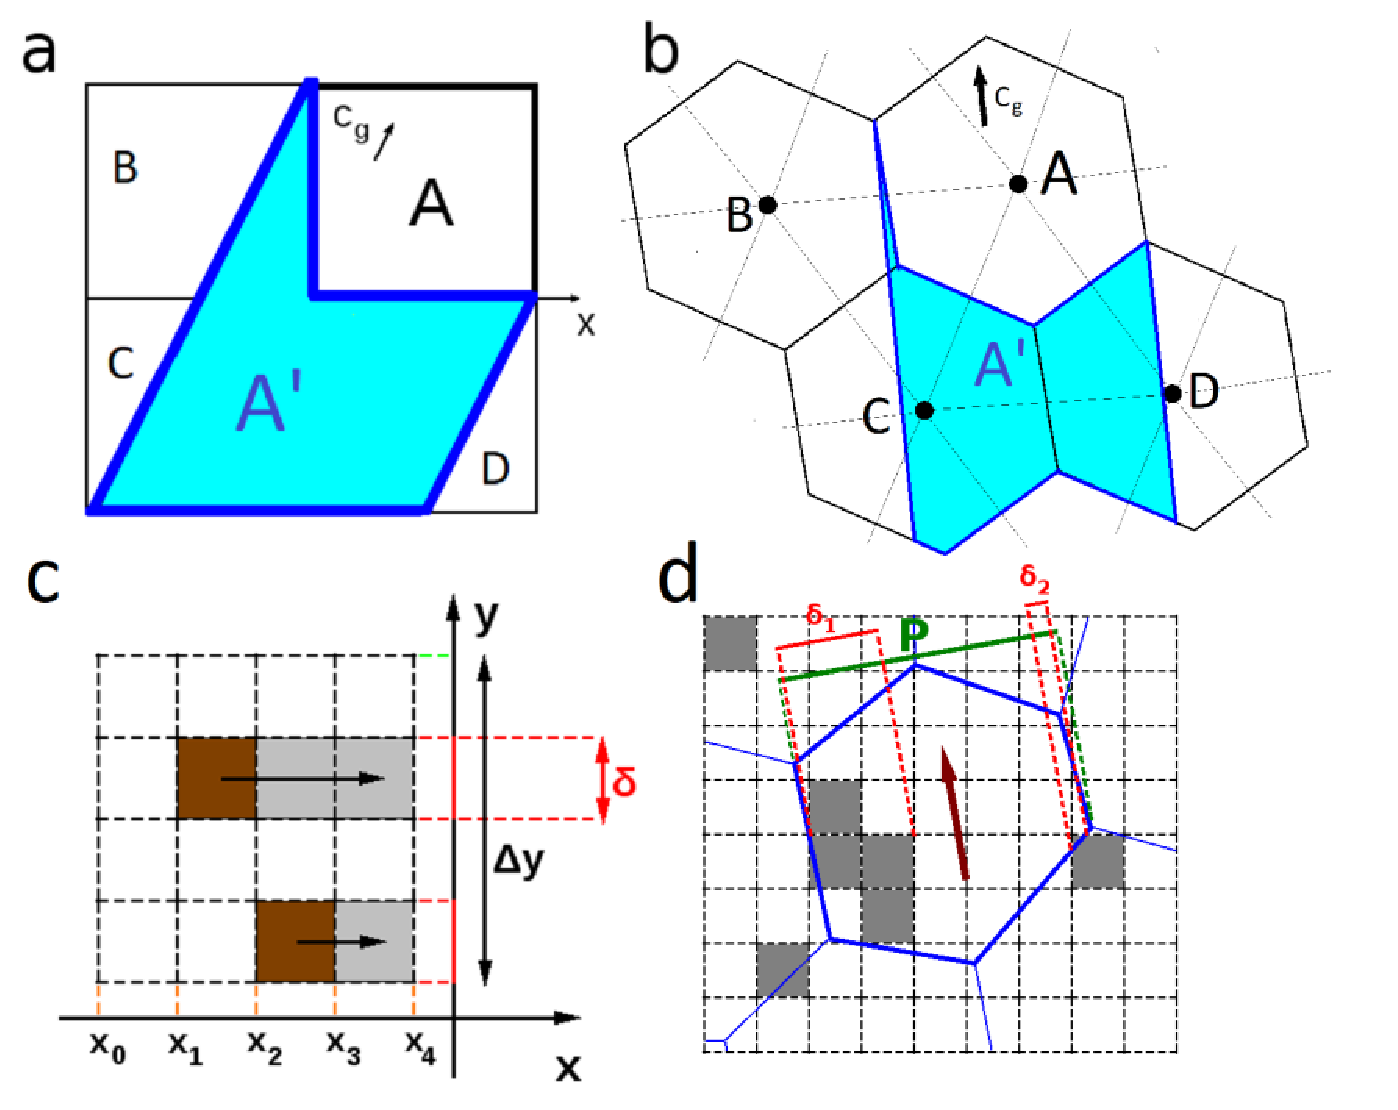
\epsfig{file=./eqs/UOST.eps,angle=0,width=4in}
\caption{
a: a square cell (A) and its upstream polygon 
(A\textsc{\char13}, delimited by blue line, in light blue color) for a spectral 
component propagating with group velocity $c_g$. 
The joint BCD polygon represents the neighborhood polygon. 
b: same as a, but for a triangular mesh (the hexagons approximate the median dual cells). 
c: Computation of $\alpha$ and $\beta$ for a square cell, $N_s=4$, 
and a spectral component propagating along the x axis. 
d: Like c, but for a hexagonal cell and for a tilted spectral component. 
In panel d the gray squares represent unresolved obstacles. 
}
\label{fig:UOST} \botline
\end{center}
\end{figure}


\textbf{Automatic generation of mesh parameters.} 
An open-source python package (alphaBetaLab, https://github.com/menta78/alphaBetaLab) 
was developed
for the automatic estimation, from real-world bathymetry, of the upstream polygons, 
of the transparency coefficients
$\alpha_l$, $\beta_l$, $\alpha_u$, $\beta_u$,
and of the other parameters needed by UOST.
alphaBetaLab considers the cells as free polygons, and estimates the transparency coefficients
from the cross section of the unresolved obstacles versus the incident spectral component 
(figure \ref{fig:UOST}cd).
This involves, that it can be applied to any type of mesh, 
including unstructured triangular and SMC meshes 
(as of August 2018 only regular and triangular meshes are handled, 
but support for SMC meshes 
will be soon added). 
We need to mention that while UOST would be able to modulate the energy dissipation 
with the spectral frequency, only the direction is currently considered in alphaBetaLab.
For more details on the algorithms implemented in alphaBetaLab, 
the user is referred to \cite{art:Mentaschi2018a}. 
\cite{art:Mentaschi2018c} provides the documentation of the software and of its architecture,
along with use guidance and illustrative examples. 

\textbf{Time step settings.} 
In \ws\ the source terms are applied at the end of each global time step.
Therefore, to work properly on a given cell, 
UOST needs a global time step lower
or equal to the critical CFL time step of the cell, 
i.e., the amount of time needed by the fastest spectral component to entirely cross the cell.
Otherwise, part of the energy will leak through the cell without being blocked \citep{art:Mentaschi2018a}.

In unstructured grids with cells of very different sizes, the application of UOST to 
all the cells, including the smallest ones, may come with an excedingly small global time step
that would affect the economy of the model. 
To avoid this problem the user can set alphaBetaLab in order to
neglect cells smaller than a user-defined threshold, and then set in \ws\
a global time step equal to the critical CFL time step related with that threshold 
\citep{art:Mentaschi2018c}.


\begin{table} \begin{center}
 \footnotesize
\begin{tabular}{|p{4cm}|p{2.5cm}|p{5.5cm}|} \hline \hline
Namelist parameter    &  Description           & default value \\
\hline
  UOSTFILELOCAL &  Local $\alpha$/$\beta$ input file path   &  obstructions\_local.\textit{gridname}.in    \\ \hline
  UOSTFILESHADOW &  Shadow $\alpha$/$\beta$ input file path   & obstructions\_shadow.\textit{gridname}.in   \\ \hline
  UOSTFACTORLOCAL &  Calibration factor for local transparencies  &  1   \\ \hline
  UOSTFACTORSHADOW &  Calibration factor for shadow transparencies  &  1  \\
\hline
\end{tabular} \end{center}
\caption{UOST parameters, their description and default values. } \label{tab:UOST}
\botline
\end{table}


\vsssub
\subsubsection{~$S_{xx}$: User defined} \label{sec:XXx}
\vsssub

\opthead{XXn}{---}{user}

\noindent 
This slot is intended for a source term that is not yet classified in
Eq.~(\ref{eq:general_st}). Almost by definition, it cannot be provided here.
\vssub
\subsection{~Source terms for wave-ice interactions}
\vsssub


Wave-ice interaction processes have been the topic of many investigations. In general, wave-ice interactions require 
a description of the ice properties that usually include at least the ice concentration (fraction of ocean surface covered by ice), 
mean ice thickness, and maximum floe diameter. Indeed, the ice is often broken into pieces (the floes) that can have a wide variety of sizes, 
and these sizes strongly modify the dispersion and wave-ice interaction processes. 

In the present version of \ww, the different options 
for treating the ice represent ongoing research. There are now five different 
versions of dissipation processes activated with the switches {\code IC1}, {\code IC2},  {\code IC3}, {\code IC4} and {\code IC5} that can be combined with two 
different versions of scattering effects  {\code IS1} and {\code IS2}. The second scattering routine, because it was the only routine 
to use a maximum floe diameter, also contains an estimation of 
ice break-up and resulting maximum floe diameter and some dissipation due to hysteresis. 

Some features of these switch selections require care in application. For example, other than ice concetration and thickness, the forcing fields are context-based: they take different meanings for different source terms.

At present it is not possible to combine dissipation parametrizations designed for frazil or pancake ice ({\code IC3} or {\code IC4}) with a parametrization designed for the ice pack, such as {\code IC2}. Further, all parameterizations are not yet fully integrated: for example the floe size is not yet taken into account in some modified dispersion relations that take into account the ice. We expect to have a more streamlined way of combining various processes in future versions of \ws, possibly using a maximum floe diameter to call one or the other routines. 

In most cases, \ws\ now permits spatial and temporal variability of ice-related inputs, but in practice this information is usually available only for ice concentration (from satellite or model) and thickness (most often from a model). The variability of other parameters representing the nature of the sea ice is rarely available to the user. 

Observational study of effects of sea ice on waves are challenging, and the modeling of these effects in and near the ice edge is particularly difficult, where the accuracy of the non-stationary and non-uniform input ice fields can be a primary limition on accuracy \citep{rep:RPLA18}. A number of important modeling studies use models other than \ws, e.g. \cite{art:DB13}. So far, the various options available in \ws\ and described in the following sections have been tested in real conditions in a handful of studies, including \cite{art:LKS15}, \cite{art:Aea16}, \cite{art:WHR16}, \cite{art:RTS16}, \cite{rep:RPLA18}, \cite{art:CRT17}, and \cite{Liu2020}.

% Note: IC2 dispersion relation equation was moved to IC2 section

\noindent
Experimental routines for representation of the effect of ice on waves have
been implemented using the switches {\code IC1}, {\code IC2}, {\code IC3}, etc. The first two implemented in \ws\ (by \cite{rep:RO13}), were {\code IC1} and the initial version of {\code IC2} which was based on the work by \cite{art:LMC88} and \cite{art:LHV91}. These effects can be presented in terms of a complex wavenumber

\begin{equation}\label{eq:waveno}
     {k} = {k_r} + i{k_i},
\end{equation}

\noindent
with the real part ${k_r}$ representing impact of the sea ice on the physical
wavelength and propagation speeds, producing effects analogous to shoaling and
refraction by bathymetry, whereas the imaginary part of the complex
wavenumber, ${k_i}$, is an exponential decay coefficient
${k_i}({x},{y},{t},\sigma $) (depending on location, time and frequency,
respectively), producing wave attenuation.  The ${k_i}$ is introduced as
${S_{ice}}/{E}=-2{c_g}{k_i}$, where ${S_{ice}}$ is a source term (see also
\cite{bk:WAM94}, pg. 170).  With the methods that provide  ${k_r}$, e.g. {\code IC2}, 
{\code IC3}, and {\code IC5}, the sea ice effects 
require solution of a new dispersion relation.

The effect of sea ice on ${k_i}$ is used for all source functions in \ws\ version 6:
{\code IC1}, ..., {\code IC5}. The effect of sea ice on ${k_r}$ has
been implemented for {\code IC2} and {\code IC3}, but is exported for use in
the rest of the code only for {\code IC3}, and this remains an experimental feature.

% Note : Is the above still true? Has it been done for IC2 now also?

The ice source functions are scaled by ice concentration.

In the case of ice, up to five input parameters are allowed as 
non-stationary and non-uniform fields. These can be referred
to generically as ${C_{ice,1}}$, ${C_{ice,2}}$, ..., ${C_{ice,5}}$.  The meaning
of the ice parameters will vary depending on which ${S_{ice}}$ routine is
selected. For example, in case of {\code IC1}, only one parameter is specified, ${C_{ice,1}}$.
In some cases, e.g. {\code IC3} and {\code IC4}, there are options for taking the simpler approach
of inputting the same variables as stationary and uniform, defined using namelist parameters.

The reader is referred to the regression tests {\file ww3\_tic1.1-3} and
{\file ww3\_tic2.1} for examples of how to use the new ice source functions.

\textrm{\textit{\underline{Use within {\file ww3\_shel}:}}} 
Non-stationary and non-uniform input ice parameters are permitted.
In the case where any of the ice and mud source functions are activated with
the switches {\code IC1}, {\code IC2}, {\code IC3}, {\code IC5}, {\code BT8}, or {\code
BT9}, {\file ww3\_shel} will anticipate intructions for 8 fields (5 for ice,
then 3 for mud). These are given prior to the ``water levels'' information.
The new fields can optionally be specified as a homogeneous field using lines
found near the end of {\file ww3\_shel.inp}. 

\textrm{\textit{\underline{Use within {\file ww3\_multi} (New in \ws\ version 6):}}} Using the namelist method of
providing instructions to {\file ww3\_multi}, it is now possible to prescribe mud and ice coefficients as non-stationary and non-uniform fields in {\file ww3\_multi}. Prior to version 6, this was only possible with {\file ww3\_shel}. 
However, the new method of reading these instructions via {\file ww3\_multi.nml} has not yet been tested by this author at time of writing.

\textrm{\textit{\underline{Separation of the source terms:}}} 
The source terms {\code IC1},...,{\code IC5} predict dissipation of wave energy. The reflection and scattering of waves from sea ice  (e.g. \cite{art:Wad75}) are not dissipation: they are conservative processes. They are treated separately in {\code IS1} and {\code IS2}.

\vsssub
\subsubsection{~$S_{ice}$: Damping by sea ice (simple)} \label{sec:ICE1}
\vsssub

\opthead{IC1}{\ws/NRL}{E. Rogers and S. Zieger}

The first implemented method ({\code IC1}) is for the user to specify
${k_i(x,t)}$, which is uniform in frequency space, ${C_{ice,1}}={k_i}$. The
parameters ${C_{ice,2}}$,...,${C_{ice,5}}$ are not used. An example setting
is ${C_{ice,1}}=2\times 10^{-5}$. Descriptions specific to {\code IC2} and {\code IC3} are
given in following sections. 

A full description of {\code IC1} can be found in \cite{rep:RO13} and a concise summary is given in \cite{rep:RPLA18}. This simple method was applied in \cite{art:LKS15} and is used as the modeling component of a model-data inversion procedure by \cite{art:RTS16}, \cite{rep:RPLA18}, and \cite{rep:RMK18}.

\vsssub
\subsubsection{~$S_{ice}$: Damping by sea ice (Liu et al.)} \label{sec:ICE2}
\vsssub

\opthead{IC2}{\ws/NRL}{E. Rogers, S. Zieger, F. Ardhuin}

\noindent
This method for representing the dissipation of wave energy by wave-ice interaction is based on the papers
by \cite{art:LMC88}, \cite{art:LHV91} and \cite{art:Aea15}. The main input ice parameters
is the ice thickness (in meters) that can vary spatially and temporally and is the forcing field  ${C_{ice,1}}$. 

This is a model for attenuation by a
sea ice cover, derived on the assumption that dissipation is caused by
friction in the boundary layer below the ice,
with the ice modeled as a continuous thin elastic plate. The original form by  \cite{art:LMC88} is activated by 
setting the {\code IC2} namelist {\F SIC2} parameter {\code IC2DISPER = .TRUE.}. That form 
 assumes that the boundary layer is always laminar but it uses an eddy viscosity ${\nu}$ that can vary spatially 
and is the forcing field ${C_{ice,2}}$. 

 {\code IC2} and {\code IS2} share 
the optional use of the \cite{art:LMC88} dispersion relation for unbroken ice, 
\begin{equation}
\sigma^2 =  \left(gk_{ice} + B k_{ice}^5\right)  / \left(1/\tanh ( k_{ice}H) +\frac{\rho_{ice}  h k_{ice}} {\rho_{w} }\right),
\end{equation}
\begin{equation}
c_g =  (g+(5 + 4 k_{ice} M)Bk_{ice}^5)/(2\sigma(1+k_{ice}M)^2).
\end{equation}

\noindent
$B$ and $M$ quantify the effects of, respectively, ice bending due to waves and ice inertia. 
The group velocity under the ice, derived from the same relation, is used in the module {\code W3SIS2MD} and computed in  
{\code W3DISPMD}.  See \citet{art:LMC88} for details.

For {\code IC2}, the dispersion relation is defined by 

\begin{equation}\label{eq:ice1}
  {\sigma}^2 = ({gk_r} + {Bk_r^5})/(\coth({k_r}{h_w}) + {k_r}{M}),
\end{equation}
\begin{equation}\label{eq:ice2}
  {c_g} = (g + (5 + 4{k_r}{M}){B}{k_r^5})/(2{\sigma}(1+{k_r}{M})^2),
\end{equation}
\begin{equation}\label{eq:ice3}
  {\alpha} = (\sqrt{{\nu\sigma}}{k_r)}/({c_g}\sqrt{2}(1+{k_r}{M})).
\end{equation}

\noindent
In our notation, $h_w$ is water depth and $h_i$ is ice thickness.  The
variables $B$ and $M$ quantify the effects of the bending of the ice and
inertia of the ice, respectively. Both of these variables depend on $h_i$ 
\citep[see][]{art:LMC88, art:LHV91}.

This equation is only solved when ICEDISP=TRUE in the {\F MISC} namelist. Otherwise, $k_{ice}=k$, just like in open water. 
Note that the effect of $k_{ice}$ is not passed back to the main program. 
% I temporarily removed text "...is limited to wave breaking and dissipation..." : is this true? Or did the author mean to say "ice breaking and dissipation"? 

 \cite{art:SAG16} improved {\code IC2} by adding a better alternative to the eddy viscosity representation of dissipation. 
They distinguish between laminar and 
turbulent regimes, allowing this is activated by setting  {\code IC2DISPER = .FALSE.}. 
In that case the dissipation goes from a laminar form using the molecular viscosity multiplied by an 
empirical adjustment factor {\code IC2VISC} to a turbulent form, amplified by a factor {\code IC2TURB}, for Reynolds numbers 
above a user-defined threshold {\code IC2REYNOLDS}. This transition is smoothed over a range {\code IC2SMOOTH} to take into 
account the random nature of the wave field. In the turbulent regime, the friction factor 
is estimated from a user-specified under-ice roughness length {\code IC2ROUGH}, expected to be of the order of $10^{-4}$~m. 
Possibility has also been added to perform a heuristic reduction of the dissipation 
rate when the floe diameters are much shorter than the ocean wave 
wavelength \citep[see][for details]{Aea18}. It relies on the hypothesis that, in these conditions, ice floes follow at least partly 
the horizontal motion and it is thus logical to reduce the relative velocity 
between the ice and the water from which the dissipation rate is estimated. 
This reduction is controlled by the factor called $r_D$ in \cite{Aea18} which value can be set through the namelist parameter {\code IC2DMAX}. 
Reduction of the dissipation rate occures for waves longer than $D_{\max}/r_D$ ($D_{\max}$ 
being the maximum floe size), and there is no reduction for maximum floe diameters of the order of 
the wavelength or more.

The parameter {\code IC2TURBS} is an ad hoc enhancement of turbulent dissipation in the Southern hemisphere 
that was introduced for test purposes to investigate sources of bias. This will be deprecated in future versions. It now appears 
that combining IC2 with ineleastic dissipation in IS2 can provide good results for dominant waves in both hemispheres \citep{Aea18}. 

A full description of the original form of {\code IC2} can be found in \cite{rep:RO13}. 
It is applied in \cite{art:LKS15}. A concise summary of the present code is given 
in \cite{rep:RPLA18}. A description of the improvement of the dissipation mechanism 
of {\code IC2} can be found in Appendix B of \cite{art:SAG16}, where it is used.

\vsssub
\subsubsection{~$S_{ice}$: Damping by sea ice (Shen et al.)} \label{sec:ICE3}
\vsssub

\opthead{IC3}{Clarkson U. Fortran-77 code}{E. Rogers, X. Zhao, S. Cheng, S. Zieger}

\noindent
The third method for representing wave-ice interactions is taken from\linebreak
\cite{art:WS10}. This model treats the ice as a visco-elastic
layer. ${C_{ice,1}}$ is used for ice thickness (m); ${C_{ice,2}}$ is used for
the viscosity ($\mathrm{m^2\,s^{-1}}$); ${C_{ice,3}}$ is used for density
($\mathrm{kg\,m^{-3}}$); ${C_{ice,4}}$ is used for effective shear modulus
(Pa); ${C_{ice,5}}$ is not used. An example setting is 
${C_{ice,1...4}}=[0.1, 1.0, 917.0, 0.0]$.

In \ws\ version 4, this method of $S_{ice}$ ({\code IC3}) was much more expensive than {\code IC1} or {\code IC2}. This issue is largely addressed in model version 5.16.

The namelist {\F SIC3} is introduced in model version 5.16. The namelist parameters are summarized in a list here, and some are discussed in further detail below.

\begin{clist}
\cit {IC3CHENG} {Solution technique new in version 5.16. Default = {\code TRUE}.}
\cit {IC3HILIM} {Optional limiter on ice thickness. Default=100 (i.e. by default, the option is not used).}
\cit {IC3KILIM} {Optional limiter on dissipation rate ${k_i}$. Default=100 (i.e. by default, the option is not used).}
\cit {USECGICE} {When set to {\code TRUE}, the model will include the effect of ice on the group velocity. Default = {\code FALSE}.}
\cit {IC3VISC} {If user wishes to use an effective viscosity that is constant and uniform, this can now be done via namelist. Default=N/A.}
\cit {IC3ELAS} {As with {\code IC3VISC}, but for effective elasticity. Default=N/A.}
\cit {IC3DENS} {As with {\code IC3VISC}, but for ice density. Default=N/A.}
\cit {IC3HICE} {As with {\code IC3VISC}, but for ice thickness. Default=N/A.}
\cit {IC3MAXCNC} {Parameter which can be used to optionally switch to another dissipation for some ice conditions (see below). Default=100 (i.e. option is not used). Normal range is 0 to 1.}
\cit {IC3MAXTHK} {Idem. Default=100 (i.e. option is not used). Normal range is 0 to 10 meters.}        
\cit {IC2REYNOLDS} {Parameter associated with IC2 non-dispersive turbulent boundary layer scheme. Default=1.5e+5.}
\cit {IC2ROUGH} {Idem. Default=0.02.}
\cit {IC2SMOOTH} {Idem. Default=7.0e+4.}
\cit {IC2VISC} {Idem. Default=2.0.}
\cit {IC2TURB} {Idem. Default=2.0.}          
\cit {IC2TURBS} {Idem. Default=0.0.}
\end{clist}

The {\code IC3CHENG} option is new in model version 5. When set to {\code TRUE}, the model will use an alternative solution technique provided by S. Cheng. This has two important features. First, stability is improved, such that there is no need to use the ice limiter, i.e. the {\code IC3HILIM} parameter. Second, this method requires that three of four ice rheology parameters be stationary and uniform, input via namelist parameters (see below).

If {\code IC3CHENG} is set to {\code FALSE}, the user is advised to use the ice thickness limiter {\code IC3HILIM} to ensure stability (value of 25 to 100 cm is suggested). The parameter {\code IC3KILIM} was required for stable and fast computations in some prior development versions of \ws, but is now unnecessary and may be ignored by the user.

In model version 4.18, four ice rheology parameters (ice thickness, effective viscosity, effective elasticity, and ice density) were allowed to be nonstationary and non-uniform. This could be provided using {\file ww3\_prep}. Or in cases where {\file ww3\_shel} is used and non-uniform inputs are unnecessary, the ``homogeneous'' option of {\file ww3\_shel} was available for rheology input. In model version 5.16, an option is added to specify the four ice rheology parameters via the namelist {\F SIC3}. Two restrictions apply: 1) If {\code IC3CHENG} is set to {\code FALSE} and  {\code USECGICE} is set to {\code TRUE}, the namelist method cannot be used, and 2) If {\code IC3CHENG} is set to {\code TRUE}, the namelist method must be used for three of the rheology parameters (effective viscosity, effective elasticity, and ice density). If {\code IC3CHENG} is set to {\code TRUE} or {\code USECGICE} is set to {\code FALSE}, the fourth ice rheology parameter (ice thickness) can be input by either method (namelist or non-namelist). The model performs error checking to ensure that the user has specified input for each parameter by a single method (neither method of input is assumed to supercede the other).

The ${k_r}$ modified by ice is incorporated into the governing
equation~(\ref{eq:bal_plane}) via the $c_g$ (group velocity) and $c$ (phase velocity) calculations on the
left-hand side; e.g. \citet[][and subsequent unpublished work]{art:RH09}. 
The modification of wavenumber and group velocity can be optionally passed back to the main program to produce effects analogous to refraction and shoaling by bathymetry. However, this feature has been used so far only in academic studies, rather than in routine application to realistic scenarios.\\

To activate the shoaling effect, the model should be
operated with namelist variable {\code USECGICE = TRUE}. To activate the refraction effect, the model should be
compiled with switch {\code REFRX}. With this switch, the model computes
refraction based on spatial gradients in phase velocity that include ice effects, rather than the
simpler wave dispersion relation without ice. These effects are demonstrated in the regression test {\file
ww3\_tic1.3} which is provided with the code.

The group velocity using {\code IC3CHENG} solver with zero ice thickness does not collapse exactly to that from the open water dispersion relation. This is caused by numerical error in the calculation $c_g = \frac{\partial \sigma}{\partial k} = \frac{\Delta \sigma}{\Delta k} $. These small differences in group speed will result in slight shoaling and refraction errors if these effects are turned on. Error for ice thickness equal to zero was found less than 10\% and frequency dependent. This has been avoided by skipping the solver if ice thickness is exactly zero. If ice thickness is close to but not exactly zero, then this discrepancy may be noticeable. The solutions from CHENG for other parameters (effective viscosity, effective shear modulus) as they approach zero were not tested. Small but material difference have also noted between the solutions from {\code IC3CHENG} set to {\code FALSE} vs. {\code TRUE} for the same ice inputs.

As noted above, {\code USECGICE = TRUE} is required for the shoaling effect. However, since some ice rheology will lead to an increase in group velocity, the user is advised to use care with this option. The group velocity affects the CFL criterion, which may require that the user reduce the time step size. {\code USECGICE = FALSE} is recommended for users that do not wish to worry about this issue.

In model version 5.16, a non-default option is added which causes the dissipation parameterization to change for some ice conditions. If ice concentration exceeds {\code IC3MAXCNC} and ice thickness exceeds {\code IC3MAXTHK}, the {\code IC2} dissipation (more specifically, the non-default, non-dispersive boundary layer scheme sub-option of {\code IC2}) is used in place of the dispersion-based dissipation estimate of \cite{art:WS10}. See description of {\code IC2} for more information. Since it is non-dispersive, this feature should not be used with {\code USECGICE = TRUE}.

{\code IC3} first appeared in \ww\ version 4 and the first simple testing was reported in \cite{pro:RZ14}. It has since been used in \cite{art:LKS15}, \cite{art:WHR16}, \cite{art:RTS16}, and \cite{art:CRT17}.

\vsssub
\subsubsection{~$S_{ice}$: Empirical/parametric damping by sea ice} \label{sec:ICE4}
\vsssub

\opthead{IC4}{\ws/NRL}{C. Collins and E. Rogers}

\noindent
The fourth option ({\code IC4}) for damping of waves by sea ice was introduced by \cite{rep:CR17}. It gives methods to implement one of several simple, empirical/parametric forms for the dissipation of wave energy by sea ice.  The motivation for {\code IC4} is to provide a simple, flexible, and efficient source term which reproduces, albeit in a highly parameterized way, some basic physics of wave-ice interaction. The method is set by the integer value (presently 1 to 7) for {\code IC4METHOD} namelist parameter: 1) an exponential fit to the field data of \cite{art:WAD88}, 2) the polynomial fit in \cite{art:MBK14}, 3) a quadratic fit to the calculations of \cite{art:KM08} given in \cite{art:HT15}, 4) Eq. 1 of \cite{art:Ko14}, 5) a simple step function with up to 4 steps (may be nonstationary and non-uniform), and 6) a simple step function with up to 10 steps (must be stationary and uniform), and 7) a formula from \cite{art:Dob15} which uses ice thickness. All but the fourth method of {\code IC4} feature frequency-dependent attenuation. With the fourth method, attenuation varies with waveheight but is uniform in frequency space. 

In the following discussion we use {\code IC4M1} to denote {\code IC4} method 1, and so forth. {\code IC4} appears in the {\file switch} and namelist {\code IC4METHOD=1} (for example) appears in the file {\file ww3\_grid.inp}. Whereas in {\code IC1}, ${C_{ice,1}}$ is the user-determined attenuation, for {\code IC4M1}, {\code IC4M2}, and {\code IC4M4} ${C_{ice,n}}$ are constants of the equations. For {\code IC4M3}, ${C_{ice,1}}$ is ice thickness. For {\code IC4M5}, ${C_{ice,n}}$ controls the step function. Note that ${C_{ice,n}}$ may be provided by the user as non-stationary and non-uniform using methods analogous to methods used to input water levels.

{\code IC4M1}: an exponential equation was chosen to fit the data contained in table 2 of \cite{art:WAD88} which results in preferential attenuation of high frequency waves. This parameterizes the well-known low-pass filtering effect of ice. The equation has the following form:
\begin{equation}\label{eq:ice1}
  {\alpha} = \exp\left[\frac{-{2\pi}C_{ice, 1}}{{\sigma}} - C_{ice, 2}\right]
\end{equation}

\noindent Here, $\alpha$ is the exponential decay rate for energy, which is twice that for amplitude: $\alpha = 2k_i$. The values determined from the data are ${C_{ice,1...2}}=[0.18, 7.3]$, but these may be modified by the user. This method is described and applied in \cite{rep:CR17}.

{\code IC4M2}: In this method, the dissipation is represented using a user-specified polynomial. It is a powerful method, since many shapes can be represented, e.g. by fitting to observation-based dissipation rates. The method is described and applied in \cite{rep:CR17}. The equation is the following:
\begin{equation}\label{eq:ice2}
  {\alpha} = C_{ice,1} + C_{ice,2}\left[{\frac{\sigma}{2\pi}}\right] + C_{ice,3}\left[{\frac{\sigma}{2\pi}}\right]^2 + C_{ice,4}\left[{\frac{\sigma}{2\pi}}\right]^3 + C_{ice,5}\left[{\frac{\sigma}{2\pi}}\right]^4
\end{equation}

\noindent
If a user wishes to follow \cite{art:MBK14}, the suggested values for the coefficients are ${C_{ice,1...5}}=[0, 0, 2.12\times 10^{-3}, 0, 4.59\times 10^{-2}]$. Additional suggested polynomials can be found in \cite{rep:RMK18}.

With appropriate coefficients, this polynomial method can be used to reproduce the so-called “roll-over effect” where the attenuation is non-monotonic in frequency space. However, some recent studies do not indicate this effect, e.g. \cite{art:RTS16} and \cite{art:LK17}, and it may just be a spurious artifact in prior observational studies.

{\code IC4M3}: \cite{art:HT15} fit a quadratic equation to the attenuation coefficient calculated by \cite{art:KM08} as a function of frequency, $T$, and ice thickness, $h$. Attenuation increases for thicker ice and higher frequencies (lower periods). The number of  coefficients of the quadratic equation were prohibitively large to be user-determined, so the equation is hardwired in and the tunable parameter, ${C_{ice,1}}$, is ice thickness $h$. This method is described and applied in \cite{rep:CR17}. For reference, the equation is the following:
\begin{equation}\label{eq:ice3}
  {\ln{\alpha(T,h)}} = -0.3203 + 2.058h - 0.9375T - 0.4269h^2 + 0.1566hT + 0.0006T^2
\end{equation}

\noindent
There are two warnings to make about {\code IC4M3}. First, the equation itself was an extrapolation of the original range of $h$ used to calculate the attenuation coefficients in \cite{art:KM08} which was between 0.5 and 3 m, see \cite{art:HT15}. Second, in \cite{art:KM08}, wave attenuation predicted is based on scattering (a conservative process), whereas in {\code IC4M3}, the wave attenuation is treated as dissipation (non-conservative). This is ad hoc and not recommended for general use. Most especially, users should think twice before using {\code IC4M3} in combination with scattering routines {\code IS1} or {\code IS2}, since this is essentially double-counting scattering.

{\code IC4M4}: \cite{art:Ko14} found that attenuation was a function of significant wave height. Attenuation increased linearly with ${H_s}$ until ${H_s} = 3$ m at which point attenuation is capped, thus:
\begin{equation}
\left \{
\begin{array}{llrcl}
{\frac{\partial H_s}{\partial dx}} = {C_{ice,1}}\times {H_s}   & & \text{for} \> {H_s} \leq 3 \text{ m}  \\
{\frac{\partial H_s}{\partial dx}} = {C_{ice,2}}               & & \text{for} \> {H_s} > 3 \text{ m}     \\
\end{array} \right .
\end{equation}
where {$k_i=\frac{\partial H_s}{\partial dx}/H_s$}.

The values given in \cite{art:Ko14} are ${C_{ice,1...2}}=[5.35\times 10^{-6}, 16.05\times 10^{-6}]$. See regression test {\file ww3\_tic1.1/input\_IC4/M4} for examples. This method is described and applied in \cite{rep:CR17}.

{\code IC4M5}: This is a simple step function with up to 4 steps. It is controlled by the optionally nonstationary and non-uniform parameters ${C_{ice,1...7}}$. Parameters ${C_{ice,1...4}}$ control the step levels, which are in terms of dissipation rate, ${k_i}$. Parameters ${C_{ice,5...7}}$ control the step boundaries (given in Hz). See regression test {\file ww3\_tic1.1/input\_IC4/M5} for examples. This method is described in \cite{rep:CR17}.

{\code IC4M6}: This is a simple step function with up to 10 steps. It is controlled by the stationary and uniform namelist parameters {\code IC4KI} and {\code IC4FC}. Array {\code IC4KI} controls the step levels, which are in terms of dissipation rate, ${k_i}$, in radians per meter. Array {\code IC4FC} controls the step boundaries (given in Hz). See regression test {\file ww3\_tic1.1/input\_IC4/M6} for examples. 

{\code IC4M7}: This is a formula for dissipation from \cite{art:Dob15}, developed for a mixture of pancake and frazil ice, using data collected in the Weddell Sea (Antarctica). The formula depends on wave frequency and ice thickness:
\begin{equation}\label{eq:ice7}
  {\alpha=0.2T^{-2.13}h} \:\:\: .
\end{equation}
This method is described in \cite{rep:RPLA18}.

\vsssub
\subsubsection{~$S_{ice}$: Damping by sea ice (Mosig et al.)} \label{sec:ICE5}
\vsssub

\opthead{IC5}{U. of Otago MATLAB code}{Q. Liu, E. Rogers, A. Babanin}

\noindent
The fifth method for representing ice-induced wave decay is based on another viscoelastic-type model, i.e., the EFS ice layer model described in \citet{art:MMS15}. The authors introduced viscosity into the thin elastic plate model of \citet{art:FS1994} and restricted it to one horizontal dimension (replacing a plate by a beam). The dispersion relation given by the EFS model can be written in the form
\begin{equation}
Q g k \tanh(k d)-\sigma^2 = 0,
\label{eq:ic5a}
\end{equation}
%
\begin{equation}
Q = \frac{G_{\eta} h_i^3}{6 \rho_w g} (1+\nu) k^4 - \frac{\rho_i h_i \sigma^2}{\rho_w g} + 1.
\label{eq:ic5b}
\end{equation}
%
In Eq.~(\ref{eq:ic5a})$-$(\ref{eq:ic5b}), $G_{\eta} = G - i \sigma \rho_i \eta$ is the complex shear modulus, where $G$ is the \emph{effective} elastic shear modulus and $\eta$ is the \emph{effective} viscosity; $\rho_w$ ($\rho_i$) is the density of water (ice), $d$ is water depth, $h_i$ is the ice cover thickness, $\sigma$ is the radian frequency, $k=k_r + i k_i$ is the complex wavenumber, $g$ is the gravitational acceleration and $\nu=0.3$ refers to the Poisson ratio of sea ice.

Same as {\code IC3}, {\code IC5} requires four ice parameters as input: $C_{ice, 1}$ for ice thickness $h_i$ (m), $C_{ice, 2}$ for the \emph{effective} viscosity $\eta$ (m$^2$ s$^{-1}$), $C_{ice, 3}$ for ice density $\rho_i$ (kg m$^{-3}$) and $C_{ice, 4}$ for the \emph{effective} shear modulus $G$ (Pa). For example, as shown in \citet[][see their Fig. 8]{art:MMS15}, a setting of $C_{ice, 1,...,4}=[1.0\ \mathrm{m},\ 5.0\times10^7\ \mathrm{m^2\ s^{-1}},\ 917.0\ \mathrm{kg\ m^{-3}},\ 4.9\times10^{12}\ \mathrm{Pa}]$ (with a water depth $d$ of 4300 m) can be used to fit the observed wave attenuation rates reported in \citet{art:MBK14}. The application of the EFS model to two realistic case studies is presented in \citet{Liu2018ic5}.

The dispersion relation shown above is solved iteratively using the Newton-Raphson method. The numerical solver, however, may fail for small wave periods in some rare cases (particularly for shallow water depth $d$ and low $G$). In such cases, the estimated wavelength $k_r$ is unreasonably low. Several namelist variables (limiters) are introduced to improve the code stability:
\begin{clist}
\cit{IC5MINIG} {the minimum allowed shear modulus $G$; Default= 1 Pa (i.e., zero $G$ is not allowed).}
%
\cit{IC5MINWT} {the minimum allowed wave periods $T$; Default=0 s (i.e., by default, this option is not used).}
%
\cit{IC5MAXKRATIO} {the maximum allowed $k_{ow}/k_r$, where $k_{ow}$ is the open-water wavenumber; Default=1E9 (i.e., by default, this option is not used).}
%
\cit{IC5MAXKI} {the maximum allowed $k_i$; Default=100 m$^{-1}$ (i.e., by default, this option is not used).}
%
\cit{IC5MINHW} {the minimum allowed water depth $d$; Default=300 m (this basically limits {\code IC5} to the deep-water case).}
%
\cit{IC5MAXITER} {the maximum allowed \# of iteration; Default=100.}
\end{clist}

Note that the EFS model used here regards the ice cover as a continuous homogeneous medium and characterizes various ice types with two \emph{totally empirical} rheological parameters, namely the elastic shear modulus $G$ and the viscosity $\eta$. As argued in \citet{art:MMS15}, these two parameters \emph{``cannot be measured directly as they do not represent observable physical processes''}. Therefore, ``no restrictions on the acceptable values of the rheological parameters, \emph{except positiveness}, can be imposed.'' So strictly speaking, the EFS model is better termed as an \emph{effective medium} model rather than a \emph{viscoelastic} model.

\vsssub
\subsubsection{~$S_{is}$: Diffusive scattering by sea ice (simple)} \label{sec:IS1}
\vsssub

\opthead{IS1}{\ws/NRL}{S. Zieger}

\noindent
The non-conservative effect of ice on waves has been implemented in switches
{\code IC1} through {\code IC3} (see \para\ref{sec:ICE1}--\ref{sec:ICE3}). The
conservative effect of sea ice has been implemented in switch {\code IS1} and
represents a simple form of scattering. It is assumed that the floe size is
smaller than the grid size and that a fraction $\alpha_{ice}$ of the incoming
wave energy is scattered isotropically. The fraction is determined from sea ice
concentration ICE using a simple linear transfer function
\begin{equation}\label{eq:IS101}
     \alpha_{ice} = \max\left \{0 , C_1\ \mathrm{ICE} + C_2 \right \} \:\:\: .
\end{equation}

\noindent
The coefficients $C_1$ and $C_2$ are customizable through namelist {\F SIS1}
with namelist parameters {\code ISC1} and {\code ISC2}. At each discrete
frequency and direction the wave energy is reduced by the amount of
$\alpha_{ice}$ and redistributed to all direction in the same discrete
frequency to conserve energy.



\vsssub
\subsubsection{~$S_{is}$: Floe-size dependent scattering and dissipation} \label{sec:IS2}
\vsssub

\opthead{IS2}{\ws}{F. Ardhuin, C. Sevigny, G. Boutin,  D. Dumont,  T. Williams}


The implementation of this scattering term generally 
follows the approach of \cite{art:MM06}, to which has been added an estimation of the breakup of the ice 
by waves to be able to update a maximum floe size diameter. Finally a creep-based dissipation was also 
combined with the scattering.  


The scattering source term is defined by the scattering coefficient $\beta_{\mathrm{is},\mathrm{MIZ}}(\theta-\theta')$ which by default is isotropic, but can be given any directional dependency by setting {\code IS2ISOSCAT=FALSE} in namelist {\F SIS2}. The source term is thus,
\begin{equation}
 \frac{S_{\mathrm{is}}(k,\theta)}{\sigma} =  \int_0^{2\pi}\beta_{\mathrm{is},\mathrm{MIZ}}(\theta-\theta') [s_\mathrm{scat}  N(k,\theta')-N(k,\theta)] d\theta'  .
 \end{equation}
where $s_\mathrm{scat}$ is set to 1.0 by default but can be modified by 
{\code IS2BACKSCAT} in namelist {\F SIS2}. \\


The determination of scattering coefficients  $\beta_{\mathrm{is},\mathrm{MIZ}}$ is based on the theoretical 
reflection coefficient $\alpha_n(\sigma,h)$
for waves with a normal incidence going from a half-plane of open water to a half-plane of ice-covered water with a 
constant ice thickness $h$.  
Values of $\alpha_n(\sigma,h)$ as computed by \cite{art:KM08}
 (if {\code IS2WIM1=0.}) or by \cite{art:Ben12} (if {\code IS2WIM1=1.})  are tabulated 
in the {\code W3SIS2MD} module. Following \cite{art:Dea11}, the broken ice is treated as a series of 
such ice-water interfaces. Neglecting multiple reflections, the scattering parameterization defines the attenuation 
per unit time as if the ice-covered part of a grid cell was a succession of floes of mean diameter $D_{m}$ with a partial 
reflection $\alpha_n(\sigma,h)$ for each floe, giving, 
\begin{equation}
\beta_{\mathrm{is},\mathrm{MIZ}}=c_i~c_g \alpha_n(\sigma,h) / D_{m},
 \end{equation}
where $c_i$ is the ice concentration. \\
 

The estimation of the mean floe diameter $D_m$ is based on an assumed power law for the number of 
floes of diameter $D$, taken  proportional to $D^{-\gamma}$. This power law is further assumed to 
apply for $D$ ranging from 
the minimum $D_{\min}$ and a maximum $D_{\max}$. The average is thus given by  
\begin{equation}
D_m=\frac{\gamma}{\gamma -1}\times\frac{D_{\max}^{-\gamma +1}-D_{\min}^{-\gamma +1}}{D_{\max}^{-\gamma}-D_{\min}^{-\gamma}}.
\label{analytic_Dbar}
\end{equation}

\noindent
At present $D_{\min}$ is a user-supplied value. $D_{\max}$ can either be 
provided as a forcing field, e.g. from an 
ice model or some observations, or, if the namelist parameter {\code IS2BREAK} is set to {\code TRUE}, 
estimated from 
the breaking of the ice by the local wave field. If the namelist parameter {\code IS2DUPATE}  is set to  
{\code TRUE}, small values of $D_{\max}$ will persist even if the waves become too small to be able to break the ice to 
that size. This is probably the proper model 
use when  external forcing/coupling is available (e.g. advection of ice properties in an ice model). 
 On the contrary, if {\code IS2DUPDATE} is set to  {\code FALSE}, the value of $D_{\max}$ will be always adjusted to the local sea state, 
even if that means increasing $D_{\max}$.\\


Ice breaking by waves of wavelength $\lambda$ is assumed to produce floes of diameter $\lambda / 2$. 
In the parametrization, ice breaking occurs if the three following criteria are fulfilled \citep{art:Wea13}:
\begin{enumerate}
\item $\lambda/2 \geq D_{\min} \quad \mathrm{and} \quad  \lambda/2 \leq D_{\max}$
\item $D_{\max}>D_c$, as it exists a critical diameter, which depends on ice properties, below which no flexural failure is possible
\item $\varepsilon>\varepsilon_c$, the strain due to the incoming wave has to 
be greater than a defined critical strain
\end{enumerate}
The first criterion is simply checking that the new value of $D_{\max}$ will be larger than $D_{\min}$ and smaller 
than the previous value of $D_{\max}$.\\

The second criterion relies on \cite{inc:M86} with the correction specified in \cite{art:Bea18}, where $D_{c}$ is defined as
\begin{equation}
D_{c}=\dfrac{1}{2}\left(\frac{\pi^4 Y^* h^3}{48 \rho g (1 -\nu ^2)}\right)^{1/4}. 
\end{equation}

The third criterion corresponds to the flexural strain threshold. The horizontal 
strain caused by waves is related to 
the curvature of the ice layer, which, in one dimension is 
$\varepsilon = 0.5 h \partial ^2 \eta_{\mathrm ice} / \partial x^2$. 
The strain variance is given 
\begin{equation}
\langle\varepsilon^2\rangle = \left( \frac{h}{2} \right) ^2   \int_{k_1}^{k_2} k_{ice}^4 F(k)dk ,
\label{strain_sign}
\end{equation}
where $h$ is the ice thickness and $k_{ice}$ is the wavenumber $2 \pi /\lambda_{ice}$. 
Borrowing from wave breaking 
ideas \citep{art:BBY00}, the integration of the curvature variance is limited around 
the local wavenumber $k_{\mathrm ice}$. 
We also note that we have defined an effective minimum ice thickness $h_{\min}$ so that, 
if $h<h_{\min}$, the strain 
variance is computed with $h=h_{\min}$ to avoid unbreakable elastic thin ice in the model 
that does not correspond to 
usual observations. We thus take $D_{\max}$ to be half the wavelength of the shortest 
waves for which the following criterion is met 
\begin{equation}
F_{break}\, \sqrt{\varepsilon^2} > \frac{\sigma_c}{Y^*} ,
\label{strain_crit}
\end{equation}
where $\sigma_c$ is the ice flexural strength. $F_{break}$ is a factor representing random waves and adjustable with 
the {\F SIS2} namelist parameter  {\code IS2BREAKF}. It should in theory depend on the duration for which the ice is forced by the 
waves, and, based on the typical maximum value over 500 Rayleigh-distributes waves, was taken to be $F_{break}=3.6$. 
$F_{break} \, E_s$ is thus the maximum strain for random waves. \\ 




Inelastic dissipation was added in this routine, following \cite{art:Wad73}, because it critically 
depends on the floe size.  It assumes that the floes deformation is not fully elastic, and that the secondary creep under the wave-induced cyclic causes the dissipation of wave energy into heat. 
We use the ice floe law
\begin{equation}
%\left(\frac{d\varepsilon}{dt}\right)_{ij}=\frac{\tau^{n-1}}{B^n}\sigma_{i,j}'
\left(\frac{d\varepsilon}{dt}\right)_{ij}=\frac{\tau^2}{B^3}\sigma_{i,j}',
\end{equation}
$B$ is the floe law  constant and is a function of ice temperature. Using the normalized parameter estimated by \cite{art:Cea98} from 
laboratory experiments, $A=10^{11}$,  and  a uniform ice temperature of 270~K  gives a value 
of $B=10^7$~s$^{1/3}$. The volumic dissipation rate is 
\begin{equation}
%\frac{de}{dt}= | \sigma_{xx}^{n+1}/(2B)^{n} |.
\frac{de}{dt}= | \sigma_{xx}^{4}/(2B)^3 |.
\end{equation}
Also, the cyclic deformation of the ice can require a much larger elastic energy than the gravity potential 
energy, but this is only true if the ice is not broken. As a result, working with a wave elevation spectrum $E(k)$ 
could introduce large changes in $E(k)$ when the ice is broken or reformed. Instead we prefer 
to work with an energy spectrum $ R C_g E(k)/C_{g,\mathrm{ice}}$, using the coefficient $R$ introduced by \cite{art:Wad73}, which 
is the ratio of elastic to gravity potential energies. 
%For monochromatic waves of amplitude $a$, the energy by unit surface of waves in ice is thus 
%$R= \frac{1}{2} \rho g a^2 C_g$. It results that, without reflection nor dissipation, the wave variance in ice is such as :
%\begin{equation}
%E_{ice}=\frac{E\,C_{g}}{Cg_{ice}\,R}
%\label{eq:RWad}
%\end{equation}
%Note that if creep is activated (hence if {\code IS2BREAKE} $ > 0$), eq.~\ref{eq:RWad} 
%is also applied for the scattering curvature variance computation in $S_{IS2}$. 
For unbroken ice  $R$ is 
\begin{equation}
R=1+C_R\frac{4Y^*h^3\pi^4}{3\rho g \lambda^4(1-\nu^2)},
\label{R}
\end{equation}
where we have been careful that \cite{art:Wad73} used $2h$ for the  ice thickness, 
and $C_R$ is by default set to 1.0 using the namelist parameter {\code IS2BREAKE}, but it can 
be set to zero to work with the true elevation spectrum instead. This factor $R$ is also 
applied in the calculation of ice breakup by the waves.\\


The inelastic dissipation is linearized as  $S_{\mathrm{ine}}=-\alpha_{\mathrm{ine}} E_{ice}$. 
The coefficient $\alpha_{\mathrm{creep}}$ was adapted from the 
\cite{art:Wad73} monochromatic formula and is equal to
\begin{equation}
%\alpha_{\mathrm{ine}}=0.05 B h^5 \left(\frac{Y^*}{2B(1-\nu^2)}\right)^{(n+1)} I_n k^{n+1} \frac{C_g^2}{\rho g C_{g_{ice}}R^2} F \int_{k_1}^{k_2} k_{ice}^4 E(k)dk 
\alpha_{\mathrm{ine}}=0.05 B h^5 \left(\frac{Y^*}{2B(1-\nu^2)}\right)^{4} I_3 k^4 \frac{C_g^2}{\rho g C_{g_{ice}}R^2} F_{\rm broken} \int_{k_1}^{k_2} k_{ice}^4 E(k)dk, 
\label{eq:alpha_creep}
\end{equation}
where $I_3=\frac{1}{\pi} \int_0^\pi \sin^{4}\beta d\beta$. Details of the computation are given in \cite{art:Bea18}.
$F_{\rm broken}$  is a heuristic smooth transition from unbroken to broken ice, so that the dissipation 
gradually goes to zero for waves much longer than the floe sizes, because in that case the ice does 
not deform and produces no dissipation of wave energy, 
\begin{equation}
F_{\rm broken}=\tanh \left( {\frac{D_{\max}-C_{\lambda}\lambda_{ice}} {D_{\max}C_{smooth} } }\right) .
\label{smooth}
\end{equation}
Inelastic dissipation is computed after updating $D_{\max}$. 
%dissipation is full for
%$\lambda_{ice}\leq D_{\max}$ and disappears for $C_{\lambda}\lambda_{ice}< D_{\max}$.  
The two parameters in this smooth transition $C_{\lambda}$ and $C_{smooth}$ are 
set to  $0.4$ and $0.2$ by the adjustable namelist parameters {\code IS2CREEPD} and {\code IS2CREEPC}.\\

Possibility of subsituting this inelastic dissipation by an anelastic dissipation term has also been added. It is activated by setting the namelist parameter {\code IS2ANDISB} to {\code TRUE}. 
Anelastic dissipation corresponds to the energy dissipated into heat during the oscillatory motion of the dislocations induced by the cyclic stress associated to waves.  This behaviour results in a hysteresis that can be seen in stress-strain diagrams when sea ice is submitted to a sinusoidal stress as presented in Fig.~4 of \cite{art:Cea98} study. This latter article also suggests a model for the anelastic behaviour of sea ice, with a stress-strain relationship that enables to compute the area within the ellipse which results from the hysteresis. Similarly to what has been done for inelastic dissipation, anelastic dissipation is linearized as  $S_{\mathrm{ane}}=-\alpha_{\mathrm{ane}} E_{ice}$. 
\cite{art:Bea18} have derived  $\alpha_{\mathrm{ane}}$  from \cite{art:Cea98} model for a monochromatic stress. They obtained the following coefficient: 
\begin{equation}
\alpha_{\mathrm{ane}}= \dfrac{A}{6}\left(k_i^{2}\dfrac{Y^*}{(1-\nu^{2})\rho gG}\right)^{2}h^{3}\frac{C_g}{GC_{g,i}} F_{\rm broken},
\label{eq:alpha_ane}
\end{equation}  
where  $F_{\rm broken}$ is the same as for inelastic dissipation and $A$ is equal to:
\begin{equation}
A=\dfrac{4}{3}\sigma \alpha_{d}~\delta D^{d}~\dfrac{1}{\exp(\alpha_{d}s)+\exp(-\alpha_{d}s)}, 
\label{eq:A_ane}
\end{equation}  
in which terms are detailed in the table at the end of this section.\\

Finally we recall the various model parameters used in IS2 in the following table. Some are defined 
as constants in the {\code W3IS2MD} module, others can be adjusted with the {\F SIS2} namelist. 

{\centering
\begin{tabular}{l  c c  c}
Parameters                   & Symbol        &  namelist parameter &  default values \\
\hline
Minimum floe size            & $D_{\min}$    & N. A. & 20~m \\
Initial floe size            & $D_{init}$    & N. A. & 1000~m \\
Ice fragility                & $\xi $        & N. A. & $0.9$ \\
Ice density                  & $\rho_{ice}$  & N. A. & 922.5~kg~m$^{-3}$ \\
Effective Young Modulus      & $Y^{*}$       & N. A. & 5.49~GPa \\
Poisson Coefficient          & $\nu$         & N. A. & 0.3 \\
Flexural strength            &  $\sigma_c$   & N. A. & 0.27~MPa \\
Flow law parameter           &$n$            & {\code IS2CREEPN} & 3\\
Flow law parameter           &$B$            & {\code IS2CREEPB} &  10$^7$~s$^{1/3}$\\
Elastic energy correction    & $C_R$         & {\code IS2BREAKE} & 1.0 \\
Relax. of disloc. compliance & $\delta D^{d}$& {\code IS2ANDISD} & $\Delta_d \Omega b^2/K$ (Pa$^{-1}$)\\
Dislocation density          & $\Delta_d$    & N. A. & 1.8$\times10^{9}$ (m$^{-2}$)\\
Restoring stress term        & $K$           & N. A. & 0.07 (Pa) \\
Orientation factor           & $\Omega$      & N. A. & $\pi^{-1}$ \\
Burgers vector               & $b$           & N. A. & 4.52$\times10^{-10}$ (m) \\
Drag term                    & $B$           & N. A. & $B_0 \exp(Q_v/(k_bT_K)$ (Pa.s)\\
 -                           & $B_0$         & N. A. & 1.205$\times10^{-9}$ (Pa.s)\\
 Boltzmann constant          & $k_B$         & N. A. & 8.617$\times10^{-5}$ (eV.K$^{-1}$) \\
Activation energy            & $Q_v$         & {\code IS2ANDISE} & 0.55 (eV) \\
 Peak broadening term        & $\alpha_{d}$  & N. A. & 0.54 \\
 Reduced variable            & $s$           & N. A. & $\log(\tau\omega)$ \\
 Relax. time of disloc.      & $\tau$        & N. A. & $B/K$ (s) \\
 Temperature of sea ice      & $T_K$         & N. A. & $268.15$ (K)\\
\hline
\end{tabular}
}




\vsssub
\subsubsection{~$S_{ref}$: Energy reflection at shorelines and icebergs} \label{sec:REF1}
\vsssub

\opthead{REF1}{\ws}{F. Ardhuin}

\noindent 
Reflections by shorelines and icebergs is activated by using the {\code REF1}
switch and setting namelists parameters {\code REFCOAST}, {\code REFSUBGRID}
or {\code REFBERG} (in namelist {\F REF1}) to non-zero values that are the
target reflection coefficients $R_0^2$ for the wave energy.  If the {\code
IG1} switch is also used, then the energy source at the shoreline also
includes free infragravity waves in both ingoing and outgoing directions.
That particular source is described in section
\ref{sec:IG1}.

From these values $R_0^2$ may be varied with wave height and period following
a Miche-type parameter: this is activated by setting {\code REFFREQ} to a
non-zero value, and is based on the field measurements of \cite{art:EHG94}.
These coefficients can also be made to vary spatially, by setting {\code
REFMAP} to a non-zero value. In that case ww3\_grid will expect to find a
extra line after the reading of the water depths and obstructions in
ww3\_grid.inp, which will define the map of shoreline slopes. The values in this map 
are multiplied by the value {\code REFMAP}.

Wave reflection at the shoreline varies from a fraction of a percent to about
50\% of the incoming wave energy, and may have important consequences for the
directional wave spectrum, and the wave climate in otherwise sheltered
locations \citep{pro:ORe99}. Wave reflection is also extremely important for
the generation of seismic noise by ocean waves.

Because reflection involve wave trains with different directions, in a model
like \ws, their interaction can only be represented through a source term in
the right hand side. Nevertheless, this is physically linked to propagation.

In practice, for the regular and curvilinear grids, the reflection source term
puts into the reflected wave directions the proper amount of energy that will
be taken away by propagation at the next time step. When neglecting the
cross-shore current, this is

\begin{equation} 
\cS_{ref}(k,\theta) = 
\int R^2(k,\theta,\theta') \frac{C_g(k)}{\Delta A} \left[\cos (\theta-\theta_q) \Delta q + \sin (\theta-\theta_p)  \Delta p \right] N(k,\theta') \mathrm{d} \theta' \; ,
\end{equation}

\noindent
where $R^2$ is an energy reflection coefficient, and $\Delta p$ and $\Delta q$
are the grid spacing along the two axes of the grid, and $\Delta A$ is the
cell area. The definition of the shoreline direction from the land/sea mask is
explained in \cite{art:Aea11}. This has not been tested for the SMC grids, and
it is not expected to work for that type of grid.

In the case of unstructured grids, the spectral density of outgoing directions
on the boundary is directly set to the expected reflected value and the
boundary condition is handled specifically by the the numerical schemes.


The reflection coefficient $R^2$ is taken to be non-zero only for the
directions for which $\cos(\theta-\theta')<0$, and its magnitude is the
product of a reflection coefficient $R_0^2(k)$, integrated over the scattered
directions $\theta$, and a directional distribution $R_2(\theta,\theta')$
around the specular direction $\theta_s$,

\begin{equation} 
R^2(k,\theta,\theta')  =  R_0^2(k) R_2(\theta,\theta') \:\:\: .
\end{equation}

\noindent
This directional distribution takes three forms: 
\begin{itemize}

\item isotropic in all directions opposite to the incoming direction: this is
      for sub-grid islands and icebergs or sharp shoreline angles, 

\item proportional to $\cos(\theta-\theta_s)^2$ for moderate shoreline angles,

\item proportional to $\cos(\theta-\theta_s)^n$ for small shoreline angles
      (nearly straight shoreline). Where $n=4$ by default and can be changed
      to any value using the {\code REFCOSP\_STRAIGHT} namelist parameter in
      the {\F REF1} namelist.

\end{itemize}

\noindent
That parameterization is described in detail by \cite{art:AR12}.

In the case of icebergs and sub-grid islands, the reflected energy is
redistributed evenly in all directions within 90$\degree$ of the direction
opposite to the incoming waves.  For resolved lands, a mean direction
perpendicular to shore $\theta_n$ was defined from the land or sea status of
the 8 grid points surrounding the local point (Fig. \ref{fig:refl}).

For each model grid point adjacent to land, the analysis of the land-sea
geometry gives one value of $\theta_n$ among 16 possible directions. Together
with any incoming wave direction $\theta_i$ this defines a specular reflection
direction $\theta_r=2 \theta_n - \theta_i + \pi$.  For each spectral component
of direction $\theta_i$ going towards the coast (i.e. such that
$\cos(\theta_i-\theta_n) >0$), the total reflection is $R^2$ times the
incoming energy. This reflected energy $R^2 E(f) M(f,\theta_i)$ is
redistributed over directions around the specular reflection direction
$\theta_r$, with a broad distribution taken proportional to
$\cos^n(\theta-\theta_r)$, where the power $n$ is a function of the local
shoreline geometry.

\begin{figure} \begin{center}
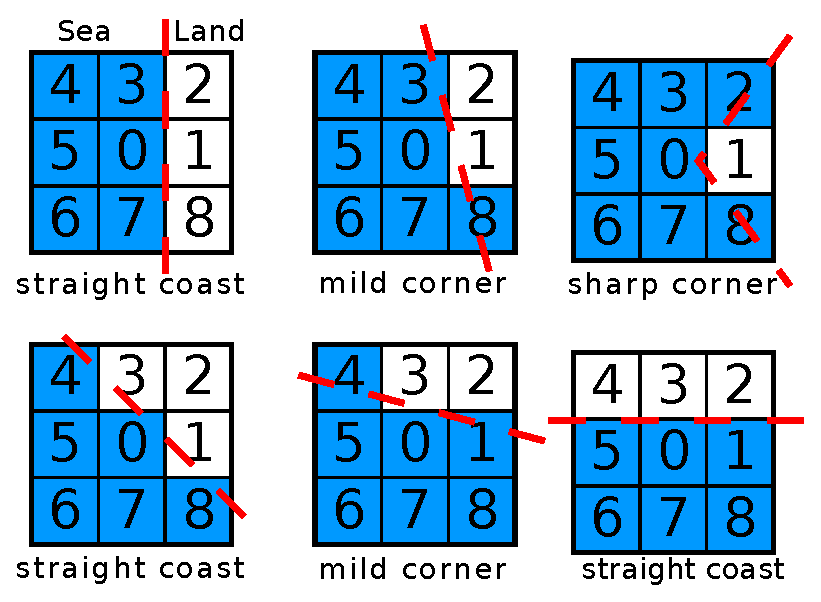
\epsfig{file=./num/coast_reflection.eps,angle=0,width=3in}
\caption{Examples of determination of the shoreline orientation and geometry
  using the land/sea mask. For any sea point (number 0) which is the ocean
  (in blue) and has at least one neighbor in land (in white) the eight
  neighbors, numbered from 1 to 8 are used to define the shoreline geometry.
  For `mild' corners and straight coasts, the estimated shoreline orientation
  (dashed line) is used to compute the directional distribution of the
  reflected wave energy.  }
\label{fig:refl} \botline
\end{center}
\end{figure}

For this purpose we distinguish three different shoreline geometries relative
to the local point as illustrated by Fig. \ref{fig:refl}: we set $n=2$ for a
straight coast (three connected land points among the neighbors), $n=1$ for a
mild corner (two land points among the neighbors), and $n=0$ at a sharp corner
(only one land point, among the 4 closest neighbors) which corresponds to the
same treatment done for sub-grid islands and icebergs. Changing these values
of $n$ in the range $0$ to $2$ has little effect on our results.  $n=1$
corresponds to a Lambertian surface approximation, which is used for
electromagnetic wave scattering from rough surfaces. A pure specular
reflection would be obtained with $n$ infinite.  A more rigorous treatment
should use the distribution of the shoreline orientation at at the scale of
the ocean wavelength, namely of the order of 100~m.

\vsssub
\subsubsection{~Second-order spectrum and free infragravity waves} \label{sec:IG1}
\vsssub

\opthead{IG1}{\ws}{F. Ardhuin}

\noindent 
WARNING: {\it A bug has been identified with IG wave sources in unstructured grids. 
A model patch using an older version of the code will be provided shortly.}

The linear dispersion relation used in section \ref{sec:intro} is a good
approximation for most of the wave energy but a significant part of the
spectrum at high frequencies, with typical frequencies above three times the
windsea wave peak \citep[e.g.][]{rep:Lec13}.  In shallow water, another
strongly nonlinear part of the spectrum is found at very low frequencies,
which are called infragravity waves.

In the case of horizontally homogeneous conditions over a flat bottom, both
low and high frequency non-linear components can be estimated from the linear
wave spectrum, using perturbation theory \citep[e.g.][]{art:Has62}. Also, the
non-linear evolution of a homogeneous wave field is better described in terms
of this `linearized spectrum'. It is thus practical to work with this
`linearized spectrum' and convert to the observable spectrum that contains
non-linear components when post-processing the model results. One method to
perform this transformation is a canonical transformation proposed by
\cite{art:Kra94}. The properties of this transformation were further explored
by \cite{art:Jan09} and implemented for post-processing in the ECMWF version
of the WAM model.

The code for the canonical transform written by P. Janssen was interfaced with
\ws.  Using the {\code IG1} switch and setting the parameter {\code IGADDOUTP
= 2} in the {\F SIG1} namelist, this canonical transformed, which conserves
energy, will be used for the output point spectra.  If {\code IGADDOUTP = 1},
then the second-order spectrum is added on top of the model spectrum using the
theory \citep[e.g.][]{art:Has62}. That option does not conserve energy and
is not consistent at high frequency because the quasi-linear term in the
second-order spectrum are ignored \citep{art:Jan09}.

However, when comparing to measurements, one should be aware that different
measuring devices have different responses to the nonlinear part of the
spectrum. In particular, surface-following buoys also linearize the spectrum,
and the second-order pressure field is not related to the second-order
elevation via the relations used for linear waves. The canonical transform is
thus only applicable for wave gauges that measure elevation at a fixed
location.

When the wave field is not homogeneous, the nonlinear properties of the waves
lead to an exchange of energy between different modes. In shallow water this
usually results in the transfer of energy to infragravity waves, that are
released along shorelines and travel as free waves. The {\code IG1} switch
allows the parameterization of that effect with several methods.  These are
very crude parameterizations compared to the full hydrodynamic solution that
would require solving the bispectral evolution across the surf zone at a very
high spatial resolution \citep[e.g.][]{art:HB97}. The default namelist settings
correspond to the parameterization presented by \cite{art:Aea14}, with minor adjustments in version 6.06. 
The power in the definition of $\widehat{E}_{IG}(f)$ was changed from $f^{1.5}$ to $f^{1.0}$, with 
an associated adjuspent of the constant fro 0.015 to 0.013. 

 In practice the free infragravity wave energy is
added via the $S_{ref}$ source term, by setting the {\code SIG1} namelist
{\code IGSOURCE} to 1 or 2.

In the first method, activated with {\code IGSOURCE =1}, the second-order
spectrum is computed using either the Hasselmann perturbation ({\code IGMETHOD
= 1}) or the canonical transform (any other value of {\code IGMETHOD}) as described 
in \cite{art:Jan09}. This
approach may lead to better directional distribution of IG wave energy but it
is still being tested.  The second method, activated with {\code IGSOURCE =
2}, and the free IG spectrum is given by the following expressions,

\begin{eqnarray}
 A_{IG} & =&    H_s T_{m0,-2}^2\label{eq:IGfit0}, \\
\widehat{E}_{IG}(f)& = & 1.2 \alpha_1^2 \frac{k g^2}{c_g 2 \pi f} \frac{(A_{IG}/4)^2}{\Delta_f}  
\left[\min( 1., 0.013\mathrm{Hz}/ f)\right]^{1.0}, \label{eq:IGfit1} \\
 \widehat{E}_{IG}(f,\theta) & = & \widehat{E}_{IG}(f) / (2 \pi ),
\label{eq:fit2} 
\end{eqnarray}

\noindent
where the mean period is defined as $ T_{m0,-2} =\sqrt{m_{-2}/m_{0}}$ with the
moments

\begin{equation}
 m_n= \int_{f_{min}~\mathrm{Hz}}^{0.5~\mathrm{Hz}} E(f) f^n {\mathrm d}f,\label{eq:mn}
\end{equation}

\noindent
and the empirical coefficient $\alpha_1$ is of the order of
$10^{-3}$~s$^{-1}$, and is set by the {\code SIG1} namelist parameter {\code
IGEMPIRICAL}. The minimum frequency $f_{min}$ used to define $ T_{m0,-2}$ is
set by the namelist parameter {\code IGMAXFREQ} and it is also the maximum
frequency of the IG band over which this source of energy is applied.  Also,
in this band the IG energy at the coast can be added on top of pre-existing
energy, or the pre-existing energy can be reset to zero. That latter behavior
is the default and controlled by {\code IGBCOVERWRITE = 1}. For other choices,
({\code IGBCOVERWRITE = 0}), the results are very sensitive to the maximum
shoreline reflection coefficient allowed ({\code REFRMAX} parameter in
namelist {\F REF1}).

Finally, IG energy can also be added for frequencies beyond $f_{min}$, this is the default behavior 
and it is activated by setting {\code IGSWELLMAX = TRUE}.  For that part of the IG wave
field, the IG wave source is now reduced by a factor 4 which is now hard-coded
in {\file w3ref1md.ftn}. This should be adjusted together with the maximum reflection 
which is defined by the {\F REF1} namelist parameter {\code
REFRMAX}. In the present version, the option {\code IGSWELLMAX = TRUE} does 
not work well with unstructured grids. We thus advise to use 
{\code IGSWELLMAX = FALSE} for these grids, this will unfortunately lead 
to a spectral gap between the IG band and the swell-windsea band. 





\vspace{\baselineskip}
\vssub
\subsection{~Air-sea processes}
\vsssub
\subsubsection{~General concepts}
\vsssub

Additional subroutines are provided within \ws\ for use as part of coupled ocean-wave or ocean-atmosphere systems.
These subroutines are designed to compute additional quantities related to the surface wave field which are intended to be passed to external models (e.g. ocean models).
The motivation for these subroutines is to allow the external model to include the impact of waves on quantities such as the wind stress and the upper ocean turbulence.

\paragraph{Sea-state dependent air-sea fluxes}

The air-sea momentum flux, or the total wind stress, is the sum of the momentum flux into both surface waves and subsurface currents.
Coupled atmosphere-ocean models that do not consider the impact of the surface gravity wave field typically compute the total wind stress based on an empirical relationship between the wind speed and the wind stress (via a drag coefficient, $C_d$).
The provided {\it FLD} subroutines allows the computation of the total wind stress based on the \ws\ wavenumber-direction spectrum for use in coupled numerical models.

To the leading order, the total wind stress is equal to the sum of the momentum flux into surface waves (form drag of surface waves) and the momentum flux directly into the subsurface currents (through viscous stress).
The momentum flux into the waves may be expressed as an integral of the wave variance spectrum multiplied by the wave growth rate (momentum-uptake rate).
A few assumptions are needed to calculate the wave form drag.
First, the wave form drag is sensitive at the leading order to the level of the high frequency waves (or the spectral tail).
This part of the wave spectrum contains a great deal of uncertainty within the wave model, and therefore may need to be separately parameterized for computing the wind stress.
An assumption must therefore be made to parameterize the high frequency, which is not constrained by observational data and wind speeds above 15 m/s.
Second, assumptions of the wave growth-rate function are needed since it has historically been parameterized from either the wind speed or the wind stress.
In either case, empirical coefficients are needed within the growth-rate function based on wavelength and wave direction relative to the wind and/or stress.
Third, there is feedback due to the wave form drag on the turbulence profile and the wind profile within the wave boundary layer (roughly the upper 10 meters above the air-sea interface).
How important this feedback is on determining the wind stress and the mean wind profile is not entirely understood.
Finally, the growth rate is known to be different over breaking and non-breaking waves.
However, there are no simple methods for explicitly including the breaking wave impact within wind-stress calculation models.
Therefore, no separation is made in either of the present {\it FLD} subroutines between breaking and non-breaking wave growth-rates.

The total air-sea momentum flux can be expressed (to the leading order) as:
\begin{equation}
\vec{\tau}=\vec{\tau}_{\nu}+\vec{\tau}_{f},
\end{equation}
where $\vec{\tau}_{\nu}$ is the viscous stress vector and $\vec{\tau}_{f}$ is the wave form drag.
At the air-sea interface, the wave form drag can be computed as the contribution of the momentum flux into all waves:
\begin{equation}\label{formdrag}
\vec{\tau}_{f}=\rho_w\int_{k_{min}}^{k_{max}}\int_{-\pi}^{\pi} \beta_g(k,\theta) \sigma F (k,\theta) d\theta \vec{k} dk,
\end{equation}
where $\rho_w$ is the water density, $k$ is the wavenumber, $\theta$ is the wave direction, $\sigma$ is the angular frequency, $\beta_g (k,\theta)$ is the growth rate,
$F (k,\theta)$ is the wave variance spectrum, and $k_{min}$ and $k_{max}$ are the minimum and maximum wavenumbers of contributing waves.
The expression for the growth rate varies based on the theory applied in the model, and will be described separately for each theory in their following descriptions.

The spectral tail at wind speeds above 15 m/s is not well constrained observationally or theoretically.
Therefore, the spectral tail level in the {\it FLD} subroutines has been empirically parameterized such that the mean drag coefficient corresponds to the standard bulk drag coefficient used within the modeling system.
In this way, the mean value of the wind stress will not be modified by using any explicit sea state dependent wind stress formulation, but the stress will deviate from the mean based on the sea-state.
It is assumed that the tail level is a function of a wind speed only and is independent of sea states.
\vsssub
\subsubsection{~Sea-state dependent $\tau$: Reichl et al. 2014} \label{sec:FLD1}
\vsssub

\opthead{FLD1}{\ws}{B. Reichl}

\paragraph{Wind stress according to Reichl et al., 2014}

In \citet{art:Rei14} the total stress is constant in height, but is decomposed into two components as a function of height as:
\begin{equation}
\vec{\tau}=\vec{\tau}_t(z)+\vec{\tau}_f(z),
\end{equation}
where $\tau_t$ is the turbulent stress and is equal to the viscous stress very near the surface.
The wave form stress can be expressed as:
\begin{equation}
\vec{\tau}_f(z)=\rho_w\int^{k=\delta/z}_{k_{min}} \int^\pi_{-\pi}\beta_g(k,\theta) \sigma F(k,\theta) d\theta {\vec{k}} dk,
\end{equation}
that is, the wave form stress at height $z$ is equal to the integration of the wave form stress at the surface for wavenumbers below $k=\delta/z$, where $\delta/k$ is the inner layer height \citep{art:Har04} for waves at a wavenumber $k$.
This expression is derived by assuming that the wave-induced stress is significant from the surface up to the inner layer height, but is negligible further above.
Since at the surface
\begin{equation}
\vec{\tau}=\vec{\tau}_\nu+\vec{\tau}_f(z=0)=\vec{\tau}_\nu+\rho_w\int^{k_{max}}_{k_{min}} \int^\pi_{-\pi}\beta_g(k,\theta) \sigma F(k,\theta) d\theta {\vec{k}} dk,
\end{equation}
the turbulent stress at a height $z$ can be expressed as:
\begin{equation}
\vec{\tau}_t(z)=\vec{\tau}_\nu+\rho_w\int^{k_{max}}_{k=\delta/z} \int^\pi_{-\pi}\beta_g(k,\theta) \sigma F(k,\theta) d\theta {\vec{k}} dk.
\end{equation}

In this model it is assumed that the turbulent stress at the inner layer height $z=\delta/k$ determines the growth rate of waves at wavenumber $k$:
\begin{equation}
\beta_g(k,\theta)=c_\beta \sigma\frac{\left|\tau_t(z=\delta/k)\right|}{\rho_wc^2}\cos^2(\theta-\theta_\tau),
\end{equation}
where $\theta_\tau$ is the direction of the turbulent stress at the inner layer height.
The turbulent stress at the inner layer height is used in place of the total wind stress because longer waves reduce the effective wind forcing on shorter waves (wave sheltering).

The growth rate coefficient $c_\beta$ varies depending on the ratio of the wave phase speed to the local turbulent friction velocity (friction velocity at the inner layer height), $u_\star^l=\sqrt{\tau_t(z=\delta/k)/\rho_a)}$.
\begin{equation}
c_{\beta}=\left\{
\begin{array}{cll} 
25  &: \cos(\theta-\theta_w)>0 \hspace{2mm}&:c/u_{\star}^l<10\\
10+15\cos[\pi(c/u_\star-10)/15]   &:&:10\le c/u_{\star}^l<25 \\
-5  &:&:25\le c/u_{\star}^l\\
-25  &: \cos(\theta-\theta_w)<0 &\\
\end{array}
\right.
\end{equation}

The wind profile is explicitly calculated using the energy conservation constraint in the wave boundary layer.
From the top of the viscous sublayer to the inner layer height of the shortest waves the wind shear is expressed as:
\begin{equation}
\frac{d {\vec{u}}}{\partial z}=\frac{\rho_a}{\kappa z}\left|\frac{ \vec{\tau}_\nu}{\rho_a}\right|^{3/2}\frac{\vec{\tau}_\nu}{\vec{\tau}_\nu\cdot\vec{\tau}_{tot}}\hspace{3mm}{\rm for}\hspace{3mm}z_\nu<z<\delta/k_l.
\end{equation}
Between the inner layer height of the shortest waves and that of the longest waves the wind shear is expressed as:
\begin{equation}
\frac{d {\vec{u}}}{\partial z}=\left[ \frac{\delta}{z^2}\tilde{F}_w\left(k=\frac{\delta}{z}\right)+\frac{\rho_a}{\kappa z}\left| \frac{\vec{\tau}_t(z)}{\rho_a}\right|^{3/2} \right]\times\frac{\vec{\tau}_t(z)}{\vec{\tau}_t(z)\cdot\vec{\tau}_{tot}}\hspace{3mm}{\rm for}\hspace{3mm}\delta/k_l\le z,
\end{equation}
where $\tilde{F}_w(k=\delta/z)$ is the energy uptake by surface waves:
\begin{equation}
\tilde{F}_w(k=\delta/z)=\rho_w\int^{\pi}_{-\pi}\beta_g(k,\theta)gF(k,\theta)k d\theta.
\end{equation}
Finally, above the inner layer height of the longest waves the wave effect is negligible and the wind shear is aligned in the direction of the wind stress:
\begin{equation}
\frac{d{\vec{u}}}{dz}=\frac{u_\star}{\kappa z}\frac{\vec{\tau}_{tot}}{|\vec{\tau}_{tot}|}.
\end{equation}

Note that when using the FLD1 switch, internal variables and output values of the viscous stress, friction velocity, surface roughness length and Charnock parameter are recalculated and overwritten. 

\vsssub
\subsubsection{~Sea-state dependent $\tau$: Donelan et al. 2012} \label{sec:FLD2}
\vsssub

\opthead{FLD2}{UMWM}{B. Reichl}

\paragraph{Wind stress according to Donelan et al., 2012}
In \citet{art:Don12} the growth rate parameter in Eq. (\ref{formdrag}) is expressed as:
\begin{equation}
\beta_g(k,\theta)=A_1 \sigma \frac{\left[u_{\lambda/2} \cos(\theta-\theta_w)-c\right]\left| u_{\lambda/2}cos(\theta-\theta_w)-c \right|}{c^2}\frac{\rho_a}{\rho_w},
\end{equation}
\begin{equation}
A_{1}=\left\{
\begin{array}{lll} 
0.11, & :  u_{\lambda/2}\cos\theta>c,  &\mbox{for wind forced sea}\\
0.01 & :   0<u_{\lambda/2}\cos\theta<c, &\mbox{for swell faster than the wind}\\
0.1 & :  \cos\theta<0,  &\mbox{for swell opposing the wind}
\end{array}
\right.
\end{equation}
where $A_1$ is the proportionality coefficient determined empirically (so that modeled wave spectra agree with field observations), $u_{\lambda/2}$ is the wind speed at the height of half the wavelength (up to 20 m), $\theta_w$ is the wind direction, and $c$ is the wave phase speed.
The wind speed is calculated using the law of the wall for rough surfaces:
\begin{equation}
u(z)=\frac{u_\star}{\kappa}\ln\left(\frac{z}{z_0}\right),
\end{equation}
where $\kappa$ is the von K\'arm\'an coefficient (default 0.4).
The viscous stress is calculated from the law of the wall for smooth surfaces.
The viscous drag coefficient, $Cd_\nu$ is adjusted to account for sheltering:
\begin{equation}
Cd'_\nu=\frac{Cd_\nu}{3}\left(1+\frac{2 Cd_\nu}{Cd_\nu+Cd_f}\right),
\end{equation}
where $Cd_f$ is the wave form drag coefficient.
The viscous stress can then be solved for as:
\begin{equation}
\vec{\tau}_\nu=\rho_a Cd'_\nu \left|{\bf u_{z}}\right|{\bf {u}}_{z}.
\end{equation}

Note that when using the FLD2 switch, internal variables and output values of the viscous stress, friction velocity, surface roughness length and Charnock parameter are recalculated and overwritten. 

\vspace{\baselineskip}
\vssub
\subsection{~Output parameters} \label{sub:outpars}
\vssub

The wave model can output parameters on the geographical grid of the model that can be integrated parameters or 
parameters as a function of frequency, with one grid for each frequency. All parameters that are a function of frequency (e.g.  \textbf{EF} or \textbf{USF}) require the setting 
of specific namelist parameters in the {\F OUTS} namelist defined in ww3\_grid.inp or  ww3\_grid.nml . This is to reduce the memory use
if these parameters are not needed. 

Below, a brief definition of output field parameters is provided. A table
with definitions may be found in the sample {\code ww3\_shel.inp} file,
in \para\ref{sec:ww3shel}. That input file also provides a list of flags  
indicating if output parameters are available in different field
output file types (ASCII, grib, igrads, NetCDF). 
For any details on how these parameters are computed, the user may read the code of the  {\code w3iogo} routine, in the {\code w3iogomd.ftn} module. 

Selection of field outputs in  {\code ww3\_shel.inp} is most easily performed by providing a list of the 
requested parameters, for example, {\textbf HS DIR SPR}  will request the calculation of significant wave height, mean direction and directional spread. These will thus be stored in the {\code out\_grd.XX} file and can be post-processed, for example in NetCDF using   {\code ww3\_ouf}. Examples are given in \para\ref{sec:ww3multi} and
\para\ref{sec:ww3ounf}. The names for these namelists are the bold names below, for 
example \textbf{HS}. 

All parameters listed below are available in ASCII and NetCDF output files. If selected output file types are grads or grib, some parameters may not be available. Availability (or not) is identified
in the first two columns in the field output parameter table within the example input file in  
\para\ref{sec:ww3shel}. That table also identifies, for all parameters,
the internal WAVEWATCH III code tags, the output tags (names used is ASCII 
file extensions, NetCDF variable names and namelist-based selection (see 
also \para\ref{sec:ww3ounf}), and the long parameter name/definition.

Finally we note that in all definitions the frequency is the \emph{relative} frequency. Thus, in the presence of currents, these can only be compared to drifting measurement data or data obtained in wavenumber and converted to frequency. Comparison to fixed instrument data requires the use of the full spectrum and proper conversion to the fixed reference frame.

\begin{list}{\Roman{outgrps})\hfill}
            {\usecounter{outgrps} \leftmargin 7mm \labelwidth 5mm
             \rightmargin 0mm \itemsep \baselineskip \parsep 0mm}

\item {Forcing fields}

\begin{list}{\arabic{outpars})\hfill}
            {\usecounter{outpars} \leftmargin 8mm \labelwidth 7mm
             \rightmargin 0mm \itemsep 0mm \parsep 0mm}
\item \textbf{DPT} The mean water depth (m). This includes varying water levels. 
\item \textbf{CUR} The mean current velocity (vector, m/s).
\item \textbf{WND} The mean wind speed (vector, m/s). This wind speed is always the
      speed as input to the model, i.e., is not corrected for the current
      speed.
\item \textbf{AST} The air-sea temperature difference ($^\circ$C).
\item \textbf{WLV} Water level.
\item \textbf{ICE} Ice concentration.
\item \textbf{IBG} Wave attenuation due to icebergs: this parameter is the inverse of the
  e-folding scale associated to the loss of wave energy in a field of small
  icebergs \citep{art:Aea11}.
\item \textbf{D50} Sediment median grain size ($D_{50}$). 
\item \textbf{IC1} Ice thickness. 
\item \textbf{IC5} Maximum ice flow diameter, $D_{\max}$. 
\end{list}

\item{Standard mean wave parameters}

\begin{list}{\arabic{outpars})\hfill}
            {\usecounter{outpars} \leftmargin 8mm \labelwidth 7mm
             \rightmargin 0mm \itemsep 0mm \parsep 0mm}
\item \textbf{HS} Significant wave height (m) [see Eq.~(\ref{eq:etot})]
      \begin{equation} H_s = 4 \sqrt{E} \: . \label{eq:Hs} \end{equation}
\item \textbf{LM} Mean wave length (m) [see Eq.~(\ref{eq:zbar})]
      \begin{equation} L_m = 2\pi \overline{k^{-1}}
      \: . \label{eq:Lm} \end{equation}
\item \textbf{T02} Mean wave period (s) [see Eq.~(\ref{eq:zbar})]
      \begin{equation} T_{m02} = 2\pi /\sqrt{\overline{\sigma^{2}}}
      \: . \label{eq:Tm02} \end{equation}
\item \textbf{T0M1} Mean wave period (s) [see Eq.~(\ref{eq:zbar})]
      \begin{equation} T_{m0,-1} = 2\pi \overline{\sigma^{-1}}
      \: . \label{eq:Tm0m1} \end{equation}
\item \textbf{T01} Mean wave period (s) [see Eq.~(\ref{eq:zbar})]
      \begin{equation} T_{m0,1} = 2\pi /\overline{\sigma}
      \: . \label{eq:Tm} \end{equation}
\item \textbf{FP} Peak frequency (Hz), calculated from the one-dimensional frequency
      spectrum using a parabolic fit around the discrete peak.
\item \textbf{DIR} Mean wave direction (degr., meteorological convention)
      \begin{equation} \theta_m = \mbox{atan} \left ( \frac{b}{a} \right )
      \: , \label{eq:theta_m} \end{equation} \begin{equation}
      a = \int_0^{2\pi} \int_0^\infty \cos(\theta) F(\sigma,\theta) \:
      d\sigma \: d\theta \: , \end{equation} \begin{equation}
      b = \int_0^{2\pi} \int_0^\infty \sin(\theta) F(\sigma,\theta) \:
      d\sigma \: d\theta \: . \end{equation}
\item \textbf{SPR} Mean directional spread \citep[degr.;][]{art:KVH88}
      \begin{equation} \sigma_\theta = \left [ 2 \left \{ 1 - \left (
      \frac{a^2+b^2}{E^2} \right )^{1/2} \right \} \right ]^{1/2}
      \: , \label{eq:sig_th} \end{equation}
\item \textbf{DP} Peak direction (degr.), defined like the mean direction, using the
      frequency/wavenumber bin containing of the spectrum $F(k)$ that
      contains the peak frequency only.
\item \textbf{HIG} Infragravity height.
\item \textbf{MXE}   Max surface elev (Space-time extreme, STE)
\item \textbf{MXES}  St Dev of max surface elev (STE)
\item \textbf{MXH}  Max wave height (STE)
\item \textbf{MXHC}  Max wave height from crest (STE)
\item \textbf{SDMH}  St Dev of MXC (STE)
\item \textbf{SDMHC} St Dev of MXHC (STE)
\item \textbf{WBT}   Dominant wave breaking probability $b_T$ (\ref{eq:bt})
\item \textbf{TP} Peak wave period, derived from reciprocal of peak freq
(\textbf{FP}).
\end{list}

\item{Spectral parameters (first 5 moments and wavenumbers). 

All these parameters are a function 
of frequency and thus these are three-dimensional arrays. Because of the large memory use, the 
computation of these parameters requires the activation of switches in the {\F OUTS} namelist.}

\begin{list}{\arabic{outpars})\hfill}
            {\usecounter{outpars} \leftmargin 8mm \labelwidth 7mm
             \rightmargin 0mm \itemsep 0mm \parsep 0mm}
   
\item \textbf{EF} Wave frequency spectrum (m$^2$/Hz)
      \begin{equation} E(f) = 2 \pi  \int F(\sigma,\theta) \mathrm{d} \theta 
      \: . \label{eq:Ef} \end{equation}
\item \textbf{TH1M} Mean direction for each frequency  \citep[degr.;][]{art:KVH88}
       \begin{equation} \theta_1 (f)= \mbox{atan} \left ( \frac{b_1(f)}{a_1(f)} \right )
      \: , \label{eq:theta_b} \end{equation} \begin{equation}
      a_1(f) = 2 \pi \int_0^{2\pi} \int_0^\infty \cos(\theta) F(\sigma,\theta) \:
       \mathrm{d}\theta \: , \end{equation} \begin{equation}
      b_1(f) = 2 \pi \int_0^{2\pi} \int_0^\infty \sin(\theta) F(\sigma,\theta) \:
       \mathrm{d}\theta \: . \end{equation}
\item \textbf{STH1M} First directional spread for each frequency  (degr.; )
      \begin{equation} \sigma_1(f) = \left [ 2 \left \{ 1 - \left (
      \frac{a_1(f)^2+b_1(f)^2}{E(f)^2} \right )^{1/2} \right \} \right ]^{1/2}
      \: , \label{eq:sig_th1} \end{equation}
\item \textbf{TH2M} Mean direction from $a_2$ and $b_2$ (degr.)
       \begin{equation} \theta_2 (f)= \mbox{atan} \left ( \frac{b_2(f)}{a_2(f)} \right )
      \: , \label{eq:theta_2} \end{equation} \begin{equation}
      a_2(f) = 2 \pi \int_0^{2\pi} \int_0^\infty \cos(2 \theta) F(\sigma,\theta) \:
       \mathrm{d}\theta \: , \end{equation} \begin{equation}
      b_2(f) = 2 \pi \int_0^{2\pi} \int_0^\infty \sin(2 \theta) F(\sigma,\theta) \:
       \mathrm{d}\theta \: . \end{equation}
\item \textbf{STH2M} Directional spreading from $a_2$ and $b_2$ (degr.)  
      \begin{equation} \sigma_2(f) = \left [ 0.5 \left \{ 1 - \left (
      \frac{a_2(f)^2+b_2(f)^2}{E(f)^2} \right )^{1/2} \right \} \right ]^{1/2}
      \: , \label{eq:sig_th1} \end{equation}
\item \textbf{WN}  Wavenumbers $k(\sigma)$ (rad/m)
      \begin{equation} \sigma^2 = g k \tanh (k D) 
      \: , \label{eq:k} \end{equation}
\end{list}

\item{Spectral partition parameters} \label{out:spec_part}

These output parameters are based on
partitioning of the spectrum into individual wave fields.

\begin{list}{\arabic{outpars})\hfill}
            {\usecounter{outpars} \leftmargin 8mm \labelwidth 7mm
             \rightmargin 5mm \itemsep 0mm \parsep 0mm}


\item \textbf{PHS}  Wave heights $H_s$ of partitions of the spectrum (see
      below). \label{out:first_part}
\item \textbf{PTP} Peak (relative) periods of partitions of the spectrum (parabolic fit).
\item \textbf{PLP} Peak wave lengths of partitions of the spectrum (from peak period).
\item \textbf{PSP} Mean direction of partitions of the spectrum.
\item Directional spread of partition of the spectrum
      Cf. Eq.~(\ref{eq:sig_th}).
\item \textbf{PWS} Wind sea fraction of partition of the spectrum.  The method of
\cite{art:HP01} is used, implemented as described in \cite{tol:Oahu07a}. With
this, a `wind sea fraction' $W$ is introduced
\begin{equation}
W = E^{-1}  \: E |_{U_p > c}  \:\:\: , \label{eq:wsf}
\end{equation}
where $E$ is the total spectral energy, and $E |_{U_p > c}$ is the energy in
the spectrum for which the projected wind speed $U_p$ is larger than the local
wave phase velocity $c = \sigma / k$. The latter defines an area in the
spectrum under the direct influence of the wind. To allow for nonlinear
interactions to shift this boundary to lower frequencies, and subsequently to
have fully grown wind seas inside this are, $U_p$ includes a multiplier
$C_{mult}$
\begin{equation}
U_p = C_{mult} U_{10} \cos ( \theta - \theta_w )  \:\:\: . \label{eq:Up}
\end{equation}
The multiplier can be set by the user. The default value is $C_{mult} = 1.7$.
\item \textbf{PDP} Peak direction of partitions of the spectrum.
\item \textbf{PQP} Goda peakedness of partitions of the spectrum.
\item \textbf{PPE} JONSWAP peak enhancement factor of partitions
      of the spectrum. It is a measure of amplification
      of the spectral peak to the peak of the corresponding
      \citeauthor{art:PM64} spectrum.
\item \textbf{PGW} Gaussian frequency width (Hz) of partitions of the spectrum.
      Least-square fit of a Gaussian spectrum to the one-dimensional spectral partition.
\item \textbf{PSW} Spectral width of partitions of the spectrum \citep{art:LH84}
\item \textbf{PTE} Wave energy period of partitions of the spectrum [see Eq.~(\ref{eq:Tm0m1})] 
\item \textbf{PT1} Mean wave period of partitions of the spectrum [see Eq.~(\ref{eq:Tm})] 
\item \textbf{PT2} Wave zero-upcrossing period of partitions of the spectrum [see Eq.~(\ref{eq:Tm02})]
\item \textbf{PEP} Wave peak spectral density of partitions
\item \textbf{TWS} Wind sea fraction of the entire spectrum.
\item \textbf{PNR} Number of partitions found in the spectrum. \label{out:last_part}
\end{list}


\item{Atmosphere-waves layer}
\begin{list}{\arabic{outpars})\hfill}
            {\usecounter{outpars} \leftmargin 8mm \labelwidth 7mm
             \rightmargin 0mm \itemsep 0mm \parsep 0mm}
\item \textbf{UST}  The friction velocity $u_\ast$ (scalar). Definition depends on
      selected source term parameterization (m/s). An alternative vector version
      of the stresses is available for research (requires user intervention in
      the code).
\item \textbf{CHA}  Charnock parameter for air-sea friction (without dimensions)
\item \textbf{CGE} Energy flux (W/m)
      \begin{equation} C_g E =  \rho_w g \overline{C_g} E
      \: . \label{eq:CgE} \end{equation}
\item \textbf{FAW} Wind to wave energy flux
\item \textbf{TAW} Net wave-supported stress (wind to wave momentum flux) 
\item \textbf{TWA} Negative part of the wave-supported stress
\item \textbf{WCC} Whitecap coverage (without dimensions)
\item \textbf{WCF} Wave to wind momentum flux 
\item \textbf{WCH} Whitecap mean thickness (m) 
\item \textbf{WCM} Mean breaking wave height (m) (NOT AVAILABLE YET)
%\item \textbf{PWS} Moment of whitecap distribution (?) (NOT PLUGGED YET)
\end{list}

\item{Wave-ocean layer}

\begin{list}{\arabic{outpars})\hfill}
            {\usecounter{outpars} \leftmargin 8mm \labelwidth 7mm
             \rightmargin 0mm \itemsep 0mm \parsep 0mm}
\item \textbf{SXY} Radiation stresses
      \begin{equation} S_{xx} = \rho_w g \int \!\!\!\! \int \left
        ( n - 0.5 + n \cos^2 \theta \right )  \: F(k,\theta) \: dk d\theta
      \: , \label{eq:Sxx} \end{equation}
      \begin{equation} S_{xy} =\rho_w g \int \!\!\!\! \int
        n \sin \theta \cos \theta  \: F(k,\theta) \: dk d\theta
      \: , \label{eq:Syy} \end{equation}
      \begin{equation} S_{yy} =\rho_w g \int \!\!\!\! \int \left
        ( n - 0.5 + n \sin^2 \theta \right )  \: F(k,\theta) \: dk d\theta
      \: , \label{eq:Sxy} \end{equation}
      where
      \begin{equation} n = \frac{1}{2} + \frac{kd}{\sinh 2kd}
      \: . \label{eq:n} \end{equation}
\item \textbf{TWO} Wave to ocean momentum flux (m$^2$/s$^2$)
\item \textbf{BHD} Bernoulli head (m$^2$/s$^2$)
      \begin{equation} J =  g \int \!\!\!\! \int  \frac{k}
        {\sinh 2kd}  \: F(k,\theta) \: dk d\theta
      \: , \label{eq:BHD} \end{equation}
\item \textbf{FOC} Wave to ocean energy flux (W/m$^2$)
\item \textbf{TUS} Stokes volume transport (m$^2$/s)
     \begin{equation} (M^w_x,M^w_y) =  g \int \!\!\!\! \int  \frac{(k \cos(\theta),k \sin(\theta))}
        {\sigma}  \: F(k,\theta) \: dk d\theta
      \: , \label{eq:Mw} \end{equation}
\item \textbf{USS} Stokes drift at the sea surface (m/s)
     \begin{equation} (U_{ssx},U_{ssy}) =  \int \!\!\!\! \int  \sigma \cosh 2kd \frac{(k \cos(\theta),k \sin(\theta))}
        {\sinh^2 kd}  \: F(k,\theta) \: dk d\theta
      \: , \label{eq:Uss} \end{equation}
\item \textbf{P2S} Second order pressure variance (m$^2$) and peak period of this pressure (s) which contributes to acoustic and seismic noise, 
      \begin{equation} F_{p2D}(k=0) = \int_0^{\infty} \frac{4 \sigma}{C_g} \int_0^{\pi}  F(k,\theta) \:  F(k,\theta+\pi) \:  d\theta dk
      \: , \label{eq:sop} \end{equation}
\item \textbf{USF} Frequency spectrum of Stokes drift at the sea surface (m/s/Hz)
     \begin{equation} (U_{ssx}(f),U_{ssy}(f)) =  \int \sigma \cosh 2kd \frac{(k \cos(\theta),k \sin(\theta))}
        {\sinh^2 kd}  \: F(k,\theta) \frac{2 \pi}{C_g} d\theta
      \: , \label{eq:Ussf} \end{equation}
Note that US3D=1 must be set in the ww3\_grid.inp OUTS namelist in order to activate the 3D arrays needed for USF output.
\item \textbf{P2L} Frequency spectrum of the second order pressure (m$^2$s)  which contributes to acoustic and seismic noise,
      \begin{equation} F_{p2D}(k=0,f) =  \frac{2 \sigma}{\pi} \int_0^{\pi}  \frac{4 \pi^2}{C_g^2} F(k,\theta) \:  F(k,\theta+\pi) \:  d\theta
      \: . \label{eq:sopf} \end{equation}
\item \textbf{TWI}   Wave to sea ice stress
\item \textbf{FIC}   Wave to sea ice energy flux
\item \textbf{USP}   Surface Stokes drift partitioned into run-time defined frequency components (m/s),
      \begin{equation} (U_{ssp},V_{ssp})(n) =  \int \!\!\!\! \int_{k_n}  \sigma \cosh 2kd \frac{(k\
      \cos(\theta),k \sin(\theta))}
        {\sinh^2 kd}  \: F(k,\theta) \: dk d\theta
      \: . \label{eq:Ussp} \end{equation}
The number $n$ and the central wavenumbers for the partitions $k_n$ are `run-time' in the sense that they are defined in the model definition file generated from ww3\_grid.inp (see the sample input file for details on setting these quantities).  The wavenumber integral bounds for each $n$ partition divide the model wave spectra to accomodate the prescribed values of $k_n$.
\item \textbf{TOC} Total ocean stress (Pa)
      \begin{equation} \tau_{oc} = \tau_a - \tau_{aw} + \tau_{woc}
      \: . \label{eq:Toc} \end{equation}
\end{list}

\item{Wave-bottom layer}

\begin{list}{\arabic{outpars})\hfill}
            {\usecounter{outpars} \leftmargin 8mm \labelwidth 7mm
             \rightmargin 0mm \itemsep 0mm \parsep 0mm}

\item \textbf{ABR} Near-bottom rms excursion amplitude
      \begin{equation} a_{b,rms} = \left [ 2 \int \!\!\!\! \int
      \frac{1}{\sinh^2 kd} \: F(k,\theta) \: dk d\theta \right ] ^{1/2}
      \: . \label{eq:ab_rms} \end{equation}
\item \textbf{UBR} Near-bottom rms orbital velocity
      \begin{equation} u_{b,rms} = \left [ 2 \int \!\!\!\! \int
      \frac{\sigma^2}{\sinh^2 kd} \: F(k,\theta) \: dk d\theta \right ] ^{1/2}
      \: . \label{eq:ub_rms} \end{equation}
\item \textbf{BED} Bedform parameters: ripple height and directions (NOT TESTED YET)   
\item \textbf{FBB} Energy dissipation in WBBL 
\item \textbf{TBB} Momentum loss in WBBL 
\end{list}

\item{Spectrum parameters}

\begin{list}{\arabic{outpars})\hfill}
            {\usecounter{outpars} \leftmargin 8mm \labelwidth 7mm
             \rightmargin 0mm \itemsep 0mm \parsep 0mm}

\item \textbf{MSS} Mean square slopes in $u$ and $c$ directions (down-wave and cross-wave components of slopes variances). 
\item \textbf{MSC} Spectral tail level (without dimensions) 
\item \textbf{MSD} Direction of the maximum slope variance mss$_u$
\item \textbf{MCD} Spectral tail direction
\item \textbf{QP}  Peakedness parameter \citep{art:G70}
      \begin{equation} Q_p = \frac{2}{E^2} \int_0^{2\pi} \int_0^\infty
      \sigma\:F(\sigma,\theta)^2\:d\sigma\:d\theta \: \label{eq:qp}
      \end{equation}
\end{list}

\item{Numerical diagnostics }

\begin{list}{\arabic{outpars})\hfill}
            {\usecounter{outpars} \leftmargin 8mm \labelwidth 7mm
             \rightmargin 0mm \itemsep 0mm \parsep 0mm}
\item \textbf{DTD} Average time step in the source term integration (s).
\item \textbf{FC} Cut-off frequency $f_c$ (Hz, depends on parameterization of
      input and dissipation).
\item \textbf{CFX} Maximum CFL number for spatial advection 
\item \textbf{CFD} Maximum CFL number for angular advection 
\item \textbf{CFK} Maximum CFL number for wavenumber advection 
\end{list}

\item{User defined }

\begin{list}{\arabic{outpars})\hfill}
            {\usecounter{outpars} \leftmargin 8mm \labelwidth 7mm
             \rightmargin 0mm \itemsep 0mm \parsep 0mm}

\item \textbf{U1} Slot for user defined parameter (requires modification of code).
\item \textbf{U2} Idem.
\end{list}

\end{list}




%\vspace{\baselineskip}
%\centerline{\ldots NEEDS CLEAN UP BELOW HERE \ldots}
%\vspace{\baselineskip}

%THESE TWO PARAMETERS WILL BE PUT BACK. 
%Old output types \ref{out:old_fpw} and \ref{out:old_thw} have become obsolete
%with the introduction of the partitioned output types \ref{out:first_part}
%through \ref{out:last_part}. However, they are retained in the present model
%release to provide required downward compatibility with model version 1.18 at
%NCEP. These output types are likely to be retired in upcoming versions of \ws.

\vssub
\subsection{~Derived parameters} \label{sub:outpars}
\vssub

\subsubsection{Directional slopes and near-nadir backscatter}
Under the linear wave assumption, the surface slopes are Gaussian and fully prescribed by the 
mean square slope tensor mss$_x$, mss$_y$, mss$_{xy}$. In \ws\ the computed mss parameters are the down-wave $\mathrm{mss}_u$, which is 
in the direction given by $\mathrm{mss}_d$, and a cross-wave $\mathrm{mss}_c$ which is in the perpendicular dimension. 

As a a result, the 
mean square slope tensor for the (long) wave resolved by the wave model, after converting $\mathrm{mss}_d$ to radians, are given by 
\begin{eqnarray}
   \mathrm{mss}_{x,\mathrm{long}} &=& \mathrm{mss}_u \cos^2(\mathrm{mss}_d)+\mathrm{mss}_c \sin^2(\mathrm{mss}_d) \\
   \mathrm{mss}_{y,\mathrm{long}} &=& \mathrm{mss}_u \sin^2(\mathrm{mss}_d)+\mathrm{mss}_c \cos^2(\mathrm{mss}_d) \\
   \mathrm{mss}_{xy,\mathrm{long}}&=&0.5 (\mathrm{mss}_u - \mathrm{mss}_c) \sin(2 \mathrm{mss}_d)
\end{eqnarray}
The contribution of short waves (above the maximum frequency of the model) should be added to these for a comparison with observations 
such as the backscatter power ($\sigma^0$) of near-nadir optical or radar data (altimeters, GPM or CFOSAT/SWIM data).
   
\subsubsection{Stokes drift profile}
The spectrum of the surface Stokes drift has the two components that are computed as \\
{\code usf(IK)= SUM( E(IK,ITH)*ECOS(ITH)*DTH(ITH) )*DK(IK)*2*WN(IK,ISEA) *  FACT(KD)/DF(IK)}

{\code vsf(IK)= SUM( E(IK,ITH)*ESIN(ITH)*DTH(ITH) )*DK(IK)*2*WN(IK,ISEA) *  FACT(KD)/DF(IK)}

Where WN is the wavenumber and FACT(KD) is a function of the non-dimensional water depth.

From this spectrum, the Stokes drift at any depth $z$, counted positive upwards from a reference $z=0$, are given by

Us(z)= SUM{IK=I1,I2} ( usf(IK) * FACT2(z,KD)*DF(IK))
Vs(z)= SUM{IK=I1,I2} ( vsf(IK) * FACT2(z,KD)*DF(IK))

This requires a knowledge of the local water depth D and mean sea level LEV and the wavenumbers WN(IK). KD=D*WN(IK) is thus a local function if the frequency/wavenumber index IK.

The coefficent FACT2(z,KD) is equal to EXP(2*WN(IK)*(z-LEV)) if KD $>$ 6, and otherwise, \\
FACT2(z,KD)=COSH(2*WN(IK)*(z+H))/COSH(2*WN(IK)*D).


\bpage
